% This file (dissertation-main.tex) is the main file for a dissertation.
\documentclass {udthesis}

\usepackage{multirow}
\usepackage{amsmath}
\usepackage{amsfonts}
\usepackage{amsthm}
\usepackage{amssymb}
\usepackage{algorithm}[0.1]
\usepackage{algorithmic}[0.1]
\usepackage{subfig}
\usepackage{graphics}

\newtheorem{thm}{Theorem}[section]

\DeclareGraphicsExtensions{.eps}

\newcommand{\lp}{\left(}
\newcommand{\rp}{\right)}

\newcommand{\R}{\mathbb{R}}
\newcommand{\N}{\mathbb{N}}
\newcommand{\Z}{\mathbb{Z}}
\newcommand{\Q}{\mathbb{Q}}
\newcommand{\C}{\mathbb{C}}
\newcommand\supp{\mathop{\rm supp}}
\newcommand{\ct}{\mathcal{T}}
\newcommand{\Tm}{\ensuremath{\nu_\text{merge}}}
\newcommand{\num}{\ensuremath{\nu_\text{merge}}}

%%
\newcommand\Tstrut{\rule{0pt}{2.4ex}}


\newcommand{\prop}[2]{\textsf{#1}(#2)}
\newcommand{\pp}[2]{\frac{\partial #1}{\partial #2}}

\newcommand{\vect}[1]{\mathbf{#1}}
\newcommand{\plotwidth}{0.45}
\newcommand{\WRP}{\par\qquad\(\hookrightarrow\)\enspace}
\newcommand{\ARP}{\par\qquad\ \enspace}
\DeclareMathOperator*{\argmax}{arg\,max}  % in your preamble
\DeclareMathOperator*{\argmin}{arg\,min}  % in your preamble 
%%%%% custom commands for this paper
\newcommand{\nmax}{N}
\newcommand{\bigo}{\mathcal{O}}
\newcommand{\child}[1]{\textsf{child}$_{#1}$}
\newcommand{\weight}[1]{w\textsubscript{#1}}
%%%%%

% preamble

% Include graphicx package for the example image used
% Use LaTeX->PDF if including graphics such as .jpg, .png or .pdf.
% Use LaTeX->PS->PDF if including graphics such as .ps or .eps
% Best practice to not specify the file extension for included images,
% so when LaTeX is building it will look for the appropriate image type.
\usepackage{graphicx}
               
\begin{document}
% 
% This is the Title and Approval Page file (dissertation-tap.tex) for
% a dissertation.
%
% The order of the commands below is very important.
% You may choose to add or eliminate a \prefacesection 
% in the front material but the order should remain 
% the same especially \maketocloflot followed by 
% \prefacesectiontoc{Abstract}

% Title and author are also used for PDF file properties
% No special character or commands can be used for the PDF definition; 
% use the [options] paramater to specify a different title or author 
% to remove special characters or commands like \\ for example.
\title{Adaptive partition of unity methods for Chebyshev polynomial approximation and nonlinear additive Schwarz preconditioning}
\author{Kevin Aiton}
\type{dissertation}
\degree{Doctor of Philosophy}
\majorfieldtrue\majorfield{Applied Mathematics}
\degreedate{Summer 2019}
% Optional PDF properties
\keywords{Keyord,Keyword,Keyword}
\subject{Subject}

\maketitlepage % Generates Title Page

\begin{approvalpage}
\chair{Louis Rossi, Ph.D.}{Chair of the Department of Mathematical Sciences}
\dean{John Pelesko,  Ph.D.}{Interim Dean of the College of Arts and Sciences}
\end{approvalpage}

\begin{signedpage} % Up to 4 signatures
\profmember{Tobin Driscoll, Ph.D.}
\member{Richard Braun, Ph.D.}
\member{Louis Rossi, Ph.D.}
\member{Rodrigo Platte, Ph.D.}
\end{signedpage}

% For additional signatures beyond 4, uncomment and use
% \begin{signedpagecont}
% \member{Xxxx Xxxx, Highest Degree}
% \member{Xxxx Xxxx, Highest Degree}
% \end{signedpagecont}

\begin{front} % Starts front material (Roman style page numbers)

\prefacesection{Acknowledgements}
I would like to start by expressing my deepest gratitude to my advisor Professor Tobin Driscoll. I thank you for your constant support and encouragement throughout the years. I've found your pragmatic approach to research refreshing. I especially appreciate the autonomy you've given me in my research. It has allowed me to grow into a researcher in my own right.

Thank you Professor Braun for supporting me within the tear film modeling group, in particular agreeing to fund me as a research assistant. I appreciate the encouragement you've given me to present and share my research. It has been a pleasure collaborating with you. I'd also like to thank Professor Rossi and Platte for being on my committee, and helping my revise this dissertation.

The friends I've made while finishing my dissertation have significantly enriched my life. I'd like to thank my academic sisters Amy, Lan and Rayanne. I'd especially like to that Matt, Zach and Lan for the fun times we've shared in the math department.

I'd like to thank my family for supporting me while finishing my dissertation. My parents have helped me anytime that I have asked. I would have not pursued a PhD without their strong encouragement. It was my father that pushed me to move forward with my academic career. My siblings Emily, Scott and Mitch have been very supportive.

I especially thank Moe for the love and experiences we've shared together. I feel fortunate to have you in my life. % This file (acknowl.tex) contains the text
                % for the acknowledgments or type text here.


% Table of Contents is always created, but you
% may set \tablespagefalse and \figurespagefalse 
% if you don't want these generated automatically
% (i.e. List of Tables and List of Figures).
% These are set to true by default (i.e. \tablespagetrue,
% \figurespagetrue).

% Uncomment if you do not want a List of Figures.
%\figurespagefalse

% Uncomment if you do not want a List of Tables.
%\tablespagefalse 

\maketocloflot

\prefacesectiontoc{Abstract}

If a function is analytic on and around an interval, then Chebyshev polynomial
interpolation provides spectral convergence. However, if the function has a singularity close to the interval, the rate of convergence is near unity. In these cases splitting the interval and using piecewise interpolation can accelerate convergence. Chebfun includes a splitting mode that finds an optimal splitting through recursive bisection, but the result has no global smoothness unless conditions are imposed explicitly at the breakpoints. We developed a new technique where we split the domain into overlapping intervals
and use an infinitely smooth partition of unity to blend the local Chebyshev interpolants. 

We construct the partition of unity approximations with a simple divide-and-conquer algorithm similar to Chebfun’s splitting mode can be used to find an overlapping splitting adapted to features of the function. Our algorithm implicitly constructs the partition of unity over the subdomains, without the need of explicitly keeping track of neighboring subdomains. This allows us to use a partition of unity method within an adaptive frame work. We applied this technique explicitly on given functions as well as to the solutions of singularly perturbed boundary value problems.

The extension of the Chebfun technique to two-dimensional and three-dimensional functions on hyperrectangles has mainly focused on low-rank approximation. While this method is very effective for some functions, it is highly anisotropic and unacceptably slow for many functions of potential interest. We developed a method based on automatic recursive domain splitting, with a partition of unity to define the global approximation that is easy to construct and manipulate. Our experiments show it to be as fast as existing software for many low-rank functions, and much faster on other examples, even in serial computation. It is also much less sensitive to alignment with coordinate axes. We utilized the tree structure to develop fast algorithms for interpolation, integration and differentiation. In particular, we developed a fast and efficient scheme for arithmetically combining partition of unity approximations using the tree representations that would have not been possible with approximations represented with graphs. We took steps to develop approximations of functions on nonrectangular domains, by using least-squares polynomial approximations in a manner similar to Fourier extension methods, with promising results. 

The additive Schwarz method is usually presented as a preconditioner for a PDE linearization based on overlapping subsets of nodes from a global discretization. It has previously been shown how to apply Schwarz preconditioning to a nonlinear problem using subdomains with a shared global grid. We expand on these ideas by first replacing the original global PDE with the Schwarz overlapping problem, where each subdomain has an independent grid, where unknowns do not need to be shared. This allows us to avoid
restrictive-type updates since subdomains need to communicate only via interface interpolations. Our new preconditioner can be applied linearly or nonlinearly. In the latter case we solve nonlinear subdomain problems independently in parallel. With our new nonlinear preconditioned method, the frequency and amount of interprocess communication is greatly reduced compared to linearized preconditioning. Our method allows us to adapt to the features of a PDE solution, which is necessary for the numerical solutions of fourth order tear film models, which are both stiff and highly nonlinear.


%
If a function is analytic on and around an interval, then Chebyshev polynomial
interpolation provides spectral convergence. However, if the function has a singularity close to the interval, the rate of convergence is near unity. In these cases splitting the interval and using piecewise interpolation can accelerate convergence. Chebfun includes a splitting mode that finds an optimal splitting through recursive bisection, but the result has no global smoothness unless conditions are imposed explicitly at the breakpoints. We developed a new technique where we split the domain into overlapping intervals
and use an infinitely smooth partition of unity to blend the local Chebyshev interpolants. 

We construct the partition of unity approximations with a simple divide-and-conquer algorithm similar to Chebfun’s splitting mode can be used to find an overlapping splitting adapted to features of the function. Our algorithm implicitly constructs the partition of unity over the subdomains, without the need of explicitly keeping track of neighboring subdomains. This allows us to use a partition of unity method within an adaptive frame work. We applied this technique explicitly on given functions as well as to the solutions of singularly perturbed boundary value problems.

The extension of the Chebfun technique to two-dimensional and three-dimensional functions on hyperrectangles has mainly focused on low-rank approximation. While this method is very effective for some functions, it is highly anisotropic and unacceptably slow for many functions of potential interest. We developed a method based on automatic recursive domain splitting, with a partition of unity to define the global approximation that is easy to construct and manipulate. Our experiments show it to be as fast as existing software for many low-rank functions, and much faster on other examples, even in serial computation. It is also much less sensitive to alignment with coordinate axes. We utilized the tree structure to develop fast algorithms for interpolation, integration and differentiation. In particular, we developed a fast and efficient scheme for arithmetically combining partition of unity approximations using the tree representations that would have not been possible with approximations represented with graphs. We took steps to develop approximations of functions on nonrectangular domains, by using least-squares polynomial approximations in a manner similar to Fourier extension methods, with promising results. 

The additive Schwarz method is usually presented as a preconditioner for a PDE linearization based on overlapping subsets of nodes from a global discretization. It has previously been shown how to apply Schwarz preconditioning to a nonlinear problem using subdomains with a shared global grid. We expand on these ideas by first replacing the original global PDE with the Schwarz overlapping problem, where each subdomain has an independent grid, where unknowns do not need to be shared. This allows us to avoid
restrictive-type updates since subdomains need to communicate only via interface interpolations. Our new preconditioner can be applied linearly or nonlinearly. In the latter case we solve nonlinear subdomain problems independently in parallel. With our new nonlinear preconditioned method, the frequency and amount of interprocess communication is greatly reduced compared to linearized preconditioning. Our method allows us to adapt to the features of a PDE solution, which is necessary for the numerical solutions of fourth order tear film models, which are both stiff and highly nonlinear.

 % This file (abstract.tex) contains the text
                 % for an abstract or type text here.

\end{front}


                   % This file (dissertation-tap.tex) contains the Title
                   % and Approval Page information for a dissertation.

%%
% This is Chapter 1 file (chap1.tex)
%
\chapter{An adaptive partition of unity method for one dimensional Chebyshev polynomial interpolation}
Chebyshev polynomial interpolants provide powerful approximation properties, both in theory and as implemented in practice by the Chebfun software system~\cite{battles2004extension}. Chebfun uses spectral collocation to provide very accurate automatic solutions to differential equations~\cite{driscoll2008chebop}. The method is not fully adaptive, though, since the refinement is limited to the degree of the global interpolant. 

 Chebfun includes a \textit{splitting} method that creates piecewise polynomial approximations \cite{pachon2010piecewise}. When splitting is enabled, if a Chebyshev interpolant is unable to represent the function accurately at a specified maximum degree on an interval, the interval is bisected; this process is recursively repeated on the subintervals. Afterwards adjacent subintervals are merged if the new interval allows for a Chebyshev approximation with lower degree. In effect, the method does a binary search for a good splitting location. In \cite{driscoll2014optimal} it was shown that the splitting locations are roughly optimal based on the singularity structure of the function in the complex plane. 

A drawback of Chebfun's splitting approach is that the resulting representation does not ensure anything more than $C^0$ continuity. Differentiation of the Chebyshev interpolation polynomial of degree $n$ has norm $O(n^2)$, so a jump in the derivative develops across a splitting point and becomes more pronounced for higher derivatives and larger $n$. In order to solve a boundary-value problem, Chebfun imposes explicit continuity conditions on the solution to augment the discrete problem. This solution works well in 1D but becomes cumbersome in higher dimensions, particularly if refinements are made nonconformingly.

In this paper we explore the use of Chebyshev interpolants on overlapping domains combined using a \emph{partition of unity}. The resulting approximation has the same accuracy as the individual piecewise interpolants. We use compactly supported weight functions that are infinitely differentiable, so the resulting combined interpolant is also infinitely smooth (though not analytic). We also show that the accuracy of the derivative can be bounded by $\Theta(\delta^{-2})$ for an overlap amount $\delta$, revealing an explicit tradeoff between efficiency (smaller overlap and more like Chebfun splitting) and global accuracy of the derivative. Because the global approximation is smooth, there are no matching conditions needed to solve a BVP, and there are standard preconditioners available that should aid with iterative methods for large discretizations. For example, since we split the interval into overlapping domains we could use the restricted additive Schwarz preconditioner \cite{doi:10.1137/S106482759732678X}.

We describe a recursive, adaptive algorithm for creating and applying a partition of unity, modeled on the recursive splitting in Chebfun but merging adjacent subdomains aggressively in order to keep the total node count low. Even though each node of the recursion only combines two adjacent subdomains, we show that the global approximant is also a partition of unity. We demonstrate that the adaptive refinement is able to resolve highly localized features of an explicitly given function and of a solution to a singularly perturbed BVP. 
 
The use of a partition of unity in our approximation affords us some flexibility; we are able to create approximations which are both efficient and infinitely smooth without matching. Partition of unity schemes have been widely used for interpolation \cite{franke1980smooth,mclain1976two,shepard1968two} and solving PDE's \cite{griebel2000particle,safdari2015radial}. In section~\ref{PUM_FORM_SEC} we introduce the partition of unity method, and we discuss the convergence of the method for a simple split on the interval $[-1,1]$ in section~\ref{converge_sec}. We describe our adaptive algorithm in section~\ref{PUM_recurse}. In section~\ref{PUM_BVP_SEC} we explain how to apply our method to solve boundary value problems on an interval and perform some experiments with singularly perturbed problems.
 
\section{Chebyshev interpolation}
\label{sec_cheb}
We use Chebyshev interpolants for our partition of unity method because they enjoy spectral convergence. Suppose that $f(x)$ is analytic inside a  Bernstein ellipse $E_\rho$ (an ellipse with foci $\pm 1$ and semi-major axis $\rho>1$). We then have Theorem 6 from \cite{trefethen2000spectral}:
\begin{thm} Suppose $f(z)$ is analytic on and inside the Bernstein ellipse $E_\rho$. Let $p_n$ be the polynomial that interpolates $f(z)$ at $n+1$ Chebyshev points of the second kind. Then there exists a constant $C>0$ such that for all $n>0$,
$$ \left \| f(x)-p_n(x) \right \|_{\infty} \leq C  \rho^{-n}.$$
 \end{thm}
If $f(x)$ is Lipschitz continuous on $[-1,1]$ then
\begin{equation}
f(x) = \sum_{k=0}^\infty a_k T_k(x), \quad a_k = \frac{2}{\pi} \int_{-1}^1 \frac{f(x) T_k(x)}{\sqrt{1-x^2}} dx,
\end{equation}
where $T_k$ denotes the degree $k$ Chebyshev polynomial (and for $a_0$, we multiply by $\frac{1}{\pi}$ instead of $\frac{2}{\pi}$). Furthermore if $p_n(x)$ is the $n$th degree Chebyshev interpolant then
\begin{equation}
f(x)-p_n(x) = \sum_{k=n+1}^{\infty} a_k \lp T_k(x)-T_m(x)\rp,
\end{equation}
where
\begin{equation}
m = \left [ (k+n-1)(\text{mod }2n) - (n-1)\right ],
\end{equation}
implying we can determine the accuracy of the interpolant $p_n(x)$ by inspecting the Chebyshev coefficients \cite{Trefethen2013}. Chebfun's standardChop method determines the minimum required degree by searching for a plateau of low magnitude coefficients \cite{Aurentz:2017:CCS:3034774.2998442}.  For example, Figure~\ref{Coeff_example} shows the first 128 coefficients of $f(x)=\exp \lp \sin \lp \pi x \rp \rp$. We see that all coefficients after the first 46 have magnitude less than $10^{-15}$. In this case, Chebfun determines the ideal degree to be 50.

\begin{figure}[!htb]
\centering
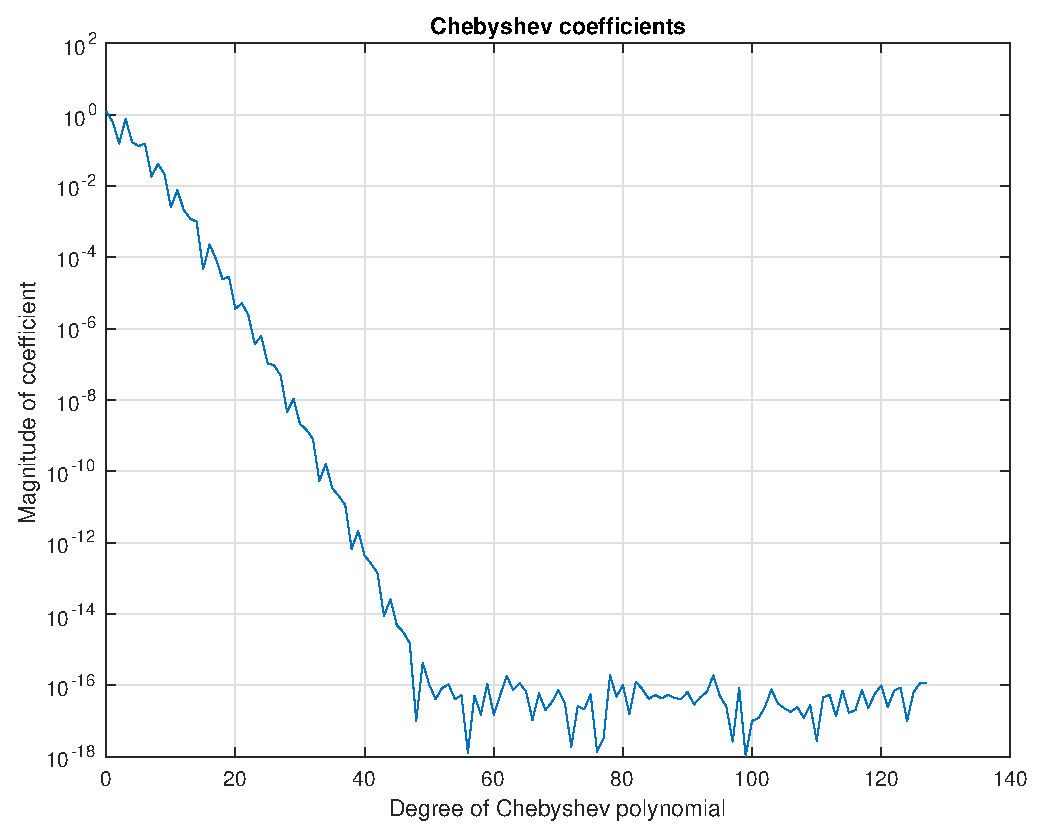
\includegraphics[scale = 0.5]{Chapter1/coeff_plot.eps}
\caption{Chebyshev coefficients for $f(x)=\exp \lp \sin \lp \pi x \rp \rp$.}
\label{Coeff_example}
\end{figure}

\section{Partition of unity formalism}
\label{PUM_FORM_SEC}
 Suppose we have an overlapping covering $\{ \Omega_k \}_{k=1}^N$ on a bounded region $\Omega$. A partition of unity is a collection of real valued functions $\{w_k(x)\}_{k=1}^N$ such that:
\begin{itemize}
\item $w_k(x)$ has support within $\Omega_k$,
\item each $w_k(x)$ is nonnegative,
\item $\forall x \in \Omega, \quad \sum_{k=1}^N w_k(x)=1$.
\end{itemize}
The functions $\{w_k(x)\}_{k=1}^N$ are called the \textit{weights} of the partition. Suppose now that $\Omega=[-1,1]$ and each $\Omega_k$ is an interval. We can use the partition of unity $\{w_k(x)\}_{k=1}^N$ to construct an approximating function. Suppose that for $m \geq 0$ we have a function $f \in C^{m}([-1,1])$, each weight $w_k(x)\in C^{m}([-1,1])$ and for each patch $\Omega_k$ we have an approximation $s_k(x)$ of $f(x)$. Then the function
\begin{equation}
\label{POUAPPROX}
s(x) = \sum_{k=1}^N w_k(x)s_k(x)
\end{equation}
can be used to approximate $f(x)$ and its derivatives \cite{wendland2004scattered}.

\begin{thm}
\label{PUMCON}
Suppose $f \in C^{m}([-1,1])$ and for each patch $\Omega_k$ we have a function $s_k(x)$ such that
$$ \|f^{(\alpha)}(x)-s_k^{(\alpha)}(x)\|_{L_{\infty}(\Omega_k)} \leq \varepsilon_k(\alpha) $$
for $\alpha \leq m$. Thus for $j\leq m$, if $s(x)$ is the approximation (\ref{POUAPPROX}) then
\begin{equation}
\left \|f^{(j)}(x)- s^{(j)}(x) \right \|_{L_{\infty}(\Omega_k)} \leq \sum_{k=1}^N\sum_{i=0}^j \binom{j}{i} \left \| w_k^{(j-i)}(x) \right \|_{L_{\infty}(\Omega_k)} \epsilon_k(i).
\end{equation}
\end{thm}
\begin{proof}
Since $\sum_{k=1} w_k(x)=1$, $\sum_{k=1} w_k(x)f(x)=f(x)$. Thus
\begin{equation}
\begin{aligned}
\frac{d^{j}}{d x^j}f(x)-\frac{d^{j}}{d x^j} \sum_{k=1}^N w_k(x)s_k(x) &= \frac{d^{j}}{d x^j} \sum_{k=1}^N w_k(x)(f(x)-s_k(x)) \\
&= \sum_{k=1}^N\sum_{i=0}^j \binom{j}{i} w_k^{(j-i)}(x) \lp f^{(i)}(x)-s_k^{(i)}(x) \rp.
\end{aligned}
\end{equation}
The result follows from here by the triangle inequality.
\end{proof}


\section{Convergence analysis}
\label{converge_sec}
In this section we consider a single interval partitioned into two overlapping parts, i.e.
$[-1,t]$,$[-t,1]$, where $t$ is the overlap parameter such that $0<t<1$. For the weights, we use Shepard's method \cite{shepard1968two} based on the compactly supported, infinitely differentiable shape function
\begin{align}
\psi(x) = \begin{cases}
\exp \lp  1 - \frac{1}{1-x^2}\rp & |x| < 1, \\
0 & |x| \geq 1.
\end{cases}
\end{align}
We define support functions
\begin{align}
\psi_{\ell}(x) = \psi \lp \frac{x+1}{1+t} \rp \quad \text{ and } \quad \psi_{r}(x) = \psi \lp \frac{x-1}{1+t} \rp ,
\end{align}
to construct the PU weight functions
\begin{align}
w_{\ell}(x) = \frac{\psi_{\ell}(x)}{\psi_{\ell}(x)+\psi_{r}(x)} \quad \text{and} \quad w_{r}(x) = \frac{\psi_{r}(x)}{\psi_{\ell}(x)+\psi_{r}(x)},
\label{PUW}
\end{align}
where $w_{\ell}(x),w_{r}(x)$ have support on the left and right intervals, respectively.

Suppose that $s_{\ell}(x),s_{r}(x)$ approximate $f(x)$ on $[-1,t]$, $[-t,1]$ respectively and are both infinitely smooth. Let
\begin{equation}
s(x) = w_{\ell}(x)s_{\ell}(x)+w_{r}(x)s_{r}(x),
\label{PUM2}
\end{equation}
where $s(x)$ is the partition of unity approximation. Following Theorem~\ref{PUMCON} we have for $x \in [-1,1]$ that
\begin{equation}
\begin{aligned}
\left | f(x)-s(x) \right | &= \left | w_{\ell}(x) \lp f(x) - s_{\ell}(x) \rp + w_{r}(x) \lp f(x) - s_{r}(x) \rp \right | \\
&\leq w_{\ell}(x) \left | f(x) - s_{\ell}(x) \right | + w_{r}(x) \left | f(x) - s_{r}(x) \right |.
\end{aligned}
\end{equation}
We conclude that
\begin{align}
\left \| f(x)-s(x) \right \|_{L_{\infty}[-1,1]} \leq \max \lp \left \| f(x)-s_{\ell}(x) \right \|_{L_{\infty}[-1,t]} , \left \| f(x)-s_{r}(x) \right \|_{L_{\infty}[-t,1]} \rp.
\label{POU_UP}
\end{align}
This implies that the Partition of unity Method (PUM) preserves the accuracy of its local approximants. We also have that $s(x)$ is infinitely smooth. For the first derivative we have
\begin{equation}
\begin{aligned}
\left | f'(x)-s'(x) \right | &\leq \left | w_{\ell}(x) \lp f'(x)-s_{\ell}'(x) \rp \right |+\left | w_{r}(x) \lp f'(x)-s_{r}'(x) \rp \right | \\
&+\left | w_{\ell
}'(x) \lp f(x)-s_{\ell}(x) \rp \right | +\left | w_{r}'(x) \lp f(x)-s_{r}(x) \rp \right |,
\end{aligned}
\end{equation}
giving us
\begin{equation}
\begin{aligned}
\left \| f'(x)-s'(x) \right \|_{L_{\infty}[-1,1]} &\leq \max \lp \left \| f'(x)-s_{\ell}'(x) \right \|_{L_{\infty}[-1,t]} , \left \| f'(x)-s_{r}'(x) \right \|_{L_{\infty}[-t,1]} \rp \\
&+\left \| w_{\ell}'(x) \right \|_{L_{\infty}[-t,t]} \left \| f(x)-s_{\ell}(x)\right \|_{L_{\infty}[-t,t]}\\ 
&+ \left \| w_{r}'(x) \right \|_{L_{\infty}[-t,t]} \left \| f(x)-s_{r}(x)\right \|_{L_{\infty}[-t,t]},
\end{aligned}
\label{diff_error}
\end{equation}
since the derivatives of the weights have support only on the overlap. For $t \ll 1$, the weights steepen to become nearly step functions. This causes the derivatives of the weights to be large in magnitude, resulting in an increase in the error for the derivative.

Since $w_{\ell}'(x)=-w_{r}'(x)$, from (\ref{diff_error}) we can infer
\begin{equation}
\begin{aligned}
\left \| f'(x)-s'(x) \right \|_{L_{\infty}[-1,1]} \leq \max \lp \left \| f'(x)-s_{\ell}'(x) \right \|_{L_{\infty}[-1,t]} , \left \| f'(x)-s_{r}'(x) \right \|_{L_{\infty}[-t,1]} \rp& \\
+\left \| w_{\ell}'(x) \right \|_{L_{\infty}[-t,t]} \max \lp \left \| f(x)-s_{\ell}(x)\right \|_{L_{\infty}[-t,t]}
, \left \| f(x)-s_{r}(x)\right \|_{L_{\infty}[-t,t]} \rp. &
\end{aligned}
\label{diff_error_2}
\end{equation}
We have that $x=0$ is a critical point of $w_{\ell}'(x)$ and for $t<0.4$ it can be shown that the maximum of $\left |w_{\ell}'(x) \right |$ occurs at $x=0$. Since
\begin{equation}
w_{\ell}'(0) = -\frac{(1+t)^2}{t^2 (2+t)^2},
\end{equation}
we can infer that $\left \| w_{\ell}'(x) \right \|_{L_{\infty}[-t,t]} = \Theta(t^{-2})$ as $t\to 0$. The norm of the Chebyshev differentiation operator is $\Theta(n^2)$ (for $n$ nodes), implying that the two terms on the right-hand side of (\ref{diff_error_2}) are balanced if $t^{-2}=\Theta(n^2)$, or equivalently $t = \Theta \lp \frac{1}{n} \rp$. A simple example of a split can be seen in Figure~\ref{ARCTAN}.

 
\begin{figure}[!htb]
\centering
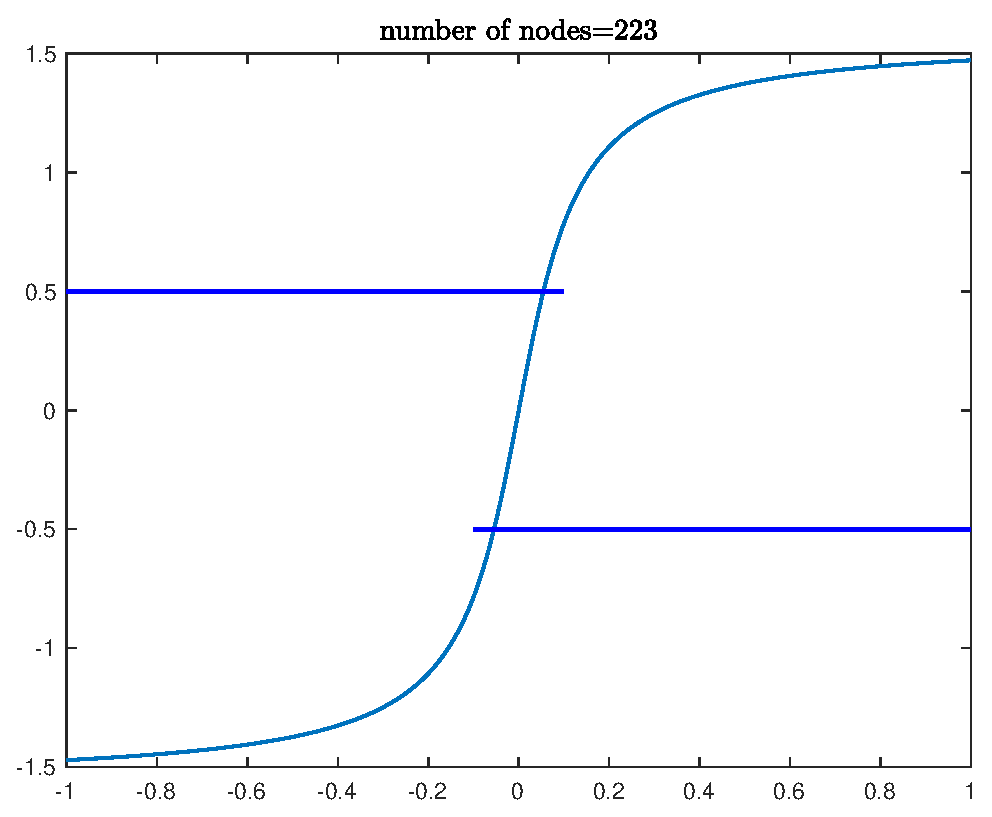
\includegraphics[scale = 0.5]{Chapter1/PUTANEXAMP.eps}
\caption{Plot of the PU approximation with overlap parameter $t=0.1$ for $f(x)=\arctan \lp x/0.1 \rp$, where the thick lines represent the domains of the left and right approximation. Here $\left \| f(x)-s(x) \right \|_{L_{\infty}[-1,1]}= 2.4 \mathrm{e}{-15}$ and $\left \| f'(x)-s'(x) \right \|_{L_{\infty}[-1,1]}= 1.7 \mathrm{e}{-13}$.}
\label{ARCTAN}
\end{figure}

\section{Recursive algorithm}
\label{PUM_recurse}
In order to allow for adaptation to specific features of $f(x)$, we next describe a recursive bisection algorithm that works similarly to Chebfun's splitting algorithm \cite{driscoll2014optimal} and to that of \cite{tobor2006reconstructing}. Suppose we want to construct a PU approximation $s_{[a,b]}(x)$ on the interval $[a,b]$ using Chebyshev interpolants on the patches. Our strategy is to cover $[a,b]$ with overlapping subdomains, on each of which $f$ is well-approximated by a Chebyshev polynomial, and using the binary tree recursively define a partition of unity approximation.

In this section we describe an adaptive procedure for obtaining the overlapping domains and individual approximations over them. The domains are constructed from recursive bisections of $[a,b]$ into nonoverlapping interverals, referred to as \emph{zones}. Given a zone $[\alpha,\beta]$, we extend it to a larger domain $[\bar{\alpha},\bar{\beta}]$ by fixing a parameter $t>0$, defining
\begin{equation}
  \label{eq:overlap1d}
  \delta_{j} =  \frac{\beta-\alpha}{2}(1+t),
\end{equation}
and then setting
\begin{equation}
  \bar{\alpha} = \max\{a,\beta-\delta\}, \quad \bar{\beta} = \min\{\alpha+\delta,b\}.
  \label{eq:zone_extend1d}
\end{equation}
In words, the zone is extended on both sides by an amount proportional, up to the boundary of the global domain $[a,b]$. 


% If $f(x)$ can be resolved by a Chebyshev interpolant $s(x)$ of length $\nmax$ on $[a,b]$ then
%\begin{align}
%s_{[a,b]}(x) = s(x).
%\end{align}
%Otherwise we split the interval into two overlapping domains and blend the results as in (\ref{PUM2}):
%\begin{align}
%s_{[a,b]}(x) = w_{\ell}(x)
%s_{\left [a,a+\delta \right ]}(x)+ w_{r}(x) s_{\left [b-\delta,b\right ]}(x),
%\end{align}
%where $w_{\ell},w_{r}$ are the PU weight functions defined in (\ref{PUW}) (but defined for $[a,b]$, and $\delta= (1+t) \lp \frac{a+b}{2} \rp$).

We define a binary tree $T$ with each node $\nu$ having the following properties:
\begin{itemize}
\item \textsf{domain}($\nu$):=the domain of the patch
\item \textsf{zone}($\nu$):=the zone of the patch
\item \child{0}($\nu$),\child{1}($\nu$):=respective left and right subtrees of $\nu$ (if split)
\item \weight{0}($\nu$),\weight{1}($\nu$):=respective left and right weights of $\nu$ (if split)
\item \textsf{interpolant}($\nu$):=Chebyshev interpolant on \textsf{domain}($\nu$) if $\nu$ is a leaf
\item \textsf{\textsf{values}}($\nu$):=values of the function we are approximating at the Chebyshev points of $\nu$.
\end{itemize}

For a node $\nu$ we recursively define the approximation on \textsf{domain}($\nu$) as
\begin{align}
s_{\nu}(x) = \weight{0}(\nu) s_{\text{\child{0}($\nu$)}}(x) + \weight{1}(\nu) s_{\text{\child{1}($\nu$)}}(x)
\end{align}
where approximations on leaves are defined to be Chebyshev polynomials. We prove in Theorem~\ref{PU_Proof} that this results in a partition of unity approximation. In Algorithm~\ref{alg2} we formally describe how we refine our splitting; the merge method is described in section~\ref{Merging_sec}. 

\begin{algorithm}[!h]
\caption{refine($\nu$,$f$,$\nmax$,$t$)}
\label{alg2}
\begin{algorithmic}
\IF{$\nu$ is a leaf and $f$ cannot be resolved by \textsf{interpolant}($\nu$)}
\STATE Define new nodes $\nu_0$, $\nu_1$.
\STATE $[a,b]$:=\textsf{domain}($\nu$)
\STATE $m = \frac{a+b}{2}$
\STATE \textsf{zone}(\child{0}($\nu$)) = $[b,m]$
\STATE \textsf{zone}(\child{1}($\nu$)) = $[m,a]$
\STATE \textsf{domain}(\child{0}($\nu$)), \textsf{domain}(\child{1}($\nu$)) are formed as in (\ref{eq:zone_extend1d})
\STATE \textsf{domain}($\nu$) = \textsf{domain}(\child{0}($\nu$)) $\cup$ \textsf{domain}(\child{1}($\nu$))
\STATE \child{0}($\nu$) := $\nu_0$
\STATE \child{1}($\nu$) := $\nu_1$
\STATE \weight{0}($\nu$),\weight{1}($\nu$):= weights in (\ref{PUW}) defined for \textsf{domain}($\nu_0$), \textsf{domain}($\nu_1$)
\ELSIF{$\nu$ is a leaf and $f(x)$ can be resolved by a Chebyshev \textsf{interpolant} with degree less than $\nmax$}
\STATE \textsf{interpolant}($\nu$):=minimum degree \textsf{interpolant} $f(x)$ can be resolved by \ARP 
as determined by Chebfun
\ELSE
\STATE refine(\child{0}($\nu$),$f$,$\nmax$,$t$)
\STATE refine(\child{1}($\nu$),$f$,$\nmax$,$t$)
\STATE \textsf{domain}($\nu$) = \textsf{domain}(\child{0}($\nu$)) $\cup$ \textsf{domain}(\child{1}($\nu$))
\STATE merge($\nu$,$\nmax$)
\ENDIF
\end{algorithmic}
\end{algorithm}

We first initialize the tree $T$ with a single node $\nu$ where \textsf{domain}($\nu$)=$[a,b]$. Next we repeatedly call the refine method until each leaf of $T$ has a Chebyshev interpolant that can resolve $f(x)$ with degree less than $\nmax$, as seen in Algorithm~\ref{alg2}. For a leaf $\nu$, we determine if a Chebyshev interpolant can resolve $f(x)$ using Chebfun's standardChop method with \textsf{values}($\nu$) (as described in Section~\ref{sec_cheb}). Using $T$ we can evaluate $s_{[a,b]}(x)$ recursively as demonstrated in Algorithm~\ref{alg3}. 

%\begin{algorithm}[!h]
%\caption{$T$=refine($\nmax$,$t$,$f(x)$)}
%\label{alg6}
%\begin{algorithmic}
%\STATE Define $T$ as a tree with a single node.
%\WHILE{$T$ has unresolved leaves}
%\STATE sample($T$,$f(x)$)
%\STATE splitleaves(root($T$),$\nmax$,$t$)
%\ENDWHILE
%\end{algorithmic}
%\end{algorithm}




\begin{algorithm}[!h]
\caption{v=eval($\nu$,$x$)}
\label{alg3}
\begin{algorithmic}
\IF{$\nu$ is a leaf}
\STATE $p$:=\textsf{interpolant}($\nu$)
\STATE v:= $p(x)$
\ELSE
\STATE $v_0,v_1$:=0

\STATE $w_0$:=\weight{0}($\nu$)
\STATE $w_1$:=\weight{1}($\nu$)
\FOR{$k=0,1$}
\IF{$x \in$ \textsf{domain}(\child{k}($\nu$))}
\STATE $v_k$:=eval(\child{k}($\nu$),$x$)
\ENDIF
\ENDFOR
\STATE v := $w_0(x)v_0 + w_1(x)v_1$
\ENDIF
\end{algorithmic}
\end{algorithm}

As a simple example, we approximate the function $f(x)=\arctan \lp \frac{x-0.25}{0.001} \rp$ with $n_{\max}=128$. In order to resolve to machine precision, a global Chebyshev interpolant on the interval $[-1,1]$ requires 25743 nodes while our method requires 412. Chebfun with non-overlapping splitting requires 381 nodes. Overlapping splittings will typically require more total nodes while offering the benefit of global smoothness. The result can be seen in Figure~\ref{ARCTAN2}.

\begin{figure}[!htb]
\centering
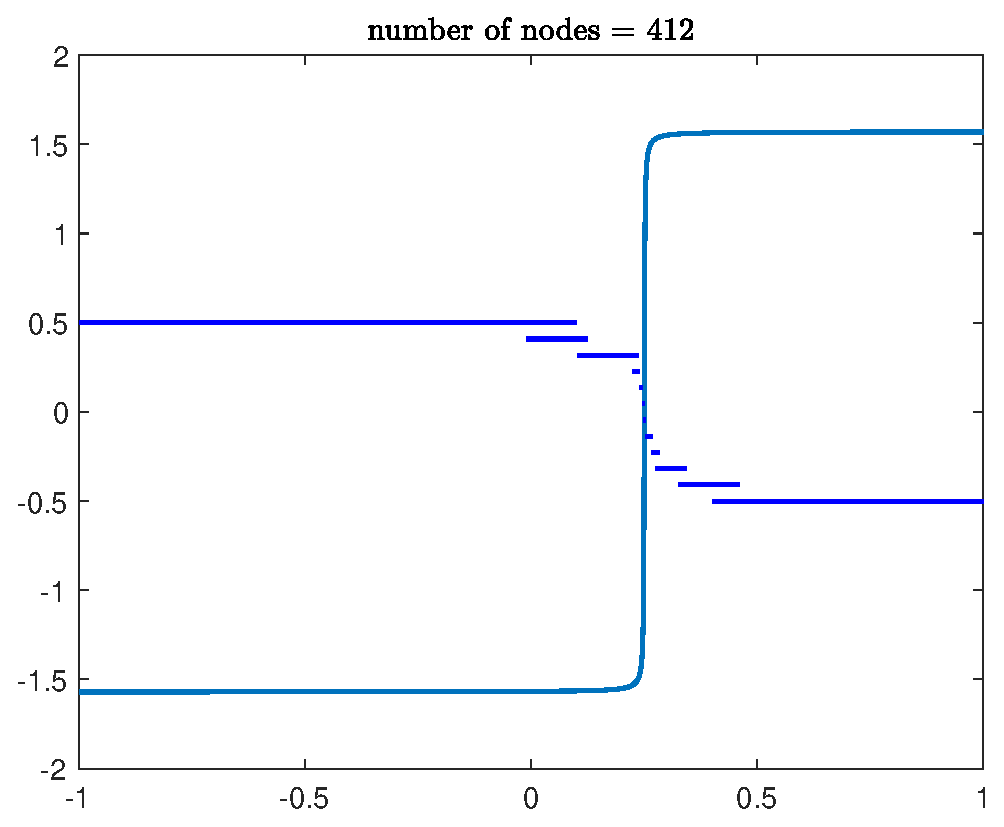
\includegraphics[scale = 0.5]{Chapter1/non_merging_example.eps}
\caption{Plot of the partition of unity approximation with overlap parameter $t=0.1$ for $f(x)=\arctan \lp (x-0.25)/0.001 \rp$, where the solid blue lines represent the patches.}
\label{ARCTAN2}
\end{figure}


We can deduce from (\ref{POU_UP}) that $s_{[a,b]}(x)$ will approximate $f(x)$. Moreover, our method implicitly creates a PU on the leaves of the tree through the product of the weights at each level.

\begin{thm}
Let an approximation $s_{[a,b]}(x)$ be as in (\ref{PUM2}). Then the tree that represents $s_{[a,b]}(x)$ implicitly defines a PU $\{w_k(x)\}_{k=1}^M$, where $w_k(x)$ has compact support over the $k$th leaf.
\label{PU_Proof}
\end{thm}
\begin{proof}
Suppose that on the domain $[a,b]$ we have PU's $\{w_{\ell k}(x)\}_{k=1}^{M_\ell}$, $\{w_{rk}(x)\}_{k=1}^{M_r}$ for the leaves of the left and right child respectively. We claim that
\begin{equation}
\{w_{\ell}(x) w_{\ell k}(x)\}_{k=1}^{M_\ell} \cup \{w_r(x) w_{r k}(x)\}_{k=1}^{M_r}
\label{UNPU}
\end{equation}
forms a PU over the leaves of the tree. We first observe that $w_{\ell}(x)w_{\ell k}(x)$ will have support in $\supp \lp w_{1k}(x) \rp$, the domain of the respective leaf. This is similarly true for $w_{r}(x)w_{r k}(x)$.


Next suppose that $x \in \sup \lp w_{\ell}(x)\rp \cap \, \sup \lp w_{r}(x)\rp^C$. Then $w_{\ell}(x)=1$ and $w_r(x)=0$, so
\begin{equation}
\sum_{k=1}^{M_\ell} w_{\ell}(x) w_{\ell k}(x)+ \sum_{k=1}^{M_r} w_{r}(x) w_{r k}(x) = \sum_{k=1}^{M_\ell} w_{\ell k}(x) = 1,
\end{equation}
since $\{w_{\ell k}(x)\}_{k=1}^{M_\ell}$ is a PU. This is similarly true if $x \in \sup \lp w_{\ell}(x)\rp^C \cap \sup \lp w_{r}(x)\rp$. Finally if $x \in \sup \lp w_{\ell}(x)\rp \cap \sup \lp w_{r}(x)\rp$ then
\begin{equation}
\begin{aligned}
\sum_{k=1}^{M_\ell} w_{\ell}(x) w_{\ell k}(x)+ \sum_{k=1}^{M_r} w_{r}(x) w_{r k}(x) &=  w_{\ell}(x) \sum_{k=1}^{M_\ell}  w_{\ell k}(x)+ w_{r}(x) \sum_{k=1}^{M_r} w_{r k}(x) \\
&= w_{\ell}(x)+w_{r}(x)=1.
\end{aligned}
\end{equation}
Thus by induction, we have that the product of weights through the binary tree for (\ref{PUM2}) implicitly creates a PU over the leaves.
\end{proof}


\subsection{Merging}
\label{Merging_sec}
As we create the tree we opportunistically merge leaves for greater efficiency. If a particular location in the interval requires a great deal of refinement, the recursive splitting essentially performs a binary search for that location (as was noted about Chebfun splitting in \cite{driscoll2014optimal}). The intermediate splits are not necessarily aiding with resolving the function; they are there just to keep the binary tree full. In Chebfun the recursive splitting phase is followed by a merging phase that discards counterproductive splits. We describe a similar merging operation here, but we allow these merges to take place whenever a leaf splits while its sibling does not, in order to keep the number of leaves from unnecessarily growing exponentially.

\begin{figure}[!htb]
\centering
\adjustbox{valign=t}{ 
\subfloat[Tree before merging. Here ${a_2<b_1}$ and ${a_{22}<b_{21}}$.]{
     \begin{forest}
for tree={circle,draw, l sep=20pt,,scale=0.98}
[ {$\begin{array}{c}
[a,b] \\
s_{[a,b]}(x)
\end{array}$}
    [ {$\begin{array}{c}
 [a,b_1]  \\
s_{[a,b_{1}]}(x) \\
 w_{\ell_1}(x)
\end{array}$},name=left_p]
    [ {{$\begin{array}{c}
    [a_2,b] \\
s_{[a_{2},b]}(x) \\
 w_{r_1}(x)
\end{array}$}} 
      [{$\begin{array}{c}
 [a_2,b_{21}] \\     
s_{[a_2,b_{21}]}(x) \\
 w_{\ell_2}(x)
\end{array}$},name=right_p] 
      [{$\begin{array}{c}
  [a_{22},b] \\    
s_{[a_{22},b]}(x) \\
 w_{r_2}(x)
\end{array}$}] 
  ] 
]
]
\draw[<->,dotted,thick] (right_p) to[out=north west,in=south] (left_p);
\end{forest}
   \label{TRM_1}
 }}\hfill
\adjustbox{valign=t}{ 
\subfloat[Tree after merging.]{
     \begin{forest}
for tree={circle,draw, l sep=20pt,scale=0.98}
[ {$\begin{array}{c}
[a,b]\\
s_{[a,b]}(x)
\end{array}$}
    [ {$\begin{array}{c}
 [a,b_{21}] \\   
s_{[a,b_{21}]}(x) \\
\hat{w}_{\ell_1}(x)
\end{array}$} ]
    [ {$\begin{array}{c}
[a_{22},b] \\    
s_{[a_{22},b] }(x) \\
\hat{w}_{r_1}(x)
\end{array}$} ] 
]
]
\end{forest}
   \label{TRM_2}
 }}
\caption{An example of how leaves are merged, where each node is labeled with its domain, PU approximation and weight.}
\label{Tree_merge}
\end{figure}

%\begin{figure}[!htb]
%\centering
%\adjustbox{valign=t}{ 
%\subfloat[Tree before merging. Here ${a_2<b_1}$ and ${a_{22}<b_{21}}$.]{
%     \begin{forest}
%for tree={circle,draw, l sep=20pt,,scale=0.98}
%[ {$\begin{array}{c}
%[a,b] \\
%s_{[a,b]}(x)
%\end{array}$}
%    [ {$\begin{array}{c}
% [a,b_1]  \\
%s_{[a,b_{1}]}(x) \\
% w_{\ell_1}(x)
%\end{array}$},name=left_p]
%    [ {{$\begin{array}{c}
%    [a_2,b] \\
%s_{[a_{2},b]}(x) \\
% w_{r_1}(x)
%\end{array}$}} 
%      [{$\begin{array}{c}
% [a_2,b_{21}] \\     
%s_{[a_2,b_{21}]}(x) \\
% w_{\ell_2}(x)
%\end{array}$},name=right_p] 
%      [{$\begin{array}{c}
%  [a_{22},b] \\    
%s_{[a_{22},b]}(x) \\
% w_{r_2}(x)
%\end{array}$}] 
%  ] 
%]
%]
%\draw[<->,dotted,thick] (right_p) to[out=north west,in=south] (left_p);
%\end{forest}
%   \label{TRM_1}
% }}\hfill
%\adjustbox{valign=t}{ 
%\subfloat[Tree after merging.]{
%     \begin{forest}
%for tree={circle,draw, l sep=20pt,scale=0.98}
%[ {$\begin{array}{c}
%[a,b]\\
%s_{[a,b]}(x)
%\end{array}$}
%    [ {$\begin{array}{c}
% [a,b_{21}] \\   
%s_{[a,b_{21}]}(x) \\
%\hat{w}_{\ell_1}(x)
%\end{array}$} ]
%    [ {$\begin{array}{c}
%[a_{22},b] \\    
%s_{[a_{22},b] }(x) \\
%\hat{w}_{r_1}(x)
%\end{array}$} ] 
%]
%]
%\end{forest}
%   \label{TRM_2}
% }}
%\caption{An example of how leaves are merged, where each node is labeled with its domain, PU approximation and weight.}
%\label{Tree_merge}
%\end{figure}

In Figure~\ref{Tree_merge} we illustrate how we merge leaves; the interval $[a,b_{1}]$ is merged with $[a_2,b_{21}]$. Here we decide to merge if $f(x)$ can be resolved with an interpolant with degree less than $\nmax$ on the interval $[a,b_{21}]$. For the new tree we define the left weight $\hat{w}_{\ell_1}(x)$ in Figure~\ref{Tree_merge} as
\begin{align}
\hat{w}_{\ell_1}(x) = \begin{cases} 
                1 & x<a_{22}, \\
                w_{\ell_2}(x) & \text{ otherwise.}        
\end{cases}
\label{pwe}
\end{align}
Since $w_{\ell_2}(x)=1$ for $x<a_{22}$, $\hat{w}_{\ell_1}(x)$ is smooth. For the right weight we use $\hat{w}_{r_1}(x) = w_{r_2}(x)$; these new weights form a PU. The PU approximation
\begin{align}
\hat{s}(x)=w_{\ell 1}(x) s_{[a,b_{1}]}(x)+w_{r 1}(x) s_{[a_2,b_{21}]}(x)
\end{align}
can be used to approximate  $f(x)$ on $[a,b_{21}]$ since $f(x)$ is resolved at the leaves. In this case $s_{[a,b_{21}]}(x)$ is computed from sampling $\hat{s}(x)$. If the degree of $s_{[a,b_{21}]}(x)$ after Chebfun's chopping is less than $\nmax$, we decide to merge. We explain in more detail the merging in Algorithm~\ref{alg5}; here extend($w(x)$,$[a,b]$) piecewise extends the weight $w(x)$ in $[a,b]$ as in (\ref{pwe}).  We show the results for merging in Figure~\ref{MERGE_EXAMPLE} with $f(x)=\frac{1}{x-1.001}$.

\begin{algorithm}[!h]
\caption{merge($\nu$,$\nmax$)}
\label{alg5}
\begin{algorithmic}
\IF{\child{0}($\nu$) and \child{0}(\child{1}($\nu$)) (child and grandchild of $\nu$) are leaves and both of the intervals of the leaves can be resolved on}
\STATE Define a new leaf $\nu_0$
\STATE $p_0(x)$:=\textsf{interpolant}(\child{0}($\nu$))
\STATE $p_1(x)$:=\textsf{interpolant}(\child{1}(\child{0}($\nu$)))
\STATE $w_0(x)$:= \weight{0}($\nu$)
\STATE $w_1(x)$:= \weight{1}($\nu$)
\STATE $\hat{s}(x)$:=$w_0(x)p_0(x)+w_1(x)p_1(x)$
\IF{$\hat{s}(x)$ can be resolved by a Chebyshev \textsf{interpolant} $p(x)$ with degree less than $\nmax$}
\STATE \textsf{domain}($\nu_0$):=\textsf{domain}(\child{0}($\nu$))$\cup$\textsf{domain}(\child{0}(\child{1}($\nu$)))
\STATE \textsf{interpolant}($\nu_0$):=$p(x)$
\STATE \textsf{points}($\nu_0$):=Chebyshev grid of length deg($p(x)$) on $[a_0,b_1]$
\STATE $\hat{w}_0(x)$:=  \weight{0}(\child{1}($\nu$))
\STATE $\hat{w}_1(x)$:=  \weight{1}(\child{1}($\nu$))
\STATE \weight{0}($\nu$):= extend($\hat{w}_0(x)$,\textsf{domain}($\nu_0$))
\STATE \weight{1}($\nu$):= $\hat{w}_1(x)$
\STATE \child{0}($\nu$):= $\nu_0$
\STATE \child{1}($\nu$):= \child{1}(\child{1}($\nu$))
\ENDIF
\ELSIF{\child{1}($\nu$) is a leaf and \child{1}(\child{0}($\nu$)) is a leaf (and exists)}
\STATE inv(merge($\nu$)) (i.e. apply the algorithm, except swap 0 and 1)
\ENDIF
\end{algorithmic}
\end{algorithm}

\begin{figure}[!htb]
\centering
\subfloat[Tree before merging.]{
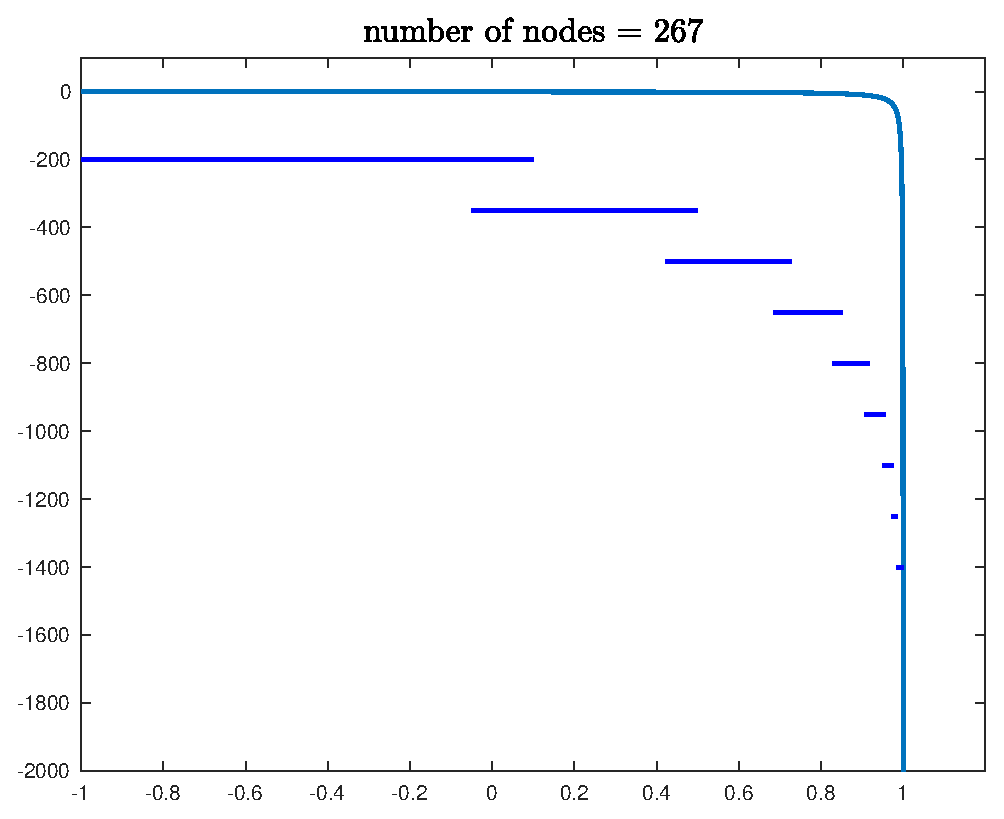
\includegraphics[scale = 0.35]{Chapter1/PUBEFORE_MERGE.eps}
   \label{MERGEB}
 }
\subfloat[Tree after merging.]{
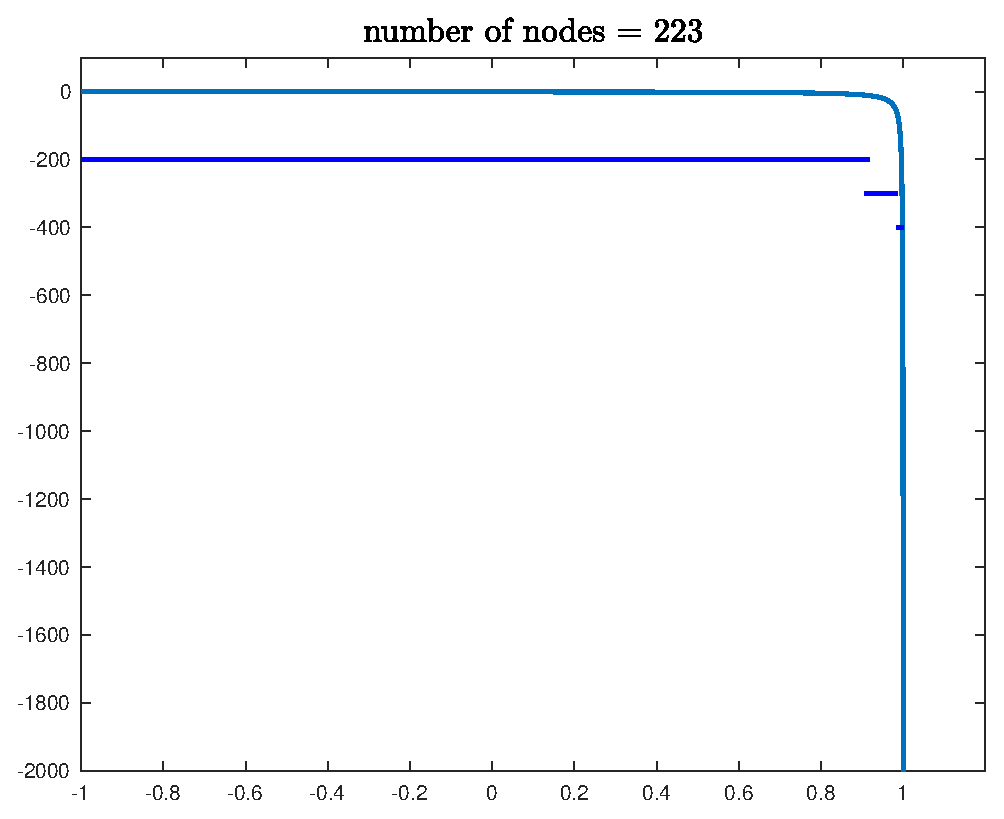
\includegraphics[scale = 0.35]{Chapter1/PUAFTER_MERGE.eps}
   \label{MERGEA}
 }
\caption{An example of how the PUM with $t=0.08$, $\nmax=128$ resolves $f(x)=\frac{1}{x-1.0005}$ without merging (a) and after merging (b).
}
\label{MERGE_EXAMPLE}
\end{figure}

\subsection{Differentiation matrices}
\label{PUM_matrix}
%Suppose we have a binary tree for the PUM approximation $s_{[a,b]}(x)$ for $f(x)$ as shown in Figure~\ref{PUMTREEDIFF}. We can construct differentiation matrices which evaluate the derivatives of $s_{[a,b]}(x)$  at the Chebyshev points of the leaves of the binary tree. 

Next we demonstrate how to construct a first derivative matrix; higher derivative matrices can be similarly constructed.  Suppose we have constructed a splitting represented with the tree $T$. For each node $\nu$ of the tree, we add the following methods:
\begin{itemize}
\item \textsf{points}($\nu$):= provides the Chebyshev points of the leaves of $\nu$
\item \textsf{leafpoints}($\nu$):= provides the Chebyshev points of $T$ in \textsf{domain}($\nu$) i.e. \newline $\text{\textsf{points}(root($T$))} \cap \text{\textsf{domain}($\nu$)}$
\item \textsf{pointindex}($\nu$):=gives the index of \textsf{points}($\nu$) with respect to the points of the parent of $\nu$ (if $\nu$ is a child)
\item \textsf{leafpointindex}($\nu$):=gives the index of \textsf{leafpoints}($\nu$) with respect to the leafpoints of the parent of $\nu$ (if $\nu$ is a child).
\end{itemize}



%Let $X$ be the set of Chebyshev points of the leaves of the entire tree (not just those of the root), $C$ be the set of Chebyshev points of the leaves, $X_{\ell} = X \cap [a,b-r]$ (the nodes only in the left patch), $X_{r} = X \cap [a+r,b]$ (the nodes only in the right patch), and $X_{c} = X \cap [b-r,a+r]$ (nodes in both patches).

%\begin{figure}[!htb]
%\centering
%\begin{forest}
%for tree={circle,draw, l sep=20pt}
%[ {$\begin{array}{c}
%s_{[a,b]}(x) \\
%D \\
%M \\
%C
%\end{array}$}
%    [ {$\begin{array}{c}
%s_{\left [a,a+r \right ]}(x) \\
%w_{\ell}(x) \\
%D_{\ell} \\
%M_{\ell} \\
%C_{\ell} \\
%\end{array}$} ]
%    [ {$\begin{array}{c}
%s_{[b-r,b]}(x) \\
%w_{r}(x) \\
%D_{r} \\
%M_{r} \\
%C_{r}
%\end{array}$} ] 
%]
%]
%\end{forest}

%\caption{The PUM approximation $s_{[a,b]}(x)$ is represented as a tree rooted at $[a,b]$; the diameter $r=(1+t) \frac{a+b}{2}$, where $t$ is the overlap parameter. Each node has its respective approximate, weight function, differentiation matrix,interpolation matrix and Chebyshev points for all its leaves (shown in that order).}
%\label{PUMTREEDIFF}
%\end{figure}
Let $[\alpha,\beta]=\text{\textsf{domain}($\nu$)}$. We want to construct matrices $M,D$ such that 
\begin{equation}
\begin{aligned}
M \left . f(x) \right |_{\text{\textsf{points}($\nu$)}} &= \left . s_{[\alpha,\beta]}(x) \right |_{\text{\textsf{leafpoints}($\nu$)}}, \\
D \left . f(x) \right |_{\text{\textsf{points}($\nu$)}} &= \left . \frac{d}{dx} s_{[\alpha,\beta]}(x) \right |_{\text{\textsf{leafpoints}($\nu$)}}.
\end{aligned}
\end{equation}

Let $I_k = \text{\textsf{domain}(\child{k}($\nu$))}$, $w_k(x)=\text{\weight{k}($\nu$)}$ for $k=0,1$. Then
\begin{equation}
\begin{aligned}
\left . s_{[\alpha,\beta]}(x) \right |_{\text{\textsf{leafpoints}($\nu$)}} &= \sum_{k=0}^1 \left . w_k(x) s_{I_k}(x) \right |_{\text{\textsf{leafpoints}($\nu$)}}, \\
\left . \frac{d}{dx} s_{[\alpha,\beta]}(x) \right |_{\text{\textsf{leafpoints}($\nu$)}} &= \sum_{k=0}^1 \lp \left . w_k(x)  \frac{d}{dx} s_{I_k}(x) + \frac{d}{dx} w_k(x)  s_{I_k}(x) \rp \right |_{\text{\textsf{leafpoints}($\nu$)}} .
\end{aligned}
\label{sum_eval}
\end{equation}
Thus we can recursively build up the differentiation matrix through the tree $T$. Due to the support of the weights, for each term in (\ref{sum_eval}) we only need evaluate the approximation $s_{I_k}(x)$ (or its derivative) for $\text{\textsf{leafpoints}($\nu$)} \cap I_k$, i.e. \textsf{leafpoints}(\child{k}($\nu$)). We describe how to construct the differentiation recursively in Algorithm~\ref{alg4}, using MATLAB notation for matrices. At each leaf the interpolation matrix $M$ has entries given by the barycentric interpolation formula based on second-kind Chebyshev points, as produced by the Chebfun command {\tt barymat} \cite{driscoll2015rectangular}.

\begin{algorithm}
\caption{[$M,D$]=diffmatrix($\nu$)}
\label{alg4}
\begin{algorithmic}
\IF{$\nu$ is a leaf}
\STATE $M$:= the Chebyshev barycentric matrix from \textsf{points}($\nu$) to \textsf{\textsf{leafpoints}}($\nu$)
\STATE $D_x$:= Chebyshev differentiation matrix with grid \textsf{points}($\nu$).
\STATE $D$:=$M D_x$.
\ELSE
\STATE $M,D$:=zeros(length(\textsf{leafpoints}($\nu$)),length(\textsf{points}($\nu$)))
\FOR{$k=0,1$}
\STATE [$M_k$,$D_k$]:= diffmatrix(\child{k}($\nu$))
\STATE $M$(\textsf{leafpointindex}(\child{k}($\nu$)),\textsf{pointindex}(\child{k}($\nu$))) = \WRP \text{diag} $\lp \left . w_k \right |_{\text{\textsf{leafpoints}(\child{k}($\nu$))}} \rp$*$M_k$;
\STATE $D$(\textsf{leafpointindex}(\child{k}($\nu$)),\textsf{pointindex}(\child{k}($\nu$))) = \WRP \text{diag} $\lp \left . w_k \right |_{\text{\textsf{leafpoints}(\child{k}($\nu$))}}  \rp$*$D_k$+ \WRP \text{diag} $\lp \frac{d}{dx} \left . w_k \right |_{\text{\textsf{leafpoints}(\child{k}($\nu$))}} \rp$*$M_k$;
\ENDFOR
\ENDIF
\end{algorithmic}
\end{algorithm}

For $x \in [\alpha,\beta]$ we only need to evaluate the local approximations for the patches $x$ belongs to; this implies that the differentiation matrices will be inherently sparse. For example, Figure~\ref{SPARSE_DX} shows the sparsity of the first derivative matrix for the tree generated in Figure~\ref{ARCTAN2}. In this case, we have a sparsity ratio of around 76\%.

\begin{figure}[!htb]
\centering
\includegraphics[scale = 0.5]{Chapter1/diff_sparse2.eps}
\caption{Sparsity of the first derivative matrix for the tree generated for Figure~\ref{ARCTAN2}.}
\label{SPARSE_DX}
\end{figure}

\section{PUM for boundary-value problems}
\label{PUM_BVP_SEC}
Our method can be applied to solve linear and nonlinear boundary-value problems. For instance, consider a simple Poisson problem with zero boundary conditions:
\begin{equation}
\begin{aligned}
&u''(x) = f(x) \text{ for }-1<x<1 \\
&u(-1)=0, u(1)=0.
\end{aligned}
\label{simp_pois}
\end{equation}
Suppose that we have differentiation and interpolation matrices $D_{xx}$ and $M$ from section~\ref{PUM_matrix}, $X$ is the set of Chebyshev points over all the leaves, and that $X_I$, $X_B$ are the respective interior and boundary points of $X$. Let $E_{I}$ and $E_{B}$ be the matrices that map a vector to its subvector for the interior and boundary indices respectively. Let $F$ be the vector of values used for the local interpolants (i.e. if we had only two leaves whose interpolants used values $F_1,F_2$, we set $F = [F_1^T  F_2^T]^T$). In order to find a PUM approximation $s(x)$ that approximates (\ref{simp_pois}) we find $F$ by solving the following linear system:
\begin{equation}
\begin{bmatrix}
E_{I} D_{xx} \\[1mm] 
 E_{B} M
\end{bmatrix}
\begin{bmatrix}
E_{I} F \\[1mm]
E_{B} F
\end{bmatrix}
=
\begin{bmatrix}
\left . f \right |_{X_I} \\[1mm]
0 \\ 
\end{bmatrix}.
\label{PUM_lin_system}
\end{equation}

Algorithm~\ref{BVP_solve} builds an adaptive solution for the BVP. We first construct a PU approximation $s(x)$ by solving the discretized system in (\ref{PUM_lin_system}). Sampling with $s(x)$, we use Algorithm~\ref{alg2} to determine if the solution is refined and split leaves that are determined to be unrefined. Here we also allow merging for a node with resolved left and right leaves (i.e., the left and right leaves can be merged back together).

\begin{algorithm}
\caption{$T$=refineBVP($\nmax$,$t$,BVP)}
\label{alg7}
\begin{algorithmic}
\STATE Define $T$ as a tree with a single node with the domain of the BVP.
\WHILE{$T$ has unrefined leaves}
\STATE Find values for the interpolants $F$ of the leaves of $T$ by solving a discretized \ARP system defined by the interpolation and differentiation matrices of $T$.
\STATE sample($T$,$F$) 
\STATE $s(x) = \text{eval}(\text{root}(T),x)$ (the PU approximation)
\STATE sample($T$,$s(x)$)
\STATE refine(root($T$),$\nmax$,$t$)
\ENDWHILE
\end{algorithmic}
\label{BVP_solve}
\end{algorithm}

\subsection{BVP example}
\label{BVP_SEC}
%We first solve
%\begin{equation}
%-\varepsilon u''(x)+u(x)=\sin(16 e^x), \quad u(-1)=u(1)=0
%\end{equation}
%for $\varepsilon \ll 1$; this is a singular perturbed problem with boundary layers of width $O(\varepsilon \log(1/\varepsilon))$ \cite{madden2003uniformly}. The tolerance we use for Chebfun's chopping method is $10^{-11}$ (due to the ill conditioning of the problem, a higher accuracy is difficult to achieve). We sample the residual of the ODE at 10000 points and record the maximum. We show the results for $\varepsilon^2$ between $10^{-6}$ and $10^{-12}$ in Table~\ref{Lin_results}.
%
%
%\begin{table}[!htb]
%\centering
%\caption{Summary of PUM results for the BVP \deleted{(\ref{PUM_lin_system})} \added{(\ref{simp_pois})}. }
%\label{Lin_results}
%\begin{tabular}{c|ccc}
%\hline
%$\varepsilon^2$ & \# of solves & total nodes & max residual \\ \hline
%$10^{-6}$       & 5            & 275         & 2.0744e-10   \\ \hline
%$10^{-8}$       & 9            & 275        & 3.8985e-08   \\ \hline
%$10^{-10}$      & 14           & 260         & 4.3393e-07   \\ \hline
%$10^{-12}$      & 16           & 255         & 9.1689e-07   \\ \hline
%\end{tabular}
%\end{table}
%
%\begin{figure}[!htb]
%\centering
%\subfloat[Solution with subintervals plotted.]{
%\includegraphics[scale = 0.35]{lin_plot.eps}
%   \label{LIN_EXAMPLEA}
% }
%\subfloat[Plot of the residual.]{
%\includegraphics[scale = 0.35]{lin_residual.eps}
%   \label{LIN_EXAMPLEB}
% }
%\caption{Numerical solution and residual for the BVP (\ref{PUM_lin_system}) with $\varepsilon^2=10^{-8}$.
%}
%\label{LIN_EXAMPLE}
%\end{figure}

We solve the stationary Burgers equation on the interval $[0,1]$ with Robin boundary conditions \cite{reyna1995exponentially}:
\begin{equation}
\begin{aligned}
&\nu u''(x)-u(x)u'(x)=0 \\
&\nu u'(0)-\kappa(u(0)-\alpha)=0 \\
&\nu u'(1)+\kappa(u(1)+\alpha)=0
\end{aligned}
\label{PUM_nlin_system}
\end{equation}
which has nontrivial solution
\begin{equation}
u(x)=-\beta \tanh \lp \frac{1}{2} \beta \nu^{-1} \lp x-\frac{1}{2} \rp \rp
\label{true_sol}
\end{equation}
where $\beta$ satisfies
\begin{equation}
-\frac{1}{2} \beta^2 \text{sech}^2 \lp \frac{1}{4} \beta \nu^{-1} \rp+\kappa \left [ \alpha-\beta \text{tanh} \lp \frac{1}{4} \beta \nu^{-1} \rp \right ]=0.
\end{equation}


We choose $\nu=5 \times 10^{-3},\alpha=1$, and $\kappa=2$. We use {\tt fsolve} in MATLAB to solve the BVP, supplying the Jacobian of the discretized nonlinear system. Starting with a linear guess $u(x)=0$, we update the solution from the latest solve (i.e. if the solution $s(x)$ from Algorithm~\ref{BVP_solve} is determined to be unresolved, we use it as the next initial guess). For this problem we set the Chebfun chopping tolerance to $10^{-10}$. Our solution was resolved to the tolerance we set after four nonlinear solves; as seen in Figure~\ref{NLIN_EXAMPLE}, the final approximation had 234 nodes and the absolute error was less than $10^{-4}$ as seen in Figure~\ref{NLIN_EXAMPLE}. On a machine with processor 2.6 GHz Intel Core i5, the solution was found in 1.3 seconds.

\begin{figure}[!htb]
\centering
\subfloat[Solution with subintervals plotted.]{
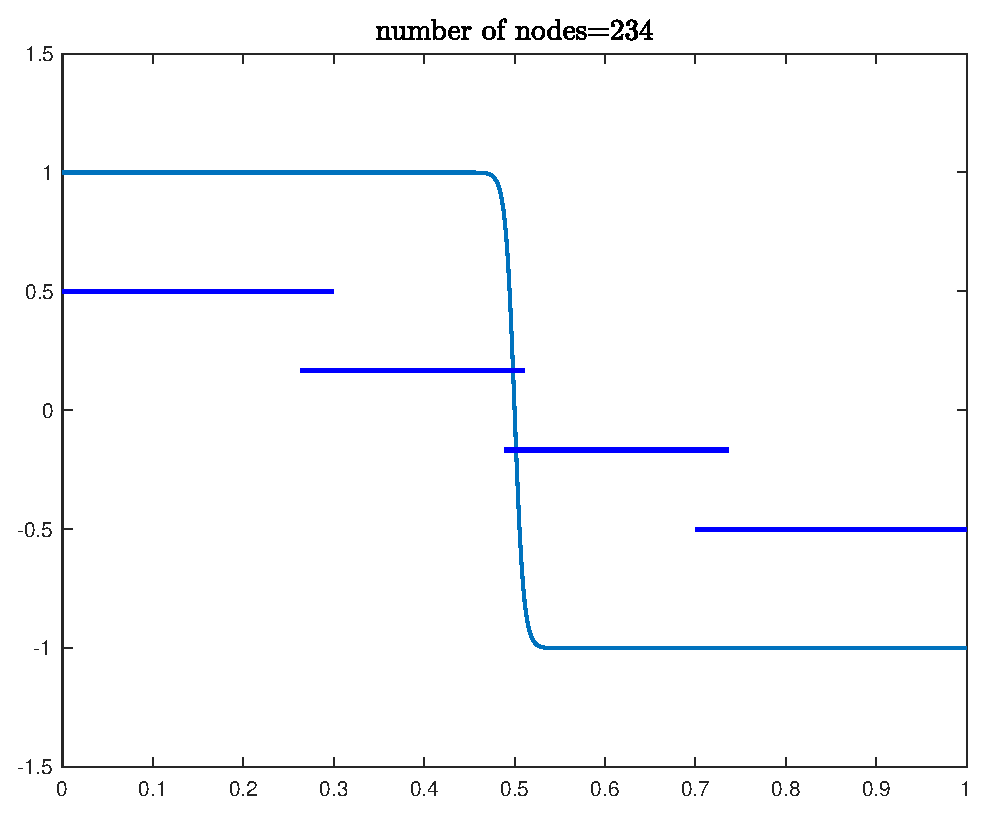
\includegraphics[scale = 0.35]{Chapter1/non_lin_plot.eps}
   \label{NLIN_EXAMPLEA}
 }
\subfloat[Plot of the error.]{
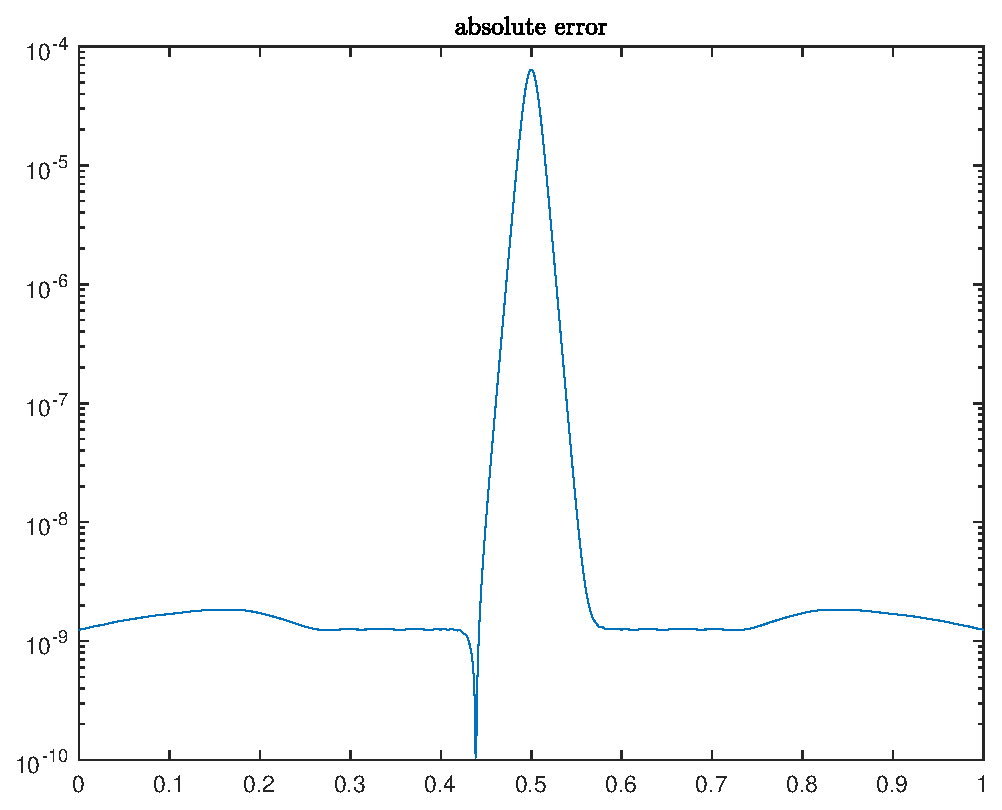
\includegraphics[scale = 0.35]{Chapter1/non_lin_residual.eps}
   \label{NLIN_EXAMPLEB}
 }
\caption{Numerical solution using the PU method and residual for the BVP (\ref{PUM_nlin_system}) with $\nu=5 \times 10^{-3}$, $t=0.1$, and $\nmax = 128$.}
\label{NLIN_EXAMPLE}
\end{figure}

We preformed a similar experiment but instead used global Chebyshev interpolants. We adapt by increasing the degree of the polynomial from $n$ to $\text{floor}(1.5 n)$, starting with $n=128$. We stop when we have a solution that is refined to the tolerance $10^{-10}$ (same as before). Both the solution and residual are in Figure~\ref{GNLIN_EXAMPLE}; here we have the absolute error is higher at 1.8e-2. The solution took 3.2 minutes on the same machine. There are two main reasons why the global solution performs much slower. First, in order to resolve the true solution with the tolerance $10^{-10}$, the global Chebyshev solution requires 766 nodes versus 234 for the PU approximation. Secondly, when adapting with the PUM, if a leaf is determined to be refined, the number of nodes is reduced as dictated in Algorithm~\ref{alg2} and the leaf is not split in further iterations. This keeps the total number of nodes lower while adapting.
 

\begin{figure}[!htb]
\centering
\subfloat[Numerical solution.]{
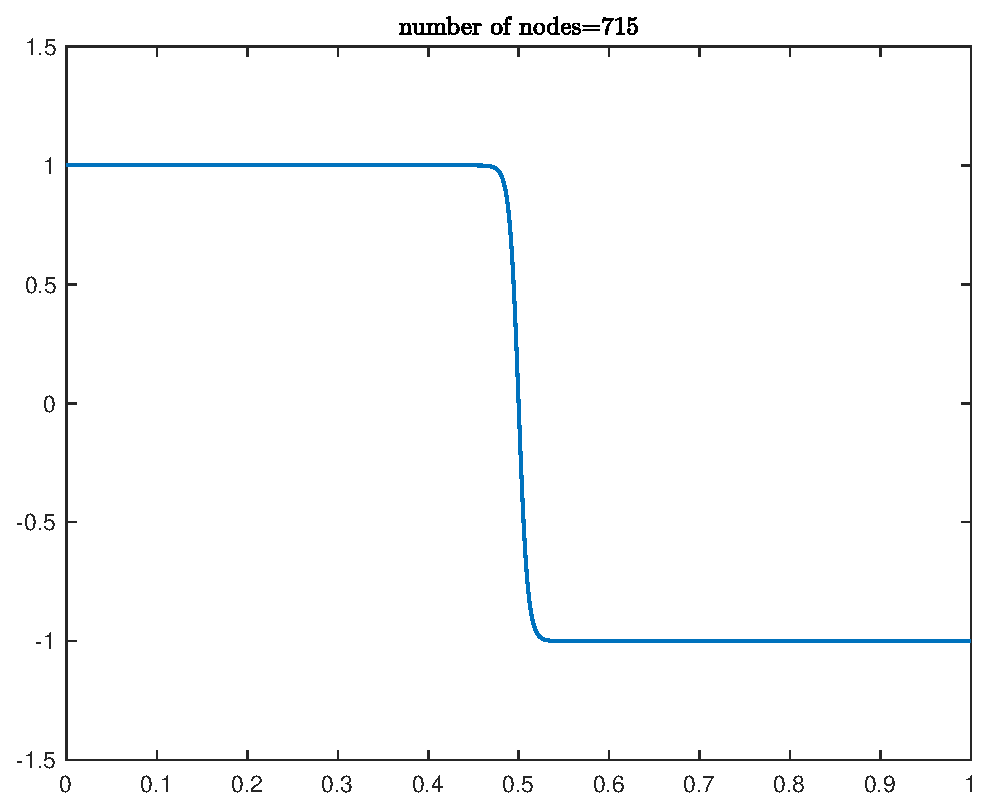
\includegraphics[scale = 0.35]{Chapter1/globalburger.eps}
   \label{GNLIN_EXAMPLEA}
 }
\subfloat[Plot of the error.]{
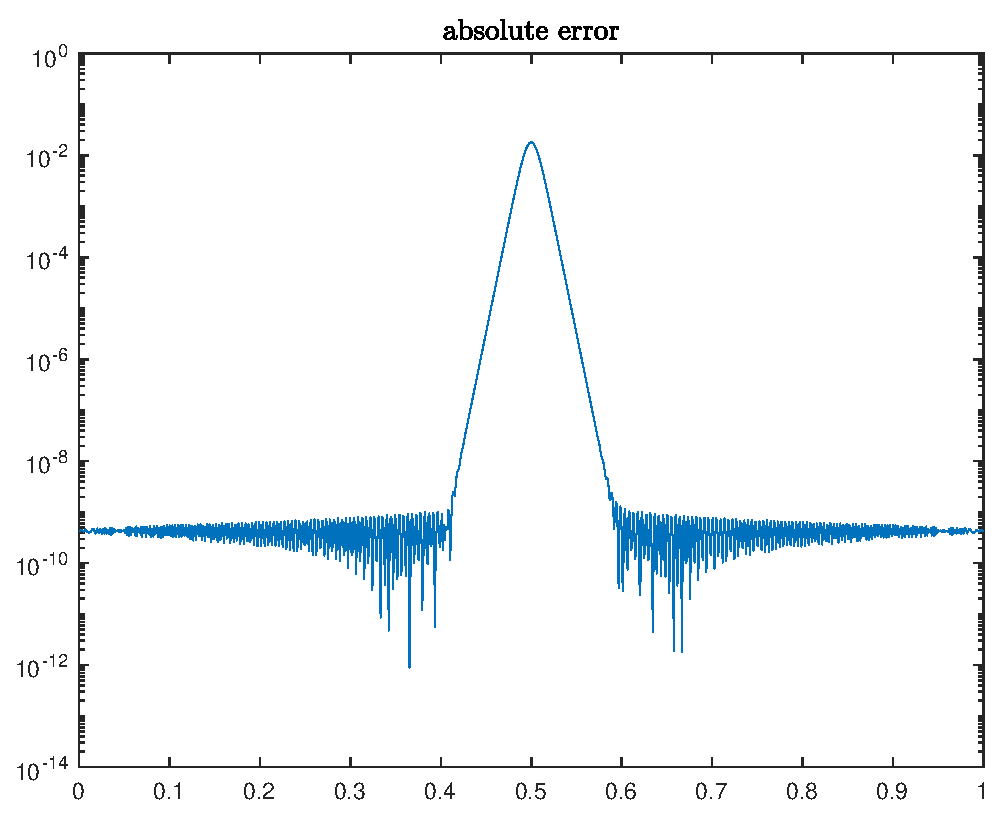
\includegraphics[scale = 0.35]{Chapter1/globalburgererr.eps}
   \label{GNLIN_EXAMPLEB}
 }
\caption{Numerical solution using the global Chebyshev method and residual for the BVP (\ref{PUM_nlin_system}) with $\nu=5 \times 10^{-3}$.
}
\label{GNLIN_EXAMPLE}
\end{figure}

\section{Discussion}
Our method offers a simple way to adaptively construct infinitely smooth approximations of functions that are given explicitly or that solve BVPs. By recursively constructing the PU weights with the binary tree, we avoid the need to determine the neighbors of each patch (as would be needed with the standard Shepard's PU weights). While this is not a serious issue in one dimension, the complexity of how the patches overlap increases with higher dimension. For example, in 2D we could build a similar method on a box where we use tensor product Chebyshev approximations. We would refine by splitting the box into two overlapping parts (either in $x$ or $y$) and recursively build a binary tree. We similarly would define partition of unities for each of the splits. If we used infinitely smooth weights at the splits, the 2D PU approximation will be infinitely smooth as well.


Our method leaves room for improvement. For instance, while merging helps reduce the number of nodes, in cases where we have a singularity right above the split the PU method over-resolves in the overlap; this can be seen in Figure~\ref{ARCTAN2}. The source of the problem is that patches may be adjacent in space but not in the tree. This could be resolved by a more robust merging algorithm. Alternatively we could determine an optimal splitting location through a Chebyshev-Pad\'{e} approximation as in \cite{driscoll2014optimal}, but the PU adds a layer of complexity since we must optimize not just for the splitting location but the size of the overlap.

Additionally it is possible to construct weights that are not $C^{\infty}$ but have smaller norms in their derivatives. For instance,
\begin{equation}
\begin{aligned}
w_{\ell}(x) &= \begin{cases}
1 & x \leq -t \\
\frac{1}{4t^3} x^3 - \frac{3}{4 t} x+\frac{1}{2} & -t\leq x \leq t \\
0 & x>t
 \end{cases} \\
 w_{r}(x) &= 1-w_{\ell}(x)
\end{aligned}
\end{equation}
defines a $C^1[-1,1]$ piecewise cubic partition of unity, where $\| w_{\ell}'(x)\|_{\infty} = \frac{3}{4t}$. If a BVP requires higher smoothness, we could similarly construct a higher degree polynomial for the weights.    % This file (chap1.tex) contains the text
                   % for Chapter 1.
                   
\chapter{An adaptive partition of unity method for multivariate Chebyshev polynomial approximations}
\label{pu_nd}

\section{Introduction}
\label{sec:introduction}

%A distinctive and powerful mode of scientific computation has emerged recently in which mathematical functions are represented by high-accuracy numerical analogs, which are then manipulated or analyzed numerically using a high-level toolset~\cite{Trefethen2015}. The most prominent example of this style of computing is the open-source Chebfun project~\cite{battles2004extension,Driscoll2014}. Chebfun, which is written in MATLAB, samples a given piecewise-smooth univariate function at scaled Chebyshev nodes and automatically determines a Chebyshev polynomial interpolant for the data, resulting in an approximation that is typically within a small multiple of double precision of the original function. This approximation can then be operated on and analyzed with algorithms that are fast in both the asymptotic and real-time senses. Notable operations include rootfinding, integration, optimization, solution of initial- and boundary-value problems, eigenvalues of differential and integral operators, and solution of time-dependent PDEs.

%Townsend and Trefethen extended the 1D Chebfun algorithms to 2D functions over rectangles in Chebfun2~\cite{townsend2013extension,Townsend2014}, which uses low-rank approximations in an adaptive cross approximation. The construction and manipulation of 2D approximations is suitably fast for a wide range of smooth examples. Most recently, Hashemi and Trefethen created an extension of Chebfun called Chebfun3 for 3D approximations on hyperrectangles using low-rank ``slice--Tucker'' decompositions~\cite{Hashemi2017}. The range of functions that Chebfun3 can cope with in a reasonable interactive computing time is somewhat narrower than for Chebfun2, as one would expect.

One aspect of the low-rank approximations used by Chebfun2 and Chebfun3 is that they are highly anisotropic. That is, rotation of the coordinate axes can transform a rank-one or low-rank function into one with a much higher rank, greatly increasing the time required for function construction and manipulations. This issue is considered in detail in~\cite{trefethen2017cubature}. 

%An alternative to Chebfun and related projects ported to other languages is sparse grid interpolation. Here one uses linear or polynomial interpolants on hierarchical Smolyak grids. Notable examples of software based on this technique are the Sparse Grid Interpolation Toolbox~\cite{Klimke2005} and the Sparse Grids Matlab Kit~\cite{Back2011}. An advantage of these packages is that they are capable of at least medium-dimensional representations on hyperrectangles. However, they seem to be less focused on high-accuracy approximation for a wide range of functions, and they are less fully featured than the Chebfun family. These methods are also highly nonisotropic.

In this chapter we propose decomposing a hyperrectangular domain by adaptive, recursive bisections in one dimension at a time, generalizing earlier work in one dimension \cite{Aiton2018}. The resulting subdomains are defined to be overlapping, and on each we employ simple tensor-product Chebyshev polynomial interpolants. In order to define a global smooth approximation, we use a partition of unity to blend together the subdomains. This allows the approximation to capture highly localized function features while remaining computationally tractable.

Our use of an adaptive decomposition allows us to approximate on such domains with great flexibility. If a base subdomain is hyperrectangular, we proceed with a tensor-product interpolation for speed, but if its intersection with the global domain is nonrectangular, we can opt for a different representation. We need not be concerned with having a very large number of degrees of freedom in any local subproblem, since further subdivision is available, so the local algorithm need not be overly sophisticated. 


The adaptive construction of function approximations is based on binary trees, as explained in section~\ref{sec:construction}. In section~\ref{sec:operations} we describe fast algorithms for evaluation, arithmetic combination, differentiation, and integration of the resulting tree-based approximations. Numerical experiments over hyperrectangles in section~\ref{sec:numerical_experiments} demonstrate that the tree-based approximations exhibit far less anisotropy than do Chebfun2 and Chebfun3. Our implementation is faster than Chebfun2 and Chebfun3 on all tested examples---sometimes by orders of magnitude---except for examples of very low rank, for which all the methods are acceptably fast. In section~\ref{sec:general-domain} we describe and demonstrate approximation on nonrectangular domains using a simple linear least-squares approximation by the tensor-product Chebyshev basis. While these results are preliminary, we think they show enough promise to merit further investigation. 



\section{Adaptive construction}
\label{sec:construction}

Let $\Omega = \{ \vect{x} \in \R^d: x_i \in [a_i,b_i], i=1,\ldots,d\}$ be a hyperrectangle, and suppose we wish to approximate $f:\Omega \to \R$. Our strategy is to cover $\Omega$ with overlapping subdomains, on each of which $f$ is well-approximated by a multivariate polynomial, and use a partition of unity to construct a global approximation. We defer a description of the partition of unity scheme to section~\ref{sec:operations}. In this section we describe an adaptive procedure for obtaining the overlapping domains and individual approximations over them. 

The domains are constructed from recursive bisections of $\Omega$ into nonoverlapping hyperrectangular \emph{zones}. Given a zone $\prod_{j=1}^d [\alpha_{j},\beta_{j}]$, we extend it to a larger domain $\prod_{j=1}^d [\bar{\alpha}_{j},\bar{\beta}_{j}]$ by fixing a parameter $t>0$, defining
\begin{equation}
  \label{eq:overlap}
  \delta_{j} =  \frac{\beta_{j}-\alpha_{j}}{2}(1+t),\quad j=1,\ldots,d,
\end{equation}
and then setting
\begin{equation}
  \bar{\alpha}_{j} = \max\{a_j,\beta_{j}-\delta_{j}\}, \quad \bar{\beta}_{j} = \min\{\alpha_{j}+\delta_{j},b_j\}.
  \label{eq:zone_extend}
\end{equation}
In words, the zone is extended on all sides by an amount proportional to its width in each dimension, up to the boundary of the global domain $\Omega$. 


We define a binary tree $\ct$ with each node $\nu$ having the following properties:
\begin{itemize}
\item \prop{zone}{$\nu$}: zone associated with $\nu$
\item \textsf{domain}($\nu$): domain associated with $\nu$
\item \textsf{isdone}($\nu$): $n$-vector of boolean values, where $\textsf{isdone}_j$ indicates whether the domain is determined to be sufficiently resolved in the $j$th dimension
\item \child{0}($\nu$),\child{1}($\nu$): left and right subtrees of $\nu$ (empty for a leaf)
\item \textsf{splitdim}($\nu$): the dimension in which $\nu$ is split (empty for a leaf)
\end{itemize}

\noindent A leaf node has the following additional properties:
\begin{itemize}
\item \textsf{grid}($\nu$): tensor-product grid of Chebyshev 2nd-kind points mapped to \prop{domain}{$\nu$}
\item \textsf{values}($\nu$): function values at \textsf{grid}($\nu$)
\item \textsf{interpolant}($\nu$): polynomial interpolant of \textsf{values}($\nu$) on \textsf{grid}($\nu$)
\end{itemize}

\noindent If $\nu$ is a leaf, its domain is constructed by extending \prop{zone}{$\nu$} as in~(\ref{eq:zone_extend}). Otherwise, \prop{domain}{$\nu$} is the smallest hyperrectangle containing the domains of its children. 

Let $f$ be the scalar-valued function on $\Omega$ that we wish to approximate. A key task is to compute, for a given leaf node $\nu$, the polynomial \textsf{interpolant}($\nu$), and determine whether $f$ is sufficiently well approximated on \textsf{domain}($\nu$) by it. First we sample $f$ at a Chebyshev grid of size $\nmax^d$ on \textsf{domain}($\nu$). This leads to the interpolating polynomial
\begin{equation}
  \label{eq:full-interp}
  \tilde{p}(\vect{x}) = \sum_{i_1=0}^{\nmax-1} \cdots \sum_{i_d=0}^{\nmax-1}  C_{i_1,\ldots,i_d} T_{i_1}(x_1)\cdots T_{i_d}(x_d),
\end{equation}
where the coefficient array $C$ can be computed by FFT in $\bigo(\nmax^d \log \nmax)$ time~\cite{mason2002chebyshev}. Following the practice of Chebfun3t \cite{Hashemi2017}, for each $j=1,\ldots,d$, we define a scalar sequence $\gamma^{(j)}$ by summing $|C_{i_1,\ldots,i_d}|$ over all dimensions except the $j$th. To each of these sequences we apply Chebfun's {\tt StandardChop}  algorithm, which attempts to measure decay in the coefficients in a suitably robust sense~\cite{Aurentz:2017:CCS:3034774.2998442}. Let the output of {\tt StandardChop} for sequence $\gamma^{(j)}$ be $n_j$; this is the degree that {\tt StandardChop} deems to be sufficient for resolution at a user-set tolerance.  If $n_j<\nmax$ we say that the function is resolved in dimension $j$ on $\nu$. If $f$ is resolved in all dimensions on $\nu$, then we truncate the interpolant sums in~(\ref{eq:full-interp}) at the degrees $n_j$ and store the samples of $f$ on the corresponding smaller tensor-product grid. 

\begin{algorithm}
\caption{refine($\nu$,$f$,$\nmax$,$t$)}
\label{alg:refine}
\begin{algorithmic}
  \IF{$\nu$ is a leaf}
    \STATE Sample $f$ on \textsf{grid}($\nu$)
    \STATE Determine chopping degrees $n_1,\ldots,n_d$
    \FOR{each $j$ with \textsf{isdone}($\nu$)$_j=$ FALSE}
      \IF{$n_j<\nmax$}
        \STATE \textsf{isdone}($\nu$)$_j$ := TRUE
      \ELSE
        \STATE split($\nu$,$j$,$t$)
      \ENDIF
    \ENDFOR
    \IF{all \textsf{isdone}($\nu$) are TRUE}
      \STATE Truncate~(\ref{eq:full-interp}) at degrees $n_1,\ldots,n_d$ to define \textsf{grid}($\nu$), \textsf{values}($\nu$), \textsf{interpolant}($\nu$)
    \ELSE
      \STATE refine($\nu$,$f$,$\nmax$,$t$)
    \ENDIF
  \ELSE
    \STATE refine(\child{0}($\nu$),$f$,$\nmax$,$t$)      
    \STATE refine(\child{1}($\nu$),$f$,$\nmax$,$t$)
  \ENDIF
\end{algorithmic}
\end{algorithm}

Algorithm~\ref{alg:refine}  describes a recursive adaptation procedure for building the binary tree $\ct$, beginning with a root node whose zone and domain are both the original hyperrectangle $\Omega$. For a non-leaf input, the algorithm is simply called recursively on the children. For an input node that is currently a leaf of the tree, the function $f$ is sampled, and chopping is used in each unfinished dimension to determine whether sufficient resolution has been achieved. Each dimension that is deemed to be resolved is marked as finished. If all dimensions are found to be finished, then the interpolant is chopped to the minimum necessary length in each dimension, and the node will remain a leaf. Otherwise, the node is split in all unfinished dimensions using Algorithm~\ref{alg:split}, and Algorithm~\ref{alg:refine} is applied recursively. Note that the descendants of a splitting inherit the \textsf{isdone} property that marks which dimensions have been finished, so no future splits are possible in such dimensions within this branch. 

\begin{algorithm}
\caption{split($\nu$,$j$,$t$)}
\label{alg:split}
\begin{algorithmic}
\IF{$\nu$ is a leaf}
\STATE \textsf{splitdim}($\nu$)=$j$
\STATE Define new nodes $\nu_0$, $\nu_1$
\STATE $[a_1,b_1],[a_2,b_2],\dots,[a_n,b_n]$ be the subintervals from \prop{zone}{$\nu$}
\STATE Let $m:= \frac{b_j+a_j}{2}$
\STATE Let \textsf{zone}($\nu_0$) $:= [a_1,b_1] \times \dots \times [a_{j-1},b_{j-1}] \times [a_{j},m] \times [a_{j+1},b_{j+1}] \times \dots \times [a_{d},b_{d}] $
\STATE Let \textsf{zone}($\nu_1$) $:= [a_1,b_1] \times \dots \times [a_{j-1},b_{j-1}] \times [m,b_{j}] \times [a_{j+1},b_{j+1}] \times \dots \times [a_{d},b_{d}] $
\FOR{$k=0,1$}
\STATE Define \textsf{domain}($\nu_k$) from \textsf{zone}($\nu_k$) with parameter $t$ as in~(\ref{eq:zone_extend})
\STATE Define \textsf{grid}($\nu_k$) as Chebyshev tensor-product grid of size $\nmax^d$ in \textsf{domain}($\nu_k$)
\STATE Let \textsf{isdone}($\nu_k$):= \textsf{isdone}($\nu$)
\ENDFOR
\ELSE
\STATE split(\child{0}($\nu$),$k$,$t$)
\STATE split(\child{1}($\nu$),$k$,$t$)
\ENDIF
\end{algorithmic}
\end{algorithm}

% Given a tree node $\nu$, we define a procedure sample($\nu$,$f$) as follows. Let $X^1, \dots, X^n$ be Chebyshev grids of length $d_1, \dots, d_n$  mapped to the intervals $[\bar{a}_1,\bar{b}_1], \dots [\bar{a}_n,\bar{b}_n]$ that define \textsf{domain}($\nu$). 

%Chebfun includes a splitting algorithm to create piecewise polynomial approximations \cite{pachon2010piecewise}. Here, the tolerance {\tt chebfuneps} used in {\tt StandardChop} is set to 
%\begin{equation}\text{{\tt chebfuneps*max(vscaleGlobal/vscaleLocal,hscale)}}, 	
%\end{equation}
%where {\tt vscaleGlobal},{ \tt vscaleLocal} and {\tt hscale} are estimates of the scales of the global function, local function, and interval width respectively \cite{Aurentz:2017:CCS:3034774.2998442}. We utilize this by keeping track of the scales. For example suppose we are testing in the first dimension. In our method {\tt vscaleGlobal} is set to the global sampled absolute maximum sampled value over the whole tree (which is kept track of when sampling), {\tt vscaleLocal} to the maximum absolute value locally sampled, and {\tt hscale} is set to the length of the domain of the dimension we are testing in (i.e. {\tt hscale}=$b_1-a_1$ if testing along the $x$-direction).

 % If the function is determined to be fully resolved on node $\nu$ in a dimension $j$, then the $j$th element of the array unfinished($\nu$) is set to false. This property is inherited by all the descendants of $\nu$, on the assumption that dimension $j$ will remain resolved in all future splittings of $\nu$. We keep track of this with the unfinished($\nu$) array where we set $\text{unfinished($\nu$)}_k$ to FALSE if the interpolant for $\nu$ can be refined in dimension $k$. We set unfinished(root($T$)) to an array of all TRUE values, and when splitting a leaf $\nu$ passes unfinished($\nu$) to the children of $\nu$. 

%We choose to split in the dimension $j$ of greatest length of the cuboid, excluding dimensions that have been determined to be refined for itself or any of the leaf's ancestors in the tree. For a leaf $\nu$, we keep track of this with the unfinished($\nu$) array where we set $\text{unfinished($\nu$)}_k$ to FALSE if the interpolant for $\nu$ can be refined in dimension $k$. We set unfinished(root($T$)) to an array of all TRUE values, and when splitting a leaf $\nu$ passes unfinished($\nu$) to the children of $\nu$. Thus we split in the the dimension $j$ where
%\begin{equation}
%j = \underset{j}{\mathrm{argmax}}\{(b_j - a_j): \text{unfinished($\nu$)}_j=\text{TRUE}\},	
%\end{equation}
%as seen in Algorithm~\ref{alg2}.




% If there are one or more unfinished dimensions which are found to be unresolved, node $\nu$ is split in each unfinished dimension, where we first split the node in the first unfinished dimension, and recursively split the children of $\nu$ in the subsequent unfinished dimensions as seen in Algorithm~\ref{alg2}. When we split a leaf $\nu$ to \child{0}($\nu$) and \child{1}($\nu$), the zones of the children are formed by splitting the \zone{\nu} in half along a dimension by a hyperplane; this is demonstrated in Algorithm~\ref{alg9}. 


% This process is recursively  repeated on the leaves until every leaf is determined to be resolved in every dimension. When recursing, we redefine the domains of non-leaf nodes $\nu$ to be the smallest hypercuboid that contains the domains of \child{0}($\nu$) and \child{1}($\nu$). In Algorithm~\ref{alg2} we show formally how we split the leaves. The binary tree representing the approximation is formed with Algorithm~\ref{alg3}, where sample($\nu$,$f(\vect{x})$) samples $f(\vect{x})$ on the Chebyshev tensor product grids at the leaves of $\nu$.


\section{Computations with the tree representation}
\label{sec:operations}

The procedure of the preceding section constructs a binary tree $\ct$ whose leaves each hold an accurate representation of $f$ over a subdomain. These subdomains overlap, and constructing a global partition of unity approximation from them is straightforward.

Define the $C^\infty$ function
\begin{align}
  \label{eq:basic-cinf}
  \psi_0(x) = \begin{cases}
    \exp \lp  1 - \frac{1}{1-x^2}\rp & |x| \leq 1, \\
    0 & |x| > 1,
  \end{cases}
\end{align}
and let
\begin{equation}
  \label{eq:affine}
  \ell(x;a,b) = 2\frac{x-a}{b-a} - 1
\end{equation}
be the affine map from $[a,b]$ to $[-1,1]$. Suppose $\nu$ is a leaf of $\ct$ with domain $\Omega_\nu = \prod [\bar{\alpha}_j,\bar{\beta}_j]$. Then we can define the smoothed-indicator or bump function
\begin{equation}
  \label{eq:bump-functions}
  \psi_\nu(\vect{x}) = \prod_{j=1}^d \psi_0\bigl( \ell(x_j;\bar{\alpha}_{j},\bar{\beta}_{j}) \bigr).
\end{equation}
Next we use Shepard's method~\cite{wendland2004scattered} to define a partition of unity $\{w_\nu (\vect{x})\}$, indexed by the leaves of $\ct$:
\begin{equation}
  \label{eq:pu-weight}
  w_\nu(\vect{x}) = \frac{\psi_\nu(\vect{x})}{\displaystyle \sum_{\mu\in \text{leaves}(\ct)} \psi_\mu(\vect{x})}.
\end{equation}
We have $\sum_{\nu\in \text{leaves}(\ct)} w_\nu(\vect{x}) = 1$, which makes $\{w_\nu (\vect{x})\}$ a partition of unity. This implies that  $w_\nu(\vect{x})=1$ for any $\vect{x}$ that lies in $\nu$ and no other patches. Thus if we assume that weight functions are supported only in their respective domains, smoothness of the partition of unity functions requires overlap between neighboring patches.

 Let $s_\nu$ be the polynomial interpolant of $f$ over the domain of node $\nu$. Then the global partition of unity approximant is
\begin{equation}
  s(\vect{x}) = \sum_{\nu\in \text{leaves}(\ct)} w_\nu(\vect{x})s_\nu(\vect{x}).
  \label{eq:pu-approx}	
\end{equation}
Despite consisting of separate local approximations from a partitioned domain, the global approximation (\ref{eq:pu-approx}) remains infinitely smooth while avoiding explicit global matching constraints. This permits rapid (in principle, beyond all orders) convergence to smooth functions, as well as generating continuous derivative approximations~\cite{wendland2004scattered}.

 While this approximation is globally continuous it is still local in some sense. As an example, in Figure~\ref{overlap_plot} we plot the overlapping patches on the domain of a patch $\nu$ for the partition of unity approximation of $\arctan(3(y^2+x))$ (which can be seen in Figure~\ref{TANFUN1}). We see that in the interior of the patch that the approximation (\ref{eq:pu-approx}) would consist only of the polynomial approximation $s_\nu(\vect{x})$, and in the overlap would blend neighboring approximations with the partition of unity.


\begin{figure}
\centering
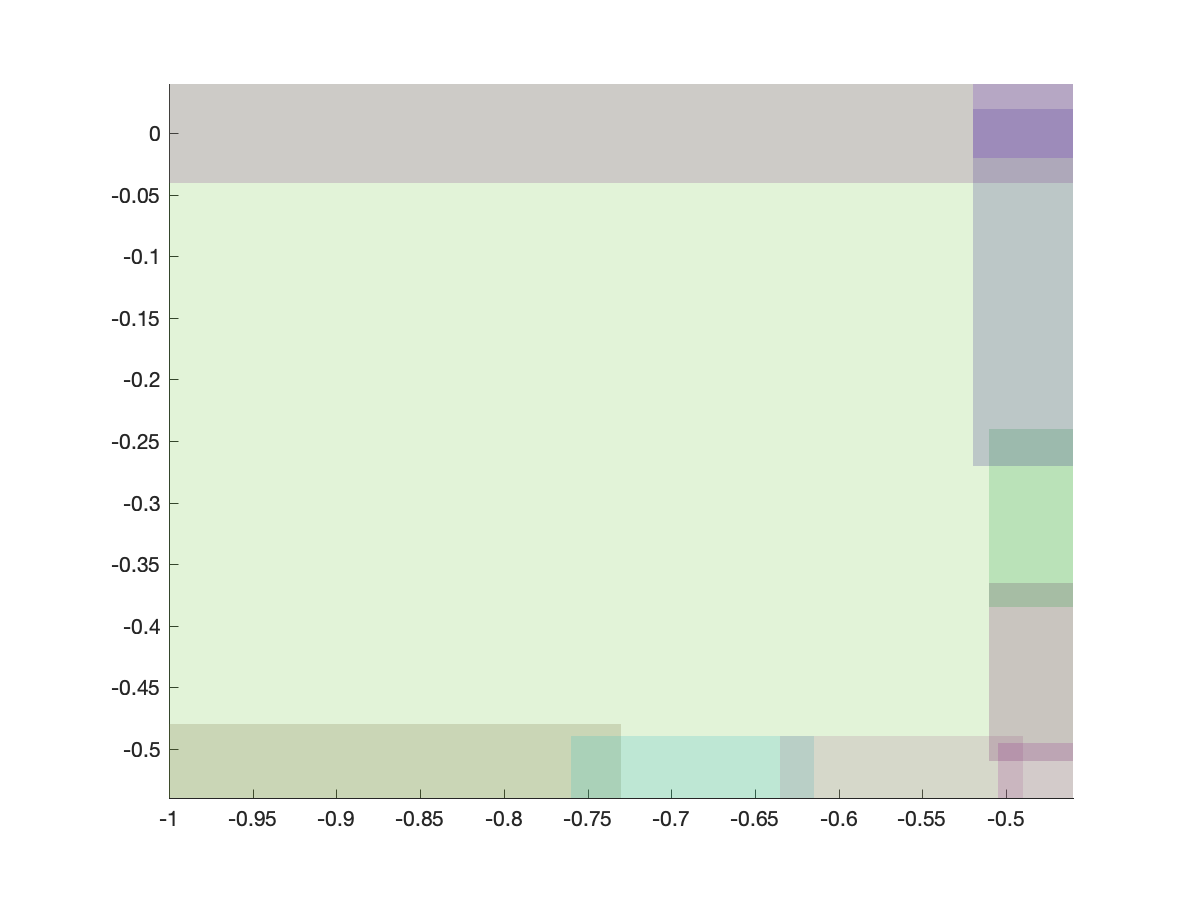
\includegraphics[scale = 0.5]{Chapter2/overlap.eps}
\caption{Plot of the subdomains formed from the partition of unity method for $\arctan(3(y^2+x))$ on a local patch with domain $[-1 , -0.46] \times [-0.54 , 0.04]$.}
\label{overlap_plot}
\end{figure}

Next we describe efficient algorithms using the tree representation of the global approximant to perform common numerical operations such as evaluation at points, basic binary arithmetic operations on functions, differentiation, and integration.

\subsection{Evaluation}

Note that (\ref{eq:pu-weight})--~(\ref{eq:pu-approx}) can be rearranged into
\begin{equation}
  s(\vect{x}) = \sum_{\nu\in \text{leaves}(\ct)} \frac{s_\nu(\vect{x}) \psi_\nu(\vect{x})}{\displaystyle \sum_{\mu\in \text{leaves}(\ct)} \psi_\mu(\vect{x})}
  = \frac{\displaystyle\sum_{\nu\in \text{leaves}(\ct)} s_\nu(\vect{x}) \psi_\nu(\vect{x})}{\displaystyle \sum_{\mu\in \text{leaves}(\ct)} \psi_\mu(\vect{x})}.
  \label{eq:pu-alt}
\end{equation}
This formula suggests a recursive approach to evaluating the numerator and denominator, presented in Algorithm~\ref{alg:numden}. Using it, only leaves containing $\vect{x}$ and their ancestors are ever visited. A similar approach was described in~\cite{tobor2006reconstructing}.

\begin{algorithm}
\caption{[$S$,$P$]=numden($\nu$,$\vect{x}$)}
\label{alg:numden}
\begin{algorithmic}
\STATE $S=0$, $P=0$
\IF{$\nu$ is a leaf}
\STATE $S=\psi_\nu(\vect{x})$
\STATE $P = S \cdot \textsf{interpolant}(\nu)(\vect{x})$
\ELSE
\FOR{$k=0,1$}
\IF{$\vect{x} \in \text{\textsf{domain}(\child{k}}(\nu))$}
\STATE $[S_k,P_k]$ = numden(\child{k}($\nu$),$\vect{x}$) 
\STATE $S = S + S_k$
\STATE $P = P + P_k$
\ENDIF
\ENDFOR
\ENDIF
\end{algorithmic}
\end{algorithm}

Algorithm~\ref{alg:numden} can easily be vectorized to evaluate $s(\vect{x})$ at multiple points, by recursively calling each leaf with all values of $\vect{x}$ that lie within its domain. In the particular case when the evaluation is to be done at all points in a Cartesian grid, it is worth noting that the leaf-level interpolant in~(\ref{eq:full-interp}) can be evaluated by a process that yields significant speedup over a naive approach. As a notationally streamlined example, say that the desired values of $\vect{x}$ are $(\xi_{j_1},\ldots,\xi_{j_d})$, where each $j_k$ is drawn from $\{1,\ldots,M\}$, and that the array of polynomial coefficients is of full size $O(N^d)$. Express~(\ref{eq:full-interp}) as
\begin{multline}
  \label{eq:grid-eval}
  \sum_{i_1=0}^{\nmax-1} \cdots \sum_{i_d=0}^{\nmax-1}  C_{i_1,\ldots,i_d} T_{i_1}(\xi_{j_1})\cdots T_{i_d}(\xi_{j_d})
  \\ = \sum_{i_1=0}^{\nmax-1} T_{i_1}(\xi_{j_1}) \sum_{i_2=0}^{\nmax-1} T_{i_2}(\xi_{j_2}) \cdots \sum_{i_d=0}^{\nmax-1}  C_{i_1,\ldots,i_d} T_{i_d}(\xi_{j_d}).
\end{multline}
The innermost sum yields $N^{d-1}M$ unique values, each taking $\bigo(N)$ time to compute. At the next level there are $N^{d-2}M^2$ values, and so on, finally leading to the computation of all $M^d$ interpolant values. This takes $\bigo(MN(M+N)^{d-1})$ operations, as opposed to $\bigo(M^dN^d)$ when done naively. 



\subsection{Binary arithmetic operations}

Suppose we have two approximations ${s}_1(\vect{x})$, ${s}_2(\vect{x})$, represented by trees $\ct_1$ and $\ct_2$ respectively, and we want to construct a tree approximation for ${s}_1 \circ {s}_2$, where $\circ$ is one of the operators $+$, $-$, $\times$, or $\div$. If $\ct_1$ and $\ct_2$ have identical tree structures, then it is straightforward to operate leafwise on the polynomial approximations. In the cases of multiplication and division, the resulting tree may have to be refined further using Algorithm~\ref{alg:split}, since these operations typically result in polynomials of degree greater than the operands. 

If the trees $\ct_1$ and $\ct_2$ are not structurally identical, we are free to use Algorithm~\ref{alg:split} to construct an approximation by sampling values of ${s}_1 \circ {s}_2$. However, the tree of ${s}_1 \circ {s}_2$ likely shares refinement structure with both $\ct_1$ and $\ct_2$. For example, Figure~\ref{zone_tan} shows the refined zones of the trees for $\arctan(100(x^2+y))$, $\arctan(100(x+y^2))$, and their sum. Thus in practice we merge the trees $\ct_1$ and $\ct_2$ using Algorithm~\ref{alg:merge}, presented in Appendix~\ref{sec:merge}. The merged tree, whose leaves contain sampled values of the result, may then be refined further if chopping tests then reveal that the result is not fully resolved. 

\begin{figure}
\centering
\subfloat[Zone plot of $f_1(x,y)$]{
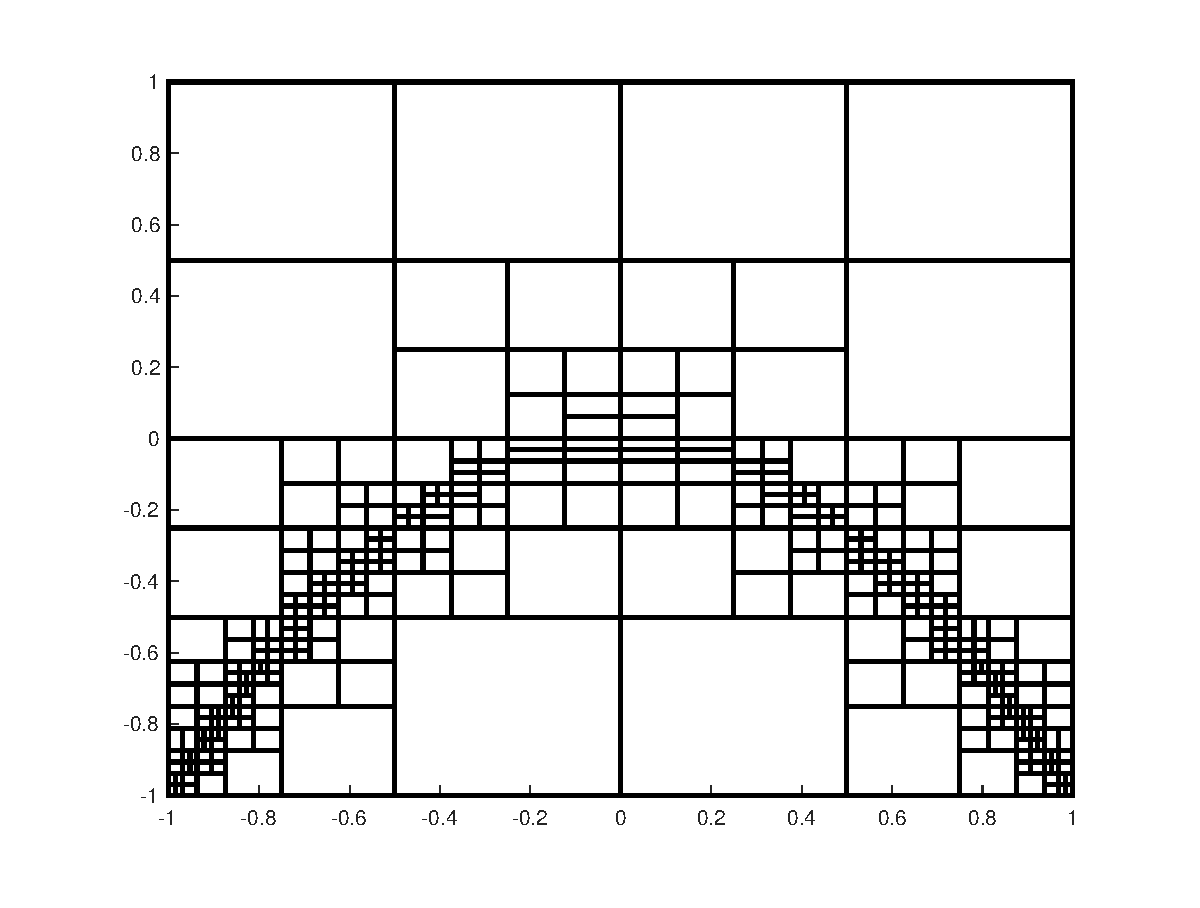
\includegraphics[scale = 0.3]{Chapter2/tan_100_1.eps}
   \label{zone_tan_a}
 }
\subfloat[Zone plot of $f_2(x,y)$]{
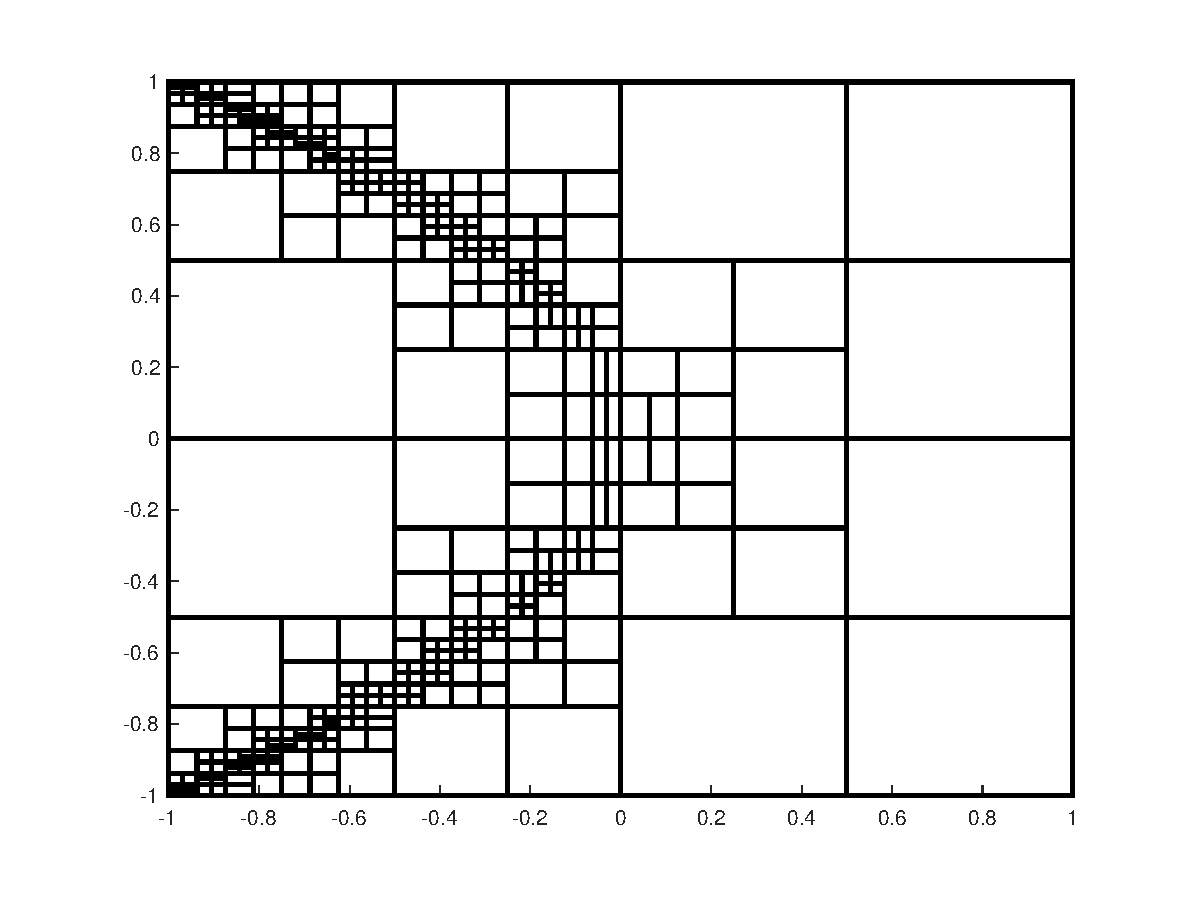
\includegraphics[scale = 0.3]{Chapter2/tan_100_2.eps}
   \label{zone_tan_b}
 }
 
 \subfloat[Zone plot of $f_1(x,y)+f_2(x,y)$]{
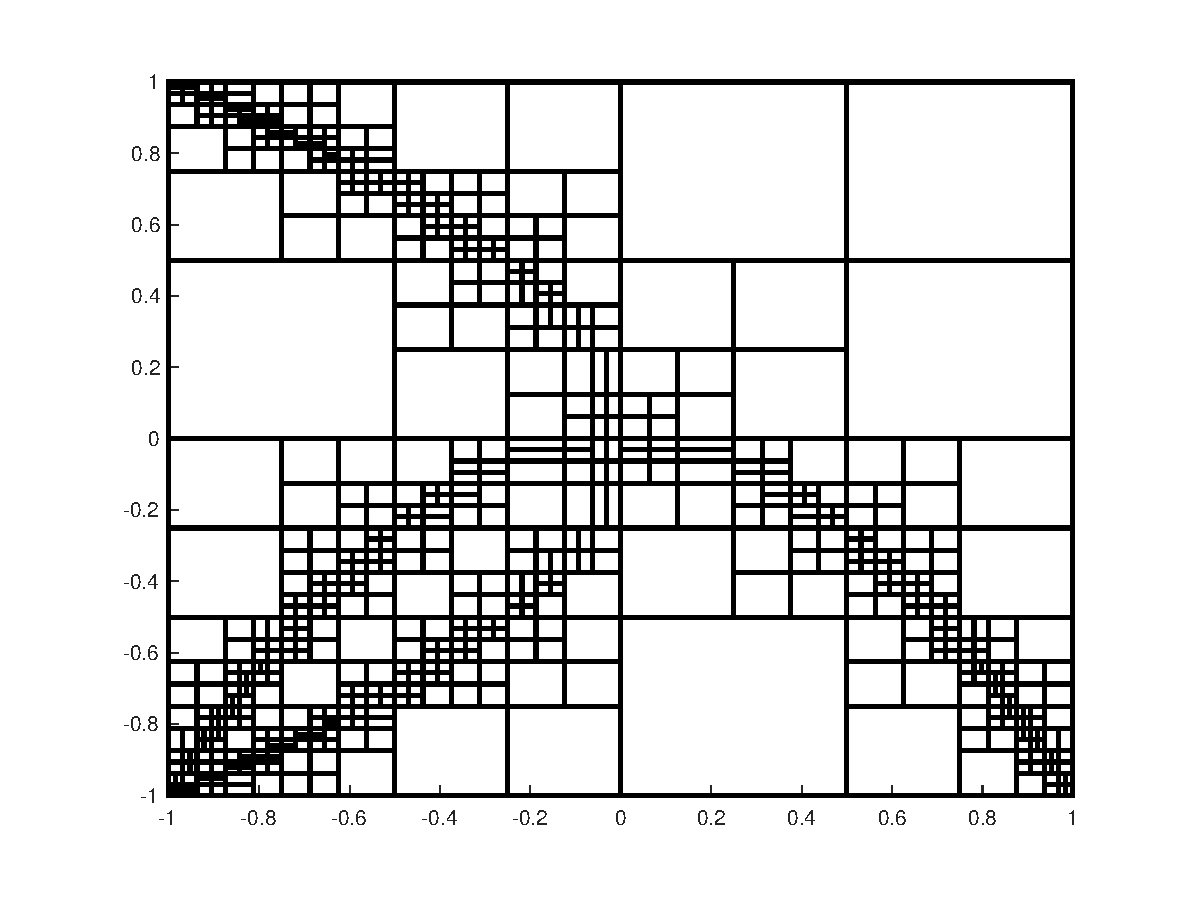
\includegraphics[scale = 0.3]{Chapter2/tan_100_3.eps}
   \label{zone_tan_c}
 }
 \caption{Zone plots for $f_1(x,y)$,$f_2(x,y)$ and $f_1(x,y)+f_2(x,y)$.}
\label{zone_tan}
\end{figure}
 




\subsection{Differentiation}

Differentiation of the global approximant~(\ref{eq:pu-approx}) results in two groups of terms:
\begin{equation*}
  \pp{}{x_j} s(\vect{x})=\sum_{\nu\in \text{leaves}(\ct)} w_\nu(\vect{x}) \pp{}{x_j} s_\nu(\vect{x})+\sum_{\nu\in \text{leaves}(\ct)} s_\nu(\vect{x}) \pp{}{x_j} w_\nu(\vect{x}).
%  \label{eq:pu-deriv}	
\end{equation*}
The first sum is a partition of unity approximation of leafwise differentiated interpolants. That is, we simply apply standard spectral differentiation to the data stored in the leaves of $\ct$. Although it may seem surprising at first, we can define the desired derivative approximation solely in terms of this first sum, and neglect the second with little penalty.

\begin{thm}
  Define
  \begin{equation}
    \label{eq:pu-deriv}
    s^{(j)}(\vect{x})=\sum_{\nu\in \text{leaves}(\ct)} w_\nu(\vect{x}) \pp{}{x_j} s_\nu(\vect{x}).
  \end{equation}
  Then for all $\vect{x}\in\Omega$,
  \begin{equation}
    \label{eq:pu-deriv-error}
    \left|s^{(j)}(\vect{x})-\pp{f}{x_j}(\vect{x})\right| \le \sum_{\vect{x} \in \prop{domain}{\nu}} w_\nu(\vect{x}) \left| \pp{s_\nu}{x_j}(\vect{x}) - \pp{f}{x_j} (\vect{x})\right|. %\le \sum_{\vect{x} \in \prop{domain}{\nu}} \left| \pp{s_\nu}{x_j}(\vect{x}) - \pp{f}{x_j} (\vect{x})\right|.
  \end{equation}
\end{thm}
\begin{proof}
  By the partition of unity property,
  \[
    s^{(j)}(\vect{x})-\pp{f}{x_j}(\vect{x}) = \sum_{\nu\in \text{leaves}(\ct)} w_\nu(\vect{x}) \left[\pp{}{x_j} s_\nu(\vect{x}) - \pp{f}{x_j}(\vect{x})\right].
  \]
  The result follows because $w_\nu(\vect{x})=0$ if $\vect{x}\notin \prop{domain}{\nu}$.%, and $|w_\nu(\vect{x})|\le 1$ for all $\vect(x)$. 
\end{proof}

Hence if $\vect{x}$ is not in an overlap region, the error in the global derivative approximation $s^{(j)}$ is the same as for the local approximant. Otherwise, it is bounded---pessimistically, since the weights are positive and sum to unity pointwise---by the sum of errors in all the contributing approximants. Since no point can be in more than $2^d$ subdomains (and then only near a meeting of hyperrectangle corners), we feel this error is acceptable in two and three dimensions.  

% For the second sum, note that the weight function derivatives are nonzero only at values of $\vect{x}$ that lie in the domains of more than one leaf; elsewhere the weight functions are identically one or zero. If the values of all the leafwise interpolants agree perfectly at such $\vect{x}$, then
% \begin{equation}
%   \label{eq:pu-weight-deriv}
%   \sum_{\nu\in \text{leaves}(\ct)} s_\nu(\vect{x}) \pp{}{x_j} w_\nu(\vect{x})
%   = s_\nu(\vect{x}) \pp{}{x_j}  \sum_{\nu\in \text{leaves}(\ct)} w_\nu(\vect{x}) = 0,
% \end{equation}
% since the weights are a partition of unity. Thus this term essentially contributes an amount on the order of the local interpolation accuracy times the gradients of the weights. These gradients are inversely proportional to the overlap widths, which are themselves proportional to the zone widths (see~(\ref{eq:overlap})). At most, then, they contribute an amount that is $\bigo(2^m)$ larger than the original local error on a leaf that is at depth $m$ in the tree. As a practical issue, we are unlikely to be able to cope anyway with a tree of depth great enough to incur a factor as large as two full orders of magnitude---which we would need only to resolve features at a scale much less than 1\% of the original domain width. Hence we feel justified ignoring this contribution. 


\subsection{Integration}

The simplest and seemingly most efficient approach to integrating over the domain is to do so piecewise over the nonoverlapping zones,
\begin{equation}
  \label{eq:integration}
  \int_{\Omega} f(\vect{x}) d\vect{x} = \sum_{\nu\in \text{leaves}(\ct)} \int_{\text{\textsf{zone}($\nu$)}} f(\vect{x}) d\vect{x}.
\end{equation}
Since the leaf interpolants are defined natively over the overlapping domains, they must be resampled at Chebyshev grids on the zones, after which Clenshaw-Curtis quadrature is applied.

\section{Numerical experiments}
\label{sec:numerical_experiments}

All the following experiments were performed on a computer with a 2.6 GHz Intel Core i5 processor in version 2017a of MATLAB. Our code, which uses a serial object-oriented recursive implementation of the algorithms, is available for download.\footnote{\url{https://github.com/kevinwaiton/PUchebfun}} Comparisons to Chebfun2 and Chebfun3 were done using Chebfun version 5.5.0. We also tried to use the Sparse Grid Interpolation Toolbox~\cite{Klimke2005}, but on all the examples we were unable to get it close to our desired error tolerances within its hard-coded limits on sparse grid depth. 

\subsection{2D experiments}

We first test the 2D functions $\log(1+(x^2+y^4)/10^{-5})$, $\arctan((x+y^2)/10^{-2})$, $\frac{10^{-4}}{(10^{-4}+x^2)(10^{-4}+y^2)}$, Franke's function \cite{franke1979critical}, the smooth functions from the Genz family test package \cite{genz1987package}, and the ``peg'' examples from~\cite{trefethen2017cubature}. For each function we record the time of construction, the time to evaluate on a $200\times 200$ grid, and the max observed error on this grid. Table~\ref{tab:timing2D} shows the results for the new method. For the low-rank test cases, the methods are comparable, with neither showing a consistent advantage; most importantly, both methods are fast enough for interactive computing. In the tests of higher-rank functions, the tree-based method exhibits a clear, sometimes dramatic, advantage in construction time. Moreover, the tree method remains fast enough for interactive computing even as the total number of nodes exceeds 1.6 million.  We present plots of the functions and adaptively generated subdomains for the first three test functions in Figures~\ref{TANFUN1}-\ref{rungeFUN1}.

\begin{table}[p]

  \begin{tabular}{c|c|c|c|c|c}
    \multirow{2}{*}{Function} & \multirow{2}{*}{Alg.} & \multirow{2}{*}{Error} & Build & Eval & Points /  \\
                            & &  & time & time & Rank  \\ \hline
    \multirow{2}{*}{$\log(1+\frac{x_1^2+x_2^4}{10^{-5}})$} &  T & 1.16$\times 10^{-15}$ &	0.525 &	0.1235 & 69800 \Tstrut  \\
                              & C & 1.14$\times 10^{-6}$ & 2.30 & 0.10 & 30 \\ \hline
    \multirow{2}{*}{$\arctan(\frac{x_1+x_2^2}{10^{-2}})$} & T & 1.83$\times 10^{-14}$ &	2.241 & 0.3590	& 917515 \Tstrut\\
                              & C & 7.09$\times 10^{-12}$ & 150 & 5.0 & 816 \\ \hline
    \multirow{2}{*}{$\frac{10^{-4}}{(10^{-4}+x_1^2)(10^{-4}+x_2^2)}$} & T & 1.86$\times 10^{-15}$ & 0.606 & 0.0728 & 	117056 \Tstrut\\
                              & C & 5.44$\times 10^{-15}$ & 0.049 & 0.0037 & 1 \\ \hline
    \multirow{2}{*}{franke} & T & 1.33$\times 10{-15}$ & 	0.061 &	0.0069 &	9270 \Tstrut\\
                              & C & 1.33$\times 10^{-15}$ & 0.020 & 0.0024 & 4 \\ \hline
    \multirow{2}{*}{$\cos(u_1\pi + \sum_{i=1}^2 a_i x_i)$} & T & 23.00$\times 10^{-15}$ &	0.007 &	0.0012 & 	972 \Tstrut\\
                              & C & 4.47$\times 10^{-14}$ & 0.016 & 0.0020 & 2 \\ \hline
    \multirow{2}{*}{$\prod_{i=1}^2 (a_i^{-2}+(x_i-u_i)^2)^{-1}$} & T & 2.01$\times 10^{-15}$ &	0.063 &	0.0099 & 21232 \Tstrut\\
                              & C & 1.59$\times 10^{-12}$ & 0.020 & 0.0022 & 1 \\ \hline
    \multirow{2}{*}{$(1+\sum_{i=1}^2 a_i x_i)^{-3}$} & T & 3.33$\times 10^{-16}$ &	0.006 &	0.0004 &	 25 \Tstrut\\
                              & C & 2.27$\times 10^{-12}$ & 0.012 & 0.0021 & 4 \\ \hline
    \multirow{2}{*}{$\exp(-\sum_{i=1}^2 a_i^2 (x_i-u_i)^2)$} & T & 7.77$\times 10{-16}$ & 0.005 &	0.0012 & 	1862 \Tstrut\\
                              & C & 4.44$\times 10^{-16}$ & 0.015 & 0.0022 & 1 \\  \hline
    \multirow{2}{*}{square peg} & T & 2.22$\times 10^{-15}$ & 0.126 &	0.0264 & 111188 \Tstrut\\
                              & C & 1.22 $\times 10^{-15}$ &	0.023 &	0.0012 & 	1 \\ \hline
    \multirow{2}{*}{tilted peg} & T & 2.00$\times 10^{-15}$ &	0.214 &	0.0375 & 117544 \Tstrut\\
                              & C & 7.68$\times 10^{-14}$ & 0.265 & 	0.0181 & 100
                              
  \end{tabular}
  \caption{Observed error and wall-clock times for the tree-based (T) and Chebfun2 (C) algorithms with target tolerance $10^{-16}$ and $\nmax=129$. Build time is for constructing the approximation object, and eval time for evaluating an approximant on a 200x200 uniform grid (all times in seconds). Also shown: for the tree-based method, the total number of stored sampled function values, and for Chebfun2, the numerically determined rank of the function. Here $u=[0.75,0.25]$ and $a=[5,10]$.}
  \label{tab:timing2D}
% \begin{tabular}{r|c|c|c|c|c|c}
% Function & method & error & construct time & eval time & int time & points \\[5pt] \hline
%   \multirow{2}{*}{$\log(1+\frac{x_1^2+x_2^4}{10^{-5}})$} &  tree-based & 1.05$\times 10^{-13}$ & 0.6403 & 0.063 & 0.081 & 110496 \\
%   & Chebfun2 & 1.14$\times 10^{-6}$ & 2.2997 & 0.1045 & 0.004 & 30 \\ \hline
%   \multirow{2}{*}{$\arctan(\frac{x_1+x_2^2}{10^{-2}})$} & tree-based & 2.15$\times 10^{-12}$ & 2.9690 & 0.3138 & 0.528 & 1553816 \\
%   & Chebfun2 & 7.09$\times 10^{-12}$ & 150.2228 & 4.979 & 0.017 & 816 \\ \hline
%   \multirow{2}{*}{$\frac{10^{-4}}{(10^{-4}+x_1^2)(10^{-4}+x_2^2)}$} & tree-based & 1.01$\times 10^{-11}$ & 0.7298 & 0.1087 & 0.093 & 145280 \\
%   & Chebfun2 & 5.44$\times 10^{-15}$ & 0.0493 & 0.0037 & 0.001 & 1 \\ \hline
%   \multirow{2}{*}{franke} & tree-based & 4.22$\times 10^{-15}$ & 0.0116 & 0.0045 & 0.007 & 16641 \\
%   & Chebfun2 & 1.33$\times 10^{-15}$ & 0.0198 & 0.0024 & 0.001 & 4 \\ \hline
%   \multirow{2}{*}{$\cos(u_1\pi + \sum_{i=1}^2 a_i x_i)$} & tree-based & 2.65$\times 10^{-14}$ & 0.0127 & 0.0025 & 0.002 & 1089 \\
%   & Chebfun2 & 4.47$\times 10^{-14}$ & 0.0155 & 0.002 & 0.001 & 2 \\ \hline
%   \multirow{2}{*}{$\prod_{i=1}^2 (a_i^{-2}+(x_i-u_i)^2)^{-1}$} & tree-based & 5.00$\times 10^{-12}$ & 0.0555 & 0.016 & 0.011 & 29283 \\
%   & Chebfun2 & 1.59$\times 10^{-12}$ & 0.0203 & 0.0022 & 0.001 & 1 \\ \hline
%   \multirow{2}{*}{$(1+\sum_{i=1}^2 a_i x_i)^{-3}$} & tree-based & 2.27$\times 10^{-12}$ & 0.0119 & 8.97$\times 10^{-4}$ & 0.001 & 25 \\
%   & Chebfun2 & 2.27$\times 10^{-12}$ & 0.0117 & 0.0021 & 0.001 & 4 \\ \hline
%   \multirow{2}{*}{$\exp(-\sum_{i=1}^2 a_i^2 (x_i-u_i)^2)$} & tree-based & 1.65$\times 10^{-14}$ & 0.0130 & 0.0026 & 0.002 & 2145 \\
%   & Chebfun2 & 4.44$\times 10^{-16}$ & 0.0149 & 0.0022 & 0.001 & 1 
% \end{tabular}
% \caption{Observed error and wall-clock time for the tree method to construct tree-based and Chebfun2 approximations with target tolerance $10^{-12}$ and $\nmax=129$, and to evaluate it on a 200x200 uniform grid. Also shown is the total number of sampled function values stored over all the leaves of the tree. Here $u=[0.75,0.25]$, and $a=[5,10]$.}
% \label{putable}
\end{table}

%\begin{table}
%\begin{tabular}{cccccc}
%& Algorithm & relative error & build time & eval time & rank \\
%log(1+(x^2+y^4)/1e-5) & T & 1.16E-15 & 0.525 & 0.1235 & 69800 \\
%& C & 1.68E-06 & 3.201 & 0.0885 & 27 \\
%arctan((x+y^2)/1e-1) & T & 1.83E-14 & 2.241 & 0.3590 & 917515 \\
%& C & 2.55E-12 & 177.081 & 1.3498 & 816 \\
%1e-4/((1e-4+x^2)(1e-4+y^2)) & T & 1.86E-15 & 0.606 & 0.0728 & 117056 \\
%& C & 9.28E-15 & 0.068 & 0.0038 & 1 \\
%franke & T & 1.33E-15 & 0.061 & 0.0069 & 9270 \\
%& C & 6.65E-16 & 0.037 & 0.0023 & 4 \\
%Gens f1 & T & 3.00E-15 & 0.007 & 0.0012 & 972 \\
%& C & 3.17E-15 & 0.022 & 0.0016 & 2 \\
%Gens f2 & T & 2.01E-15 & 0.063 & 0.0099 & 21232 \\
%& C & 7.29E-16 & 0.026 & 0.0014 & 1 \\
%Gens f3 & T & 3.33E-16 & 0.006 & 0.0004 & 25 \\
%& C & 4.44E-16 & 0.014 & 0.0012 & 4 \\
%Gens f4 & T & 7.77E-16 & 0.005 & 0.0012 & 1862 \\
%& C & 4.44E-16 & 0.019 & 0.0021 & 1 \\
%square peg & T & 2.22E-15 & 0.126 & 0.0264 & 111188 \\
%& C & 1.22E-15 & 0.023 & 0.0012 & 1 \\
%tilted peg & T & 2.00E-15 & 0.214 & 0.0375 & 117544 \\
%& C & 7.68E-14 & 0.265 & 0.0181 & 100 \\
%\end{tabular}
%  \caption{Observed error and wall-clock times for the tree-based (T) and Chebfun2 (C) algorithms with target tolerance $10^{-12}$ and $\nmax=129$. Build time is for constructing the approximation object, and eval time for evaluating an approximant on a 200x200 uniform grid (all times in seconds). Also shown: for the tree-based method, the total number of stored sampled function values, and for Chebfun2, the numerically determined rank of the function. Here $u=[0.75,0.25]$ and $a=[5,10]$.}
%\end{table}


\begin{figure}
  \centering
  \subfloat[$\arctan \lp (x+y^2)/0.01 \rp$]{
    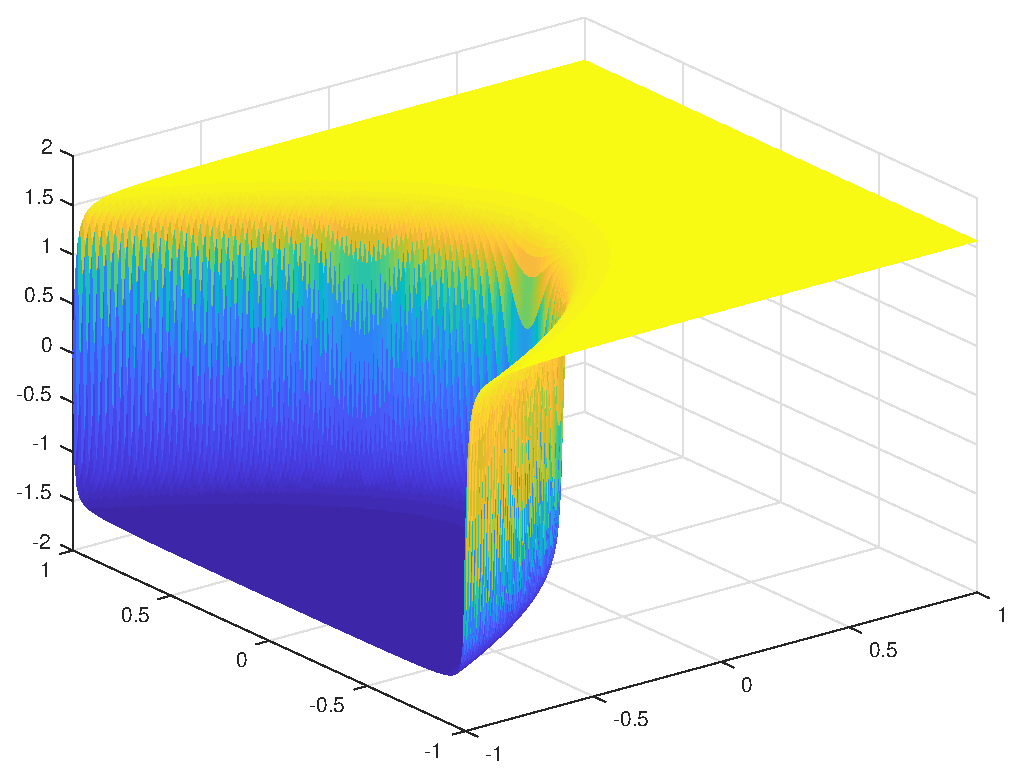
\includegraphics[scale = 0.34]{Chapter2/tan2Dplot}
    \label{tanfunplot}
  }
  \subfloat[Overlapping subdomains]{
    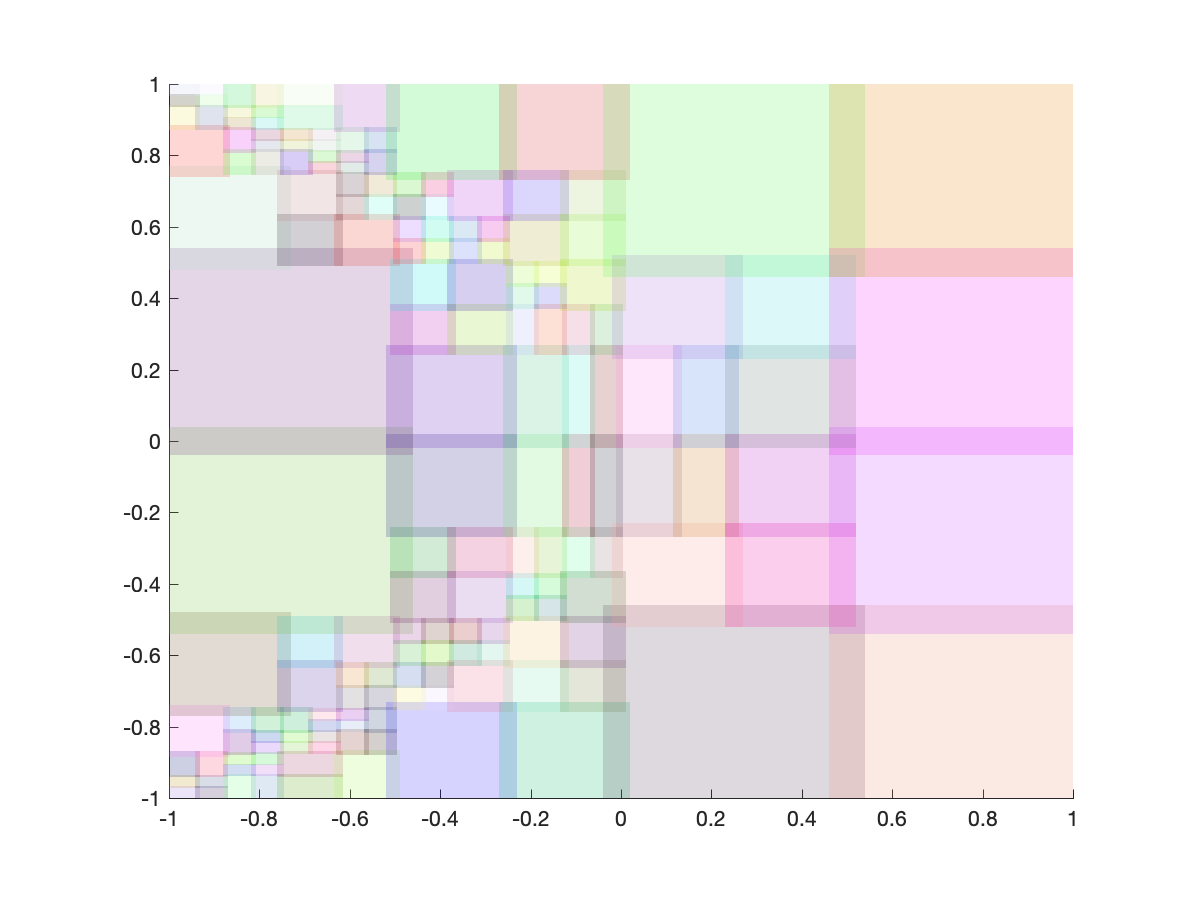
\includegraphics[scale = 0.34]{Chapter2/tan2Dsubdomains}
    \label{tanfundomains}
  }
  \caption{Overlapping subdomains constructed by the adaptive tree method for a function with a nonlinear ``cliff.''}
  \label{TANFUN1}
\end{figure}

\begin{figure}
  \centering
  \subfloat[$\frac{10^{-4}}{(10^{-4}+x^2)(10^{-4}+y^2)}$]{
    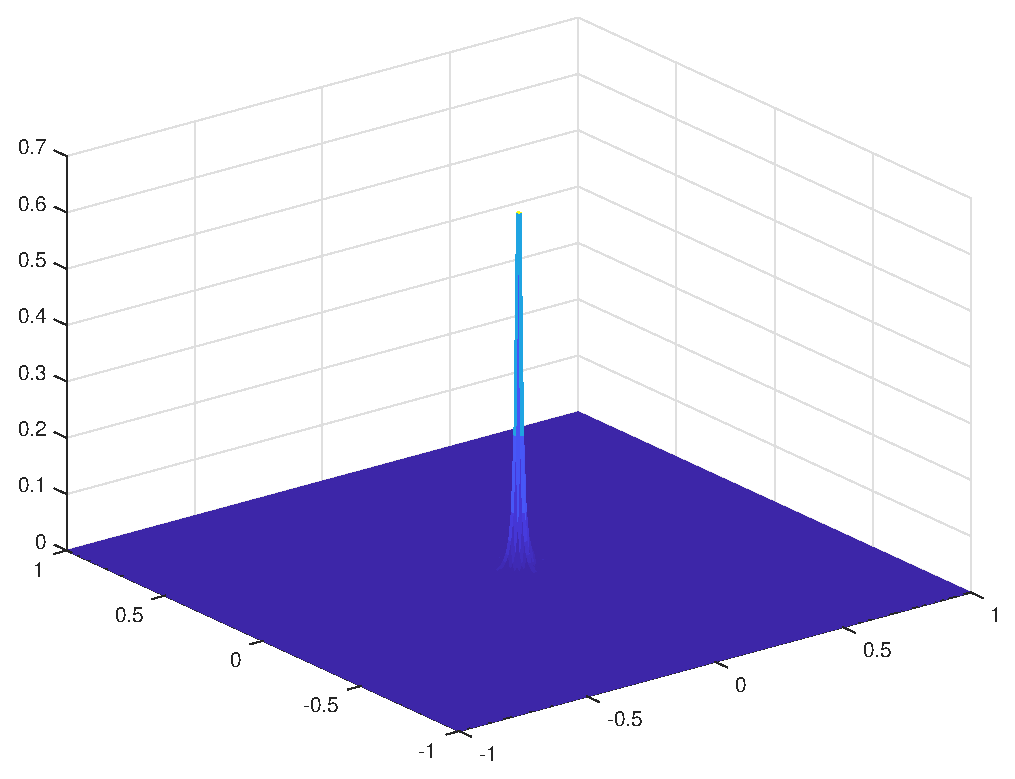
\includegraphics[scale = 0.34]{Chapter2/runge2Dplot}
    \label{rungefunplot}
  }
  \subfloat[Overlapping subdomains]{
    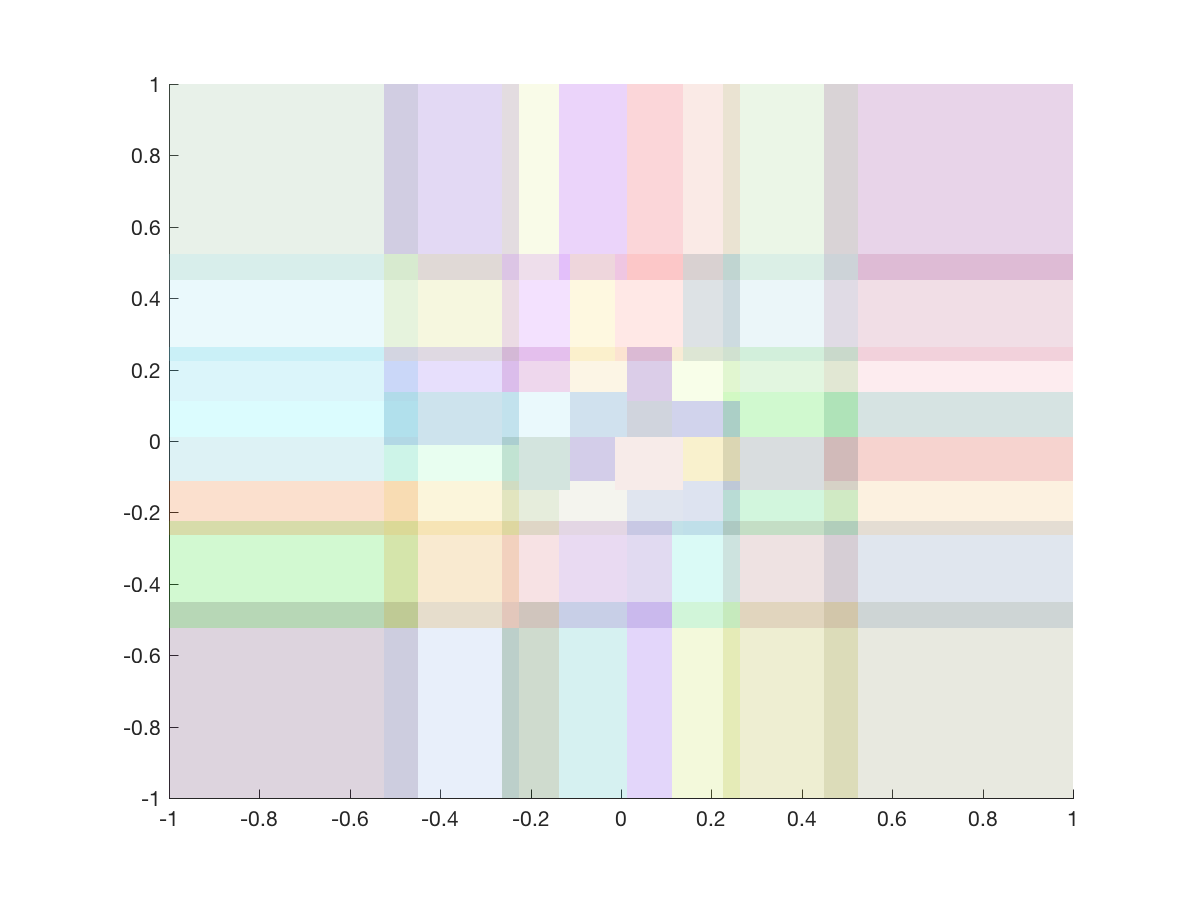
\includegraphics[scale = 0.34]{Chapter2/rungesubdomains}
    \label{rungefundomains}
  }
  \caption{Overlapping subdomains constructed by the adaptive tree method for a function with a sharp spike.}
  \label{rungeFUN1}
\end{figure}


One important aspect of low-rank approximation is that it is inherently nonisotropic. Consider the 2D ``plane wave bump'' 
\begin{equation}
f(x,y)=\arctan(250(\cos(t)x+\sin(t)y))
\label{rotate_func_2D}	
\end{equation}
whose normal makes an angle $t$ with the positive $x$-axis. We compare the construction times of our method to Chebfun2 for $t \in [0,\pi/4]$ in Figure~\ref{tan_rotate_2D}. We observe the execution time of Chebfun2 varying over nearly three orders of magnitude. While our method is also responsive to the angle of the wave, the variation in time is about half an order of magnitude, and our codes are faster in all but the rank-one case $t=0$ (for which both methods are fast). 


\begin{figure}
\centering
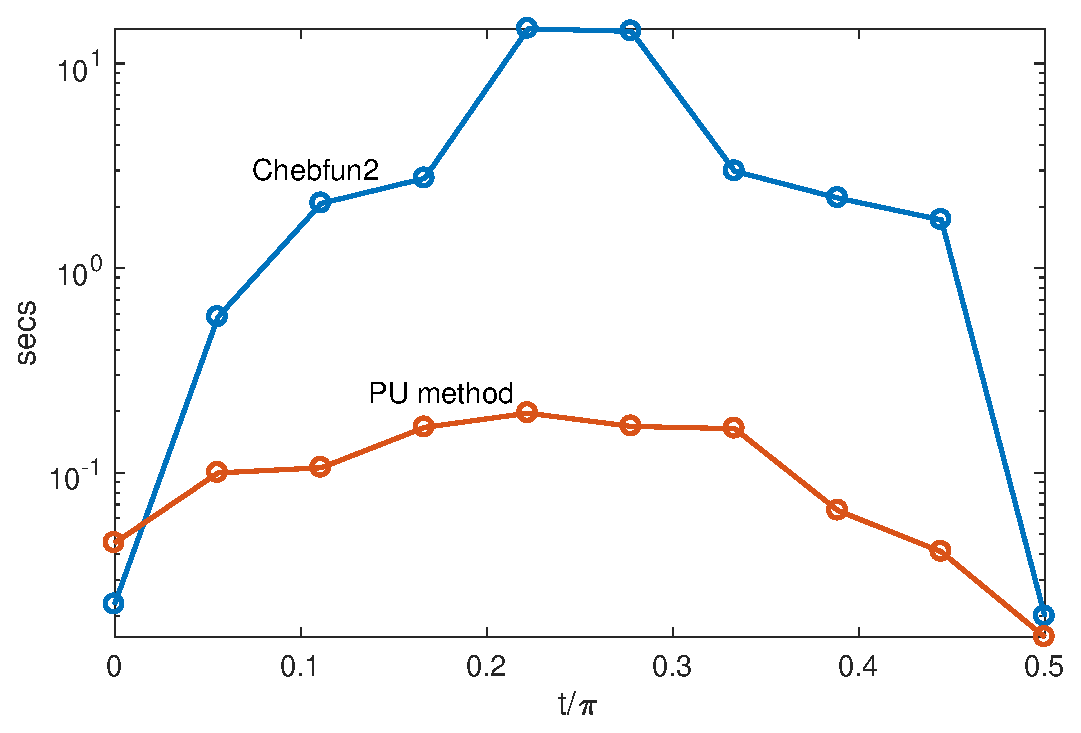
\includegraphics[scale = 0.5]{Chapter2/tan_rotate_2D}
\caption{Comparison of construction times for $\arctan(250(\cos(t)x+\sin(t)y))$ for $t \in [0,\pi/4]$.}
\label{tan_rotate_2D}
\end{figure}


Our next experiment is to add and multiply the rank-one function $\arctan(250x)$ to the plane wave in~(\ref{rotate_func_2D}). The construction time results are compared for $t \in [0,\pi/2]$ in Figure~\ref{TAN_ADD_MULT}. Here the dependence of Chebfun2 on the angle is less severe than in the simple construction, though it is still more pronounced than for our method. More importantly, the absolute numbers for addition in particular with Chebfun2 would probably be considered unacceptable for interactive computation, while our method takes one second at most. 

\begin{figure}
\centering
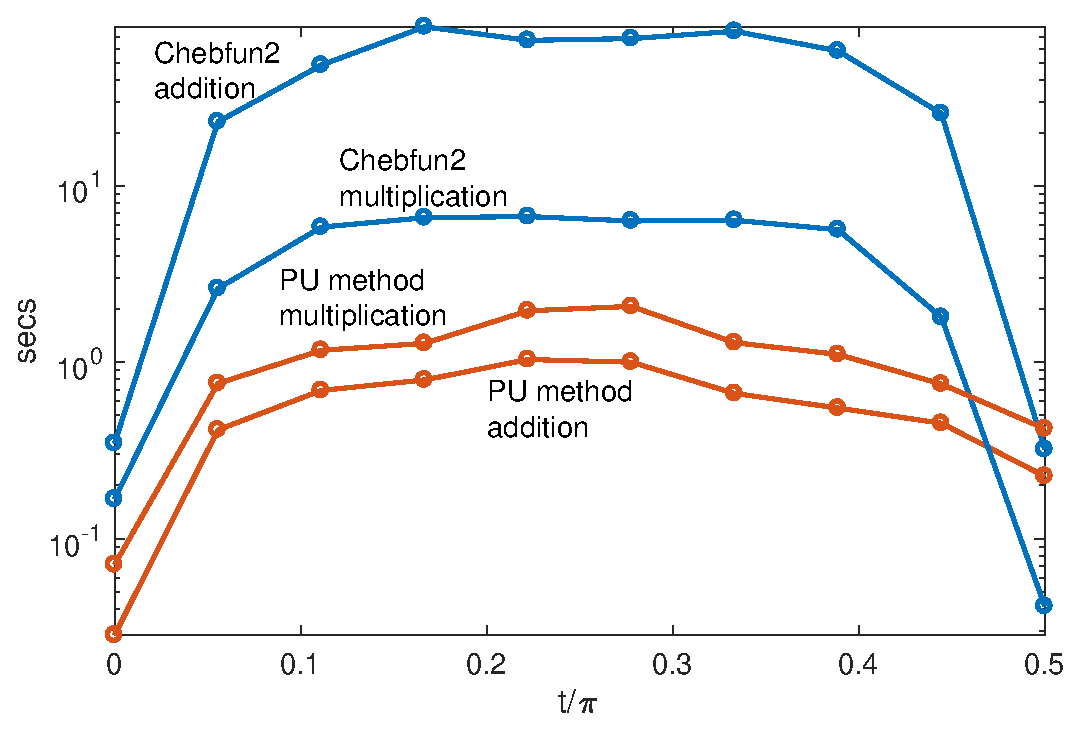
\includegraphics[scale = 0.5]{Chapter2/tan_rotate_add_mult_2D}
\caption{Comparison of execution times for multiplication and addition of $\arctan(250x)$ with $\arctan(250(\cos(t)x+\sin(t)y))$ for $t \in [0,\pi/4]$.}
\label{TAN_ADD_MULT}
\end{figure}



% \begin{figure}
% \centering
% \subfloat[Plot of $\log(1+(x^2+y^4)/10^{-5})$.]{
% 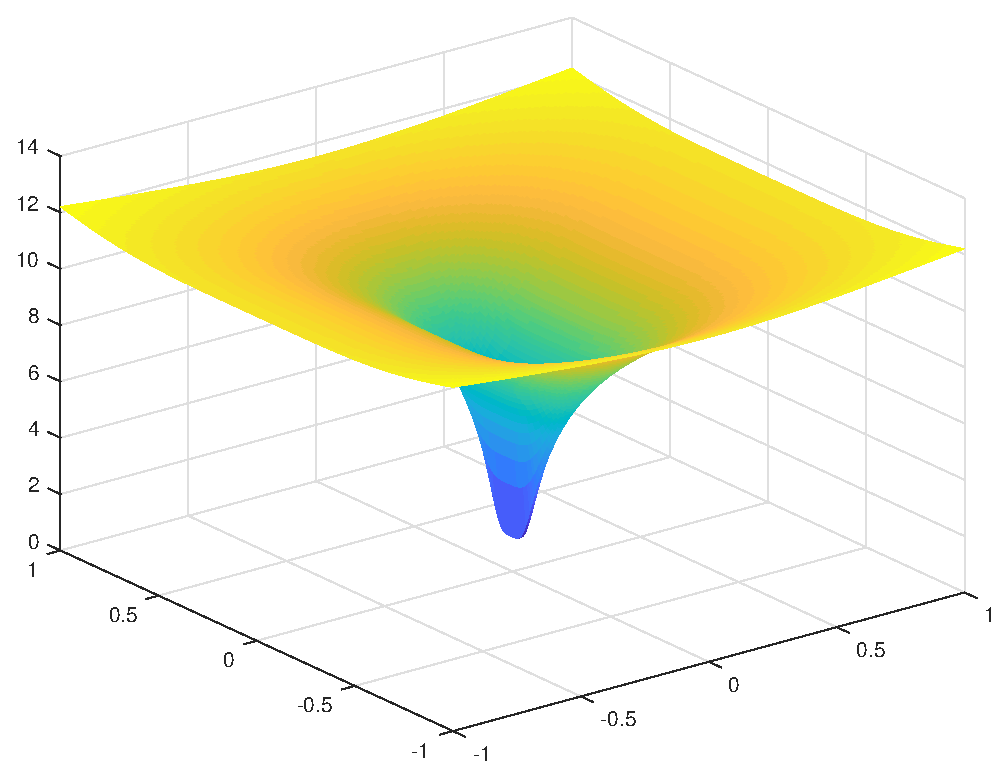
\includegraphics[scale = 0.34]{log2Dplot.eps}
%    \label{logfunplot}
%  }
% \subfloat[Plot of subdomains.]{
% 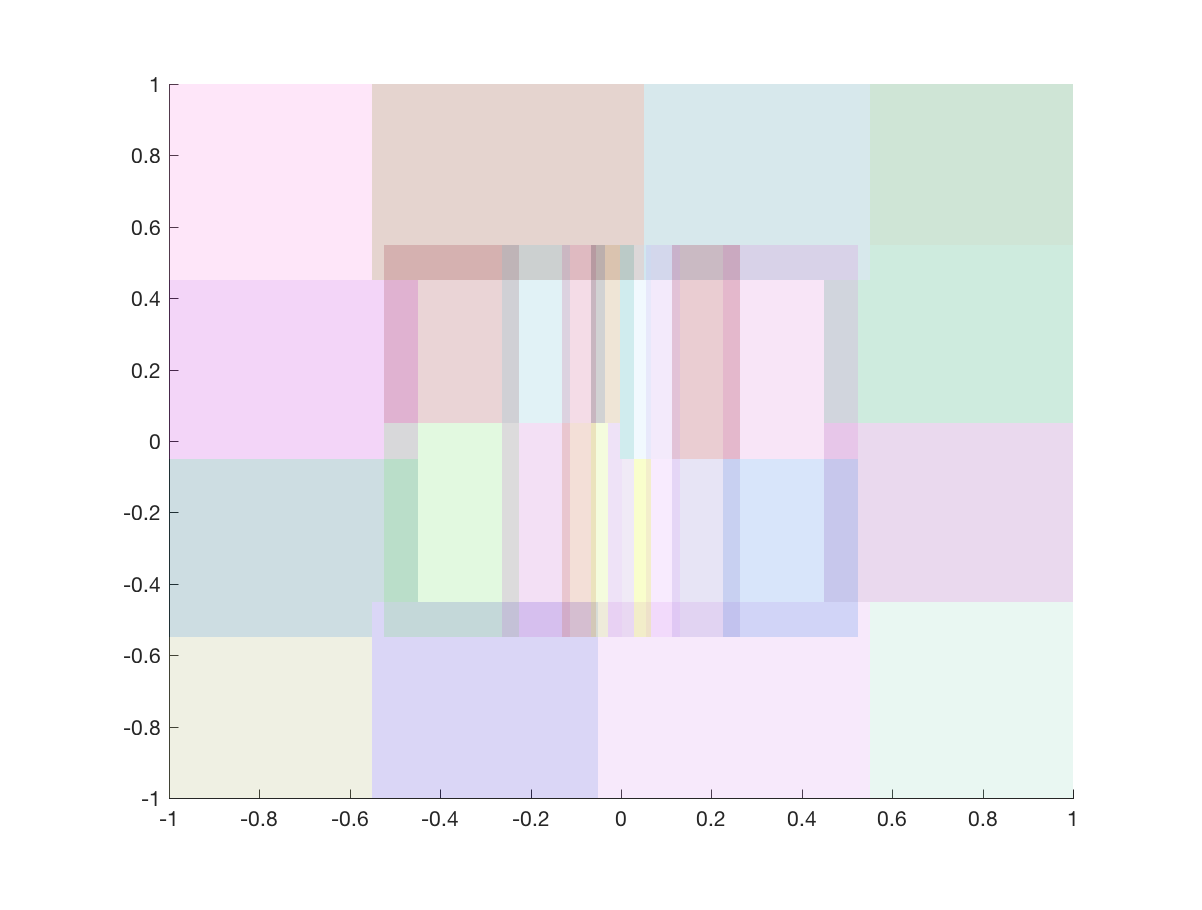
\includegraphics[scale = 0.34]{log2Dsubdomains.eps}
%    \label{logfundomains}
%  }
% \caption{Plot of $\log(1+(x^2+y^4)/10^{-5})$ and the subdomains formed from the partition of unity method.}
% \label{logFUN1}
% \end{figure}


\subsection{3D experiments}

We next test the 3D functions $1/(\cosh(5(x+y+z)))^2$, $\arctan(5(x+y)+z)$, and 3D versions of the smooth functions from the Genz family test package. Table~\ref{tab:timing3D} shows the construction time, the time taken to evaluate on a $200\times 200 \times 200$ grid, and the max error on this grid. We observe dramatic construction timing differences in every case: Chebfun3 outperforms the tree-based method for low-Tucker-rank functions, while for the two higher-rank cases, the tree-based method is the clear winner. Chebfun3 performance is more extreme in both senses, while the tree-based method is more consistent across these examples. Chebfun3 is also faster for evaluation overall, even in high-rank cases, though the evaluation times are typically far less than the construction times. 


\begin{table}[p]
  \begin{tabular}{c|c|c|c|c|c}
    \multirow{2}{*}{Function} & \multirow{2}{*}{Alg.} & \multirow{2}{*}{Error} & Build & Eval & Points /  \\
 & &  & time & time &Rank  \\ \hline
    \multirow{2}{*}{$\cos(u_1\pi + \sum_{i=1}^3 a_i x_i)$} & T & $3.16 \times 10^{-14}$ &	2.958 &	0.240 &	561495 \Tstrut\\
    & C & $2.19 \times 10^{-14}$ 	& 0.460 &	0.036 &	2 \\ \hline
    \multirow{2}{*}{$\prod_{i=1}^3 (a_i^{-2}+(x_i-u_i)^2)^{-1}$} & T & $2.37 \times 10^{-15}$ 	& 9.917 & 0.764 & 7751626 \Tstrut\\
    & C & $2.63 \times 10^{-15}$	 &  0.148 &	0.030 &	1 \\ \hline
    \multirow{2}{*}{$(1+\sum_{i=1}^3 a_i x_i)^{-4}$} & T & $5.58 10^{-16}$ & 0.351 &	0.020 &	216 \Tstrut\\
    & C & $8.93 \times 10^{-16}$ &	0.174 &	0.021 & 5\\ \hline
    \multirow{2}{*}{$\exp(-\sum_{i=1}^2 a_i^2 (x_i-u_i)^2)$} & T & $1.45\times 10^{-15}$ &	0.566 &	0.097 &	293305 \Tstrut  \\
    & C & $7.80 \times 10^{-16}$ &	0.066 &	0.018 & 1 \\ \hline
    \multirow{2}{*}{$1/(\cosh(5(x+y+z)))^2$} & T & $2.00\times 10^{-15}$	 & 4.337	 & 0.325 &	3450018 \Tstrut\\
    & C & $3.66 \times 10^{-13}$ 	& 74.446	 &0.050 &	93 \\ \hline
    \multirow{2}{*}{$\arctan(5(x+y)+z)$} & T & $1.95 \times 10^{-15}$ &	0.758	& 0.145	& 1132326 \Tstrut\\
    & C & $3.17\times 10^{-13}$	& 75.313	 & 0.033	& 110
  \end{tabular}
  \caption{Observed error and wall-clock times for the tree-based (T) and Chebfun3 (C) algorithms with target tolerance $10^{-16}$ and $\nmax=65$. Build time is for constructing the approximation object, and eval time for evaluating an approximant on a $200^3$ uniform grid (all times in seconds). Also shown: for the tree-based method, the total number of stored sampled function values, and for Chebfun3, the numerically determined rank of the function. Here $u=[0.75,0.25,-0.75]$ and $a=[25,25,25]$.} 
  \label{tab:timing3D}
\end{table}

% \begin{table}[p]
% \begin{tabular}{r|c|c|c|c}
% & error & construct time & eval time & rank \\[5pt] \hline
% $\cos(u_1\pi + \sum_{i=1}^2 a_i x_i)$ 
% $\prod_{i=1}^2 (a_i^{-2}+(x_i-u_i)^2)^{-1}$ [5pt]
% $(1+\sum_{i=1}^2 a_i x_i)^{-3}$ [5pt]
% $\exp(-\sum_{i=1}^2 a_i^2 (x_i-u_i)^2)$ [5pt]
% $1/(\cosh(5(x+y+z)))^2$ 
% $\arctan(5(x+y)+z)$ 
% \end{tabular}
% \caption{Observed error and wall-clock time for Chebfun3 using default settings to construct an approximation and evaluate it on a 200$^3$ uniform grid. Also shown is the computed rank of the function. Here $u=[0.75,0.25,-0.75]$ and $a=[25,25,25]$.}	
% \label{chb3table}
% \end{table}

% \begin{tabular}{r|c|c|c|c|c}
% & error & construct time & eval time & int time & points\\[5pt] \hline
% $\cos(u_1\pi + \sum_{i=1}^3 a_i x_i)$ & 22.71$\times 10^{-14}$ & 0.151 & 0.118 & 0.044 & 275000 \\ [5pt]
% $\prod_{i=1}^3 (a_i^{-2}+(x_i-u_i)^2)^{-1}$ & 1.52$\times 10^{-5}$ & 7.204 & 1.312 & 0.375 & 10400000 \\[2pt]
% $(1+\sum_{i=1}^3 a_i x_i)^{-3}$ & 4.66$\times 10^{-10}$ & 0.16555 & 0.033 & 0.001 & 125 \\[5pt]
% $\exp(-\sum_{i=1}^2 a_i^2 (x_i-u_i)^2)$ & 3.11$\times 10^{-15}$ & 0.0818 & 0.078 & 0.007 275000  \\[5pt]
% $1/(\cosh(5(x+y+z)))^2$ & 1.14$\times 10^{-14}$ & 0.706 & 0.545 & 0.043 & 2200000 \\
% $\arctan(5(x+y)+z)$ & 7.60$\times 10^{-13}$ & 0.7512 & 0.030 & 0.047 & 549153 \\
% \end{tabular}
% \caption{Observed error and wall-clock time for the tree method to construct a tree approximation with target tolerance $10^{-12}$ and $\nmax=65$, and to evaluate it on a 200$^3$ uniform grid. Also shown is the total number of sampled function values stored over all the leaves of the tree. Here $u=[0.75,0.25,-0.75]$ and $a=[25,25,25]$.}
% \label{putable3D}
% \end{table}

% \begin{table}[p]
% \begin{tabular}{r|c|c|c|c|c}
% & error & construct time & eval time & int time & rank \\[5pt] \hline
% $\cos(u_1\pi + \sum_{i=1}^2 a_i x_i)$ & 2.16$\times 10^{-14}$ & 0.061 & 0.150 & 0.006 & 2  \\[5pt]
% $\prod_{i=1}^2 (a_i^{-2}+(x_i-u_i)^2)^{-1}$ & 5.66$\times 10^{-7}$ & 0.057 & 0.137 & 0.002 & 1 \\[5pt]
% $(1+\sum_{i=1}^2 a_i x_i)^{-3}$ & 4.07$\times 10^{-10}$ & 0.038 & 0.143 & 0.001 & 4 \\[5pt]
% $\exp(-\sum_{i=1}^2 a_i^2 (x_i-u_i)^2)$ & 7.77$\times 10^{-16}$ & 0.047 & 0.144 & 0.001 & 1 \\[5pt]
% $1/(\cosh(5(x+y+z)))^2$ & 3.69$\times 10^{-13}$ & 80.666 & 0.398 & 0.002 & 93 \\
% $\arctan(5(x+y)+z)$ & 4.69$\times 10^{-13}$ & 89.957 & 0.104 & 0.001 & 110 \\
% \end{tabular}
% \caption{Observed error and wall-clock time for Chebfun3 using default settings to construct an approximation and evaluate it on a 200$^3$ uniform grid. Also shown is the computed rank of the function. Here $u=[0.75,0.25,-0.75]$ and $a=[25,25,25]$.}	
% \label{chb3table}
% \end{table}

We repeat our experiment testing the importance of axes alignment using the function
\begin{equation}
\arctan(5(\sin(p)\cos(t)x+\sin(p)\sin(t)y+\cos(p)z))
\end{equation}
for $p,t \in [0,\pi/4]$. Timing results can be seen in Figure~\ref{fig:tan3D}. As in 2D, the Chebfun low-rank technique shows wide variation depending on the angles, and a large region of long times. The tree-based method is much less sensitive and faster (by as much as two orders of magnitude) except for the purely axes-aligned cases. 

\begin{figure}
  \centering
  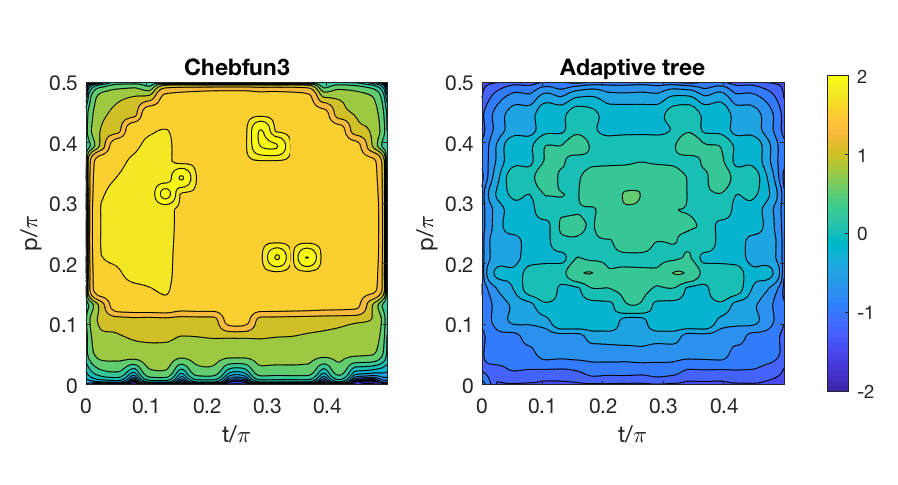
\includegraphics[width=\textwidth]{Chapter2/tan3d_comparison}
  \caption{Construction time comparison for the 3D function $\arctan(5(\sin(p)\cos(t)x+\sin(p)\sin(t)y+\cos(p)z))$, with varying angles. Colors and contours correspond to the base-10 log of execution time in seconds.}
  \label{fig:tan3D}
\end{figure}

\section{Extension to nonrectangular domains}
\label{sec:general-domain}

We now consider approximation over a nonrectangular domain $\Omega\subset \R^d$. In our construction, a leaf node $\nu$ whose domain $\Omega_\nu$ lies entirely within $\Omega$ can be treated as before. However, if $\Omega_\nu\cap \Omega \subsetneq \Omega_\nu$, we use a different approximation technique on $\nu$. The refinement criteria of Algorithm~\ref{alg:refine} are also modified for this situation.

\subsection{Algorithm modifications}


On a leaf whose domain extends outside of $\Omega$, we again use a tensor-product Chebyshev polynomial as in~(\ref{eq:full-interp}), but choose its coefficient array $C$ by satisfying a discrete least squares criterion:
\begin{equation}
  \argmin_{C} \sum_{i=1}^{P} \lp f(\vect{x}_i) -  \tilde{p}(\vect{x}_i) \rp^2,
\end{equation}
where $\Xi = \{\vect{x}_i\}_{i=1}^{P} \subset \Omega_\nu\cap \Omega$ is a point set in the ``active'' part of the leaf's domain, $\Omega_\nu\cap \Omega$. In practice we can form a matrix $A$ whose columns are evaluations of each basis function at the points in $\Xi$, leading to a standard $P\times N^d$ linear least squares problem. We choose $\Xi$ as the part of the standard $(2N)^d$-sized Chebyshev grid lying inside $\Omega$. 

This technique resembles Fourier extension or continuation techniques~\cite{adcock2014resolution,huybrechs2010fourier}, so we refer to it as a \emph{Chebyshev extension approximation}. Unlike the Fourier case, however, there is no real domain extension involved; rather one constrains the usual multivariate polynomial only over part of its usual tensor-product domain. The condition number of $A$ in the Fourier extension case has been shown to increase exponentially with the degree of the approximation \cite{adcock2014numerical}, because the collection of functions spanning the approximation space is a \emph{frame} rather than a basis. We see the same phenomenon with Chebyshev extension; essentially, constraining the polynomial over only part of the hypercube leaves it underdetermined. To cope with the numerical rank deficiency of $A$, we rely on the basic least-squares solution computed by the MATLAB backslash. We found this to be as good as or better than the pseudoinverse with a truncated SVD. 

We modify Algorithm~\ref{alg:split} so that when a domain is split, the resulting zones of the children are shrunk if possible to just contact the boundary of $\Omega$. (An exception is the shared interface between the newly created children, which is fixed.) This helps to keep a substantial proportion of a leaf's domain within $\Omega$.

We also modify how refinement decisions are made and executed in Algorithm~\ref{alg:refine}, for a subtle reason. The original algorithm is able to exploit the very different resolution requirements for a function such as, say, $xT_{60}(y)$, by testing for sufficient resolution in each dimension independently and splitting accordingly. We find experimentally that if the function is like this over $\Omega$, the extension of it to the unconstrained part of the leaf node's domain has uniform resolution requirements in all variables. Therefore, we use a simpler refinement process: if the norm of the least-squares residual (normalized by $\sqrt{P}$) is not acceptably small, we split in all dimensions successively. In effect, the approximation becomes a quadtree or octree within those nodes that do not lie entirely within $\Omega$. 


% \begin{algorithm}
% \caption{split($\Omega$,$\nu$,$j$,$t$)}
% \label{alg:LSsplit}
% \begin{algorithmic}
% \IF{$\nu$ is a leaf}
% \STATE \textsf{splitdim}($\nu$)=$j$
% \STATE Define new nodes $\nu_0$, $\nu_1$
% \STATE $[a_1,b_1],[a_2,b_2],\dots,[a_n,b_n]$ be the subintervals from \prop{zone}{$\nu$}
% \STATE Let $m:= \frac{b_j+a_j}{2}$
% \STATE Let \textsf{zone}($\nu_0$) $:= [a_1,b_1] \times \dots \times [a_{j-1},b_{j-1}] \times [a_{j},m] \times [a_{j+1},b_{j+1}] \times \dots \times [a_{d},b_{d}] $
% \STATE Let \textsf{zone}($\nu_1$) $:= [a_1,b_1] \times \dots \times [a_{j-1},b_{j-1}] \times [m,b_{j}] \times [a_{j+1},b_{j+1}] \times \dots \times [a_{d},b_{d}] $
% \FOR{$k=0,1$}
% \STATE Define \textsf{domain}($\nu_k$) from \textsf{zone}($\nu_k$) with parameter $t$ as in~(\ref{eq:zone_extend})
% \IF{$\text{\textsf{domain}($\nu_k$)} \cap \Omega = \emptyset$}
% \STATE $\nu_k$ = NULL
% \ELSIF{$\text{\textsf{domain}($\nu_k$)} \subseteq \Omega$}
% \STATE define $\nu_k$ as node on a hypercube.
% \ELSE
% \STATE For dimensions $p=1,2,\dots,j-1,j+1,\dots,d$ change subintervals $[a_p,b_p]$ of \textsf{domain}($\nu_k$) and \textsf{zone}($\nu_k$) to fit $\Omega$.
% \STATE For dimension $p=j$, change subinterval $[a_p,b_p]$ of \textsf{domain}($\nu_k$) by choosing largest $a_p$ such that $\Omega \subset \text{\textsf{domain}($\nu_k$)}$ if $k=0$, and vice versa if $k=1$. Change endpoints of \textsf{zone}($\nu_k$) to match changed endpoints of \textsf{domain}($\nu_k$).
% \ENDIF
% \STATE Define \textsf{grid}($\nu_k$) as Chebyshev tensor-product grid of size $\nmax^d$ in \textsf{domain}($\nu_k$)
% \STATE Let \textsf{isdone}($\nu_k$):= \textsf{isdone}($\nu$)
% \ENDFOR
% \ELSE
% \STATE split(\child{0}($\nu$),$k$,$t$)
% \STATE split(\child{1}($\nu$),$k$,$t$)
% \ENDIF
% \end{algorithmic}
% \end{algorithm}

\subsection{Numerical experiments}

We chose the test functions 
\begin{equation}
  \label{eq:testfun-gen}
  \begin{aligned}
    g_1& =\exp(x+y), & g_2&=\dfrac{1}{((x-1.1)^2)+(y-1.1)^2)^2}, \\
    g_3 &=\cos(24x-32y)\sin(21x-28y), & g_4&=\arctan(3(x^2+y)).
  \end{aligned}
\end{equation}
We approximated each function on each of three domains: the unit disk, the diamond $|x|+|y|\le 1$, and the double astroid seen in Figure~\ref{star_plot}. The initial box (root of the approximation tree) was chosen to tightly enclose the given domain. For each test we set $N=17$ and the target tolerance to $10^{-10}$. We timed both the adaptive construction and the evaluation on a $200\times 200$ grid, and recorded the max error as in the previous section. In each case, we choose initial box to fit the domain as tightly as possible. These results can be seen in Table~\ref{table_general}. The resulting approximation of $g_4$ on the double astroid is shown in Figure~\ref{star_plot}, along with the adaptively found subdomains. 

When the function is smooth or contains localized features, we find that the method is both efficient and highly accurate; in the smoothest case of $g_1$, a global multivariate least-squares polynomial is sufficient. Only for $g_3$, which requires uniformly fine resolution throughout the domains, is there a construction time longer than a few seconds. The Fourier extension methods described in~\cite{matthysen2017function} are implemented in Julia, making a direct quantitative comparisons difficult, but based on the orders of magnitude of the results reported there, we feel confident that our results for these examples are superior. 


% \begin{figure}
% \centering

% \subfloat[Diamond domain]{
% 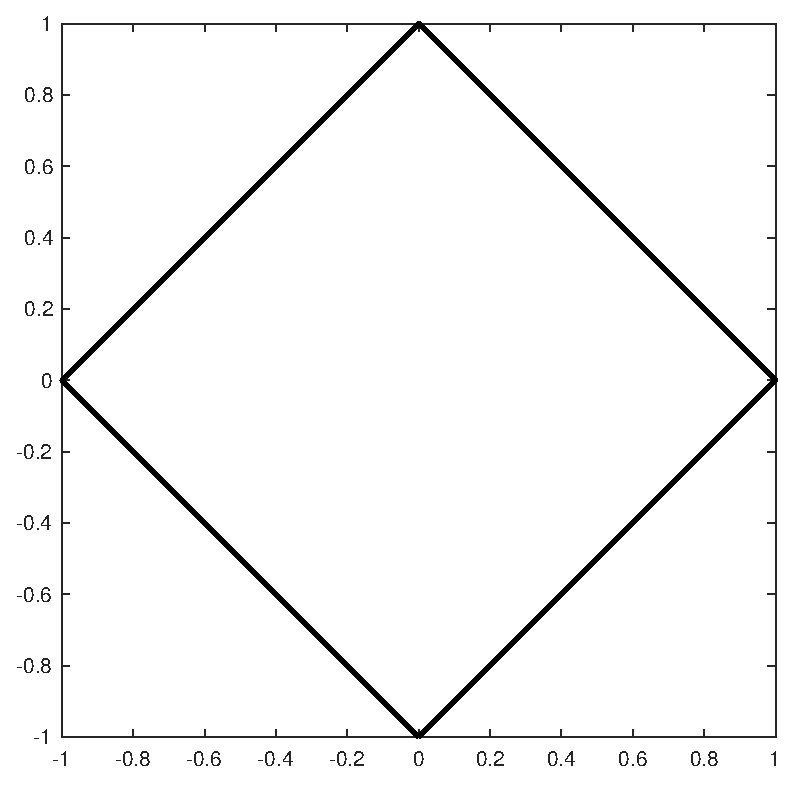
\includegraphics[scale = 0.3]{diamond.eps}
%    \label{domain_b}
%  }
%  \subfloat[Double astroid domain]{
% 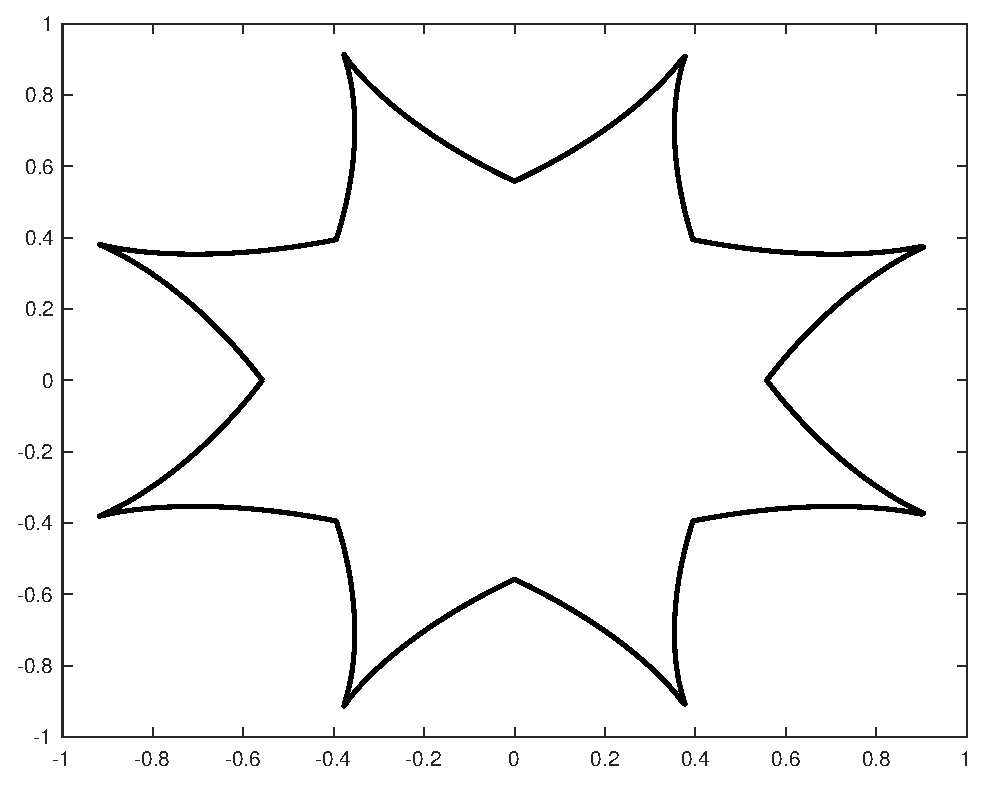
\includegraphics[scale = 0.3]{star.eps}
%    \label{domain_c}
%  }
%  \caption{Plots of the domains we tested on 2D. The double astroid domain is the union of two rotated astroid curves.}
% \label{domains}
% \end{figure}

\begin{figure}
\centering
\subfloat[Plot of $\arctan(3(y^2+x))$.]{
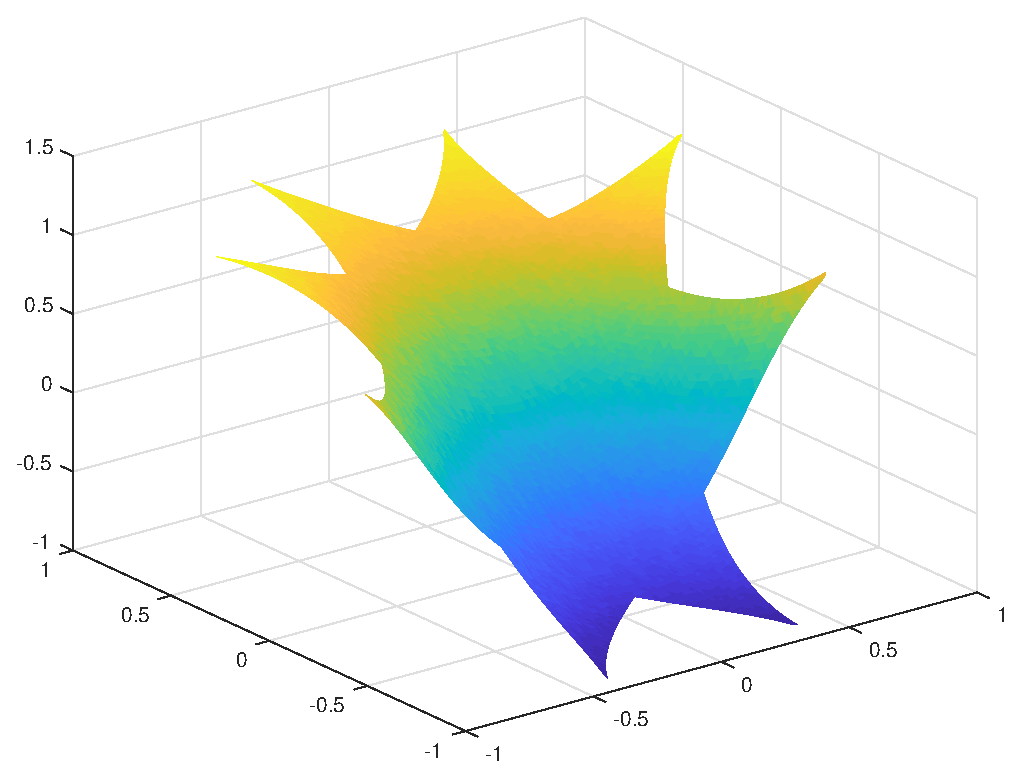
\includegraphics[scale = 0.34]{Chapter2/starPlot.eps}
   \label{star_plota}
 }
\subfloat[Plot of subdomains.]{
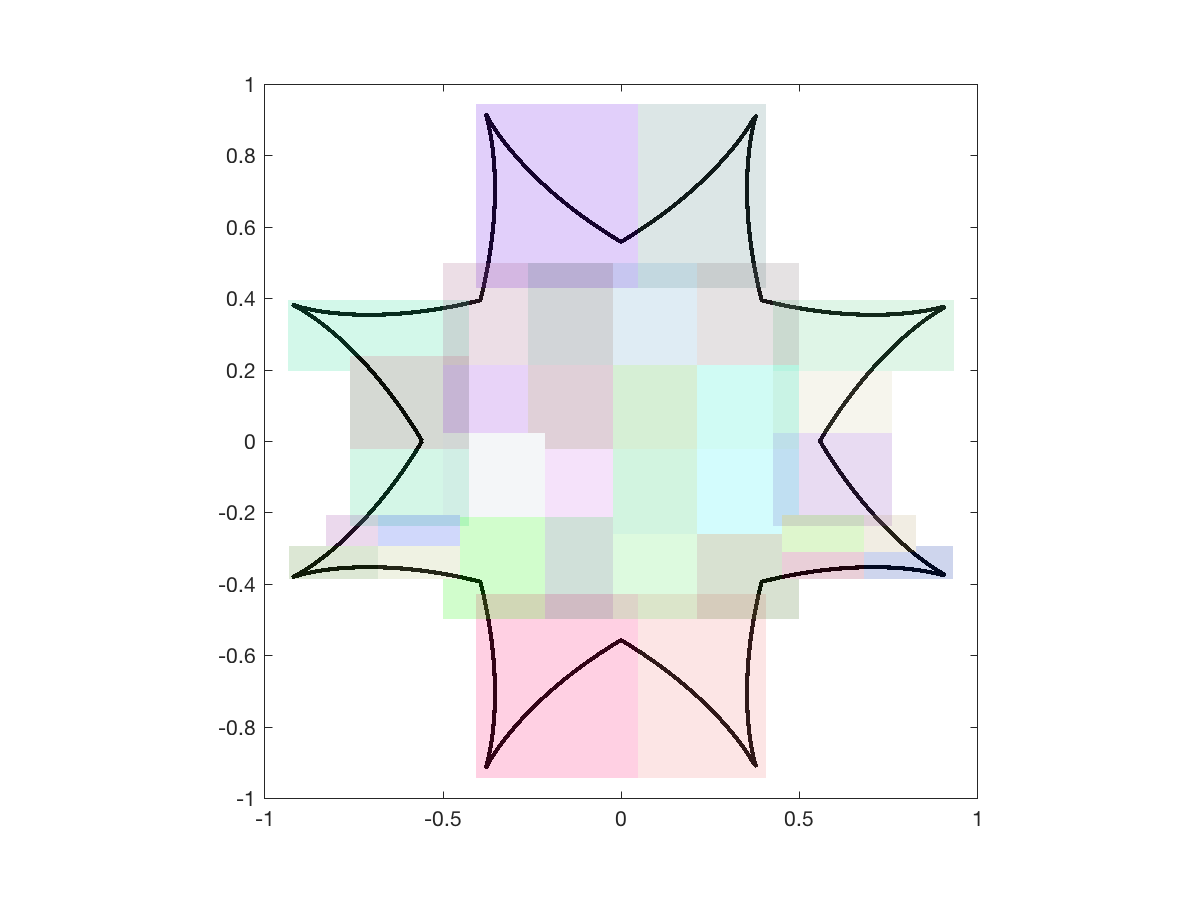
\includegraphics[scale = 0.34]{Chapter2/starPlotDoms.eps}
   \label{star_plotb}
 }
\caption{Plot of $\arctan(3(y^2+x))$ and the subdomains formed from the partition of unity method. The error in this approximation was found to be about $10^{-11}$.}
\label{star_plot}
\end{figure}


\begin{table}
\begin{tabular}{c|c|c|c|c|c}
function & domain & error & construct time & interp time & points \\ [5pt] \hline
\multirow{3}{*}{ $g_1$ } & disk & 5.44E-15 & 1.369 & 0.012 & 289 \\
& diamond & 2.06E-11 & 0.040 & 0.002 & 289 \\
& astroid & 2.01E-08 & 0.071 & 0.001 & 289 \\ \hline
\multirow{3}{*}{ $g_2$ } & disk & 2.40E-10 & 2.558 & 0.117 & 3757 \\
& diamond & 2.40E-11 & 0.406 & 0.012 & 2023 \\
& astroid & 2.14E-10 & 1.511 & 0.023 & 4624 \\ \hline
\multirow{3}{*}{ $g_3$ } & disk & 4.44E-11 & 11.305 & 1.500 & 245650 \\
& diamond & 2.35E-11 & 10.894 & 0.854 & 178020 \\
& astroid & 1.67E-10 & 28.072 & 0.836 & 153780 \\ \hline
\multirow{3}{*}{ $g_4$ } & disk & 7.49E-11 & 1.866 & 0.059 & 12138 \\
& diamond & 1.45E-11 & 1.536 & 0.053 & 9826 \\
& astroid & 1.09E-11 & 3.221 & 0.049 & 9826 \\
\end{tabular}
  \caption{Observed error and wall-clock times for the adaptive tree method to approximate the functions given in~(\ref{eq:testfun-gen}) on three different 2D domains. Also shown is the total number of sampled function values stored over all the leaves of each final tree.}
  \label{table_general}
\end{table}


\section{Discussion}
\label{sec:conclusion}

For functions over hyperrectangles of uncorrelated variables or that otherwise are well-aligned with coordinate axes, low-rank and sparse-grid approximations can be expected to be highly performant. We have demonstrated an alternative adaptive approach that, in two or three dimensions, typically performs very well on such functions but is far less dependent on that property. Our method sacrifices the use of a single global representation that could achieve true spectral convergence, but in practice we are able to use a partition of unity to construct a smooth, global approximation of very high accuracy in a wide range of examples. 

The adaptive domain decomposition offers some other potential advantages we have not yet exploited, but are studying. It offers a built-in parallelism for function construction and evaluation. It allows efficient updating of function values locally, rather than globally, over the domain. Finally, it has a built-in preconditioning strategy, based on additive Schwarz methods, for the solution of partial differential equations.

By replacing tensor-product interpolation on the leaves with a simple least-squares approximation using the same multivariate polynomials, we have been able to demonstrate at least reasonable performance in approximation over nonrectangular domains. Further investigation is required to better understand the least-squares approximation process, optimize adaptive strategies, and find efficient algorithms for merging trees and operations such as integration.    % This file (chap2.tex) contains the text

                   % for Chapter 2.

%%
% This is the References file (ref.tex)
%
\renewcommand{\bibname}{References}
\begin{thereferences}
Lastname, Firstname  ``Title.''  \textit{Journal}, Year.

Lastname, Firstname, and Firstname Lastname.  \textit{Title of Book}.  Publisher, Year.
\end{thereferences}
      % This file (ref.tex) contains the text
                   % for the references.
                   
%%
% This is the Bibliography file (bib.tex)
%
% For 100-999 change 99 to 999; for 1000-9999 change 99 to 9999 
\begin{thebibliography}{99}
\bibitem{1}Lastname, Firstname  ``Title.''  \textit{Journal}, Year.

\bibitem{2}Lastname, Firstname, and Firstname Lastname.  \textit{Title of Book}.  Publisher, Year.
\end{thebibliography}
      % This file (bib.tex) contains the text
                   % for a bibliography.
                                      
%
% This is the Bibliography file (bibtex.tex)
% This generally works for BibTeX

% Use sample.bib for BibTeX database
\bibliography{Chapter1/PU_BIB,Chapter2/PU_BIB,Chapter3/schwarz}
% BibTeX style (plain, alpha, unsrt)
\bibliographystyle{plain}
	 % This file (bibtex.tex) contains the text
                   % for a bibliography if using BibTeX with
                   % sample.bib
                                      
%%
% This is one Appendix file (app.tex)
%
\oneappendix{Title for Appendix}

This is the information for one appendix. This is to be used if there is only one appendix.      % This file (app.tex) contains the text
                   % for one Appendix. 
                   
%
% This is the Appendix A file (appA.tex)
%
\appendix{Title of Appendix}

This is the information for the first appendix, Appendix A. Copy the base file, appA.tex, for each additional appendix needed such as appB.tex, appC.tex, etc. Modify the main base file to include each additional appendix file.

If there is only one appendix, then modify the main file to only use app.tex instead of appA.tex.     % This file (appA.tex) contains the text
                   % for Appendix A. 
                   
%
% This is the Appendix A file (appA.tex)
%
\appendix{Flux functions and initial condition}
\label{sec:flux}

We define the influx and outflux functions $Q_{lg}$, $Q_{p}$ to be bump functions in space and time. With
\begin{equation}
\step(x,a,b) = 1/2 (1 + \tanh[(4 (a + b - 2 x))/(a - b)]),
\end{equation}
we define a indicator like bump function
\begin{equation}
w(x,a,b,l) = \step(x,a,a+l)-\step(x,b-l,b)
\label{indicator_fun}
\end{equation}
that has support on $[a,b]$ but continuously drops from 1 to 0 in intervals of length $l$. Here $w$ effectively is a smooth approximation of an indicator function. 

 With this bump function and a blink cycle with period $L$, we define
\begin{eqnarray}
\hat{Q_{lg}}(\hat{x},t) &= w(t,0.02,0.5 L,0.1) \exp(((\hat{x}-0.5)/0.25)^2), \label{bumb_funs}  \\
\hat{Q_{p}}(\hat{y},t) &= w(t,0.05,0.5 L,0.1) w(\hat{y},-0.9,0.25,0.9). 
\end{eqnarray}
With target supply and drain volumes $V_s, V_d$ over a blink cycle, we normalize the flux functions (\ref{un_flux}) to define $Q_p,Q_{\lg}$:
\begin{eqnarray}
Q_{lg}(\hat{x},t) &= \frac{V_s}{\int_{0}^{p} \int_{-1}^1 \hat{Q_{lg}} d\hat{x} dt} \hat{Q_{lg}}(\hat{x},t), \label{un_flux1} \\
Q_{p}(\hat{y},t) &= \frac{V_d}{\int_{0}^{p} \int_{-1}^1 \hat{Q_{p}} d\hat{y} dt} \hat{Q_{p}}(\hat{y},t).
\label{un_flux}
\end{eqnarray}
The influx function $Q_{lg}$ is defined so there is an influx of fluid from the top of the lid, concentrated in the center; this is simulated with the use of an exponential bump function, as seen in (\ref{un_flux1}). The influx occurs for $t \in [0.02,0.5 L]$. The ouflux function $Q_p$ defines a drainage through the puncta; $Q_p$ is defined on the left corner of the eye-shaped domain. The outflux occurs evenly throughout the corner, as seen with the use of the indicator like function (\ref{indicator_fun})  in (\ref{un_flux}). The outflux occurs within $t \in [0.05,0.5 L]$, starting after an initial influx of fluid. A plot of the flux functions at different times throughout the blink cycle can be seen in Figure~\ref{flux_plots}.

\begin{figure}
	\centering
	\subfloat[]{
		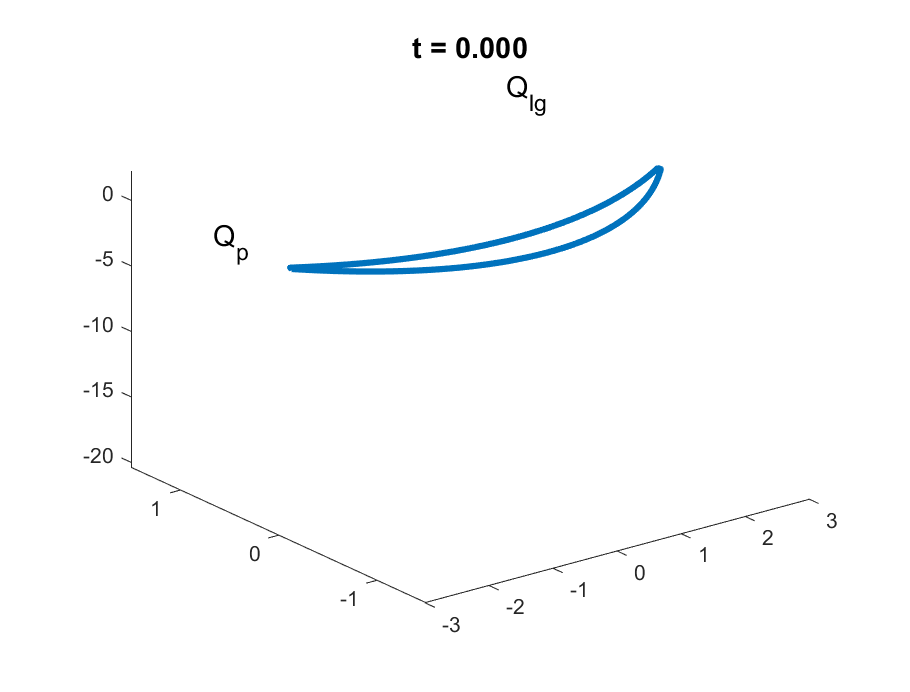
\includegraphics[scale = 0.4]{Chapter4/fluxfuns1}
		\label{flux_plot1}
	}
	\subfloat[]{
		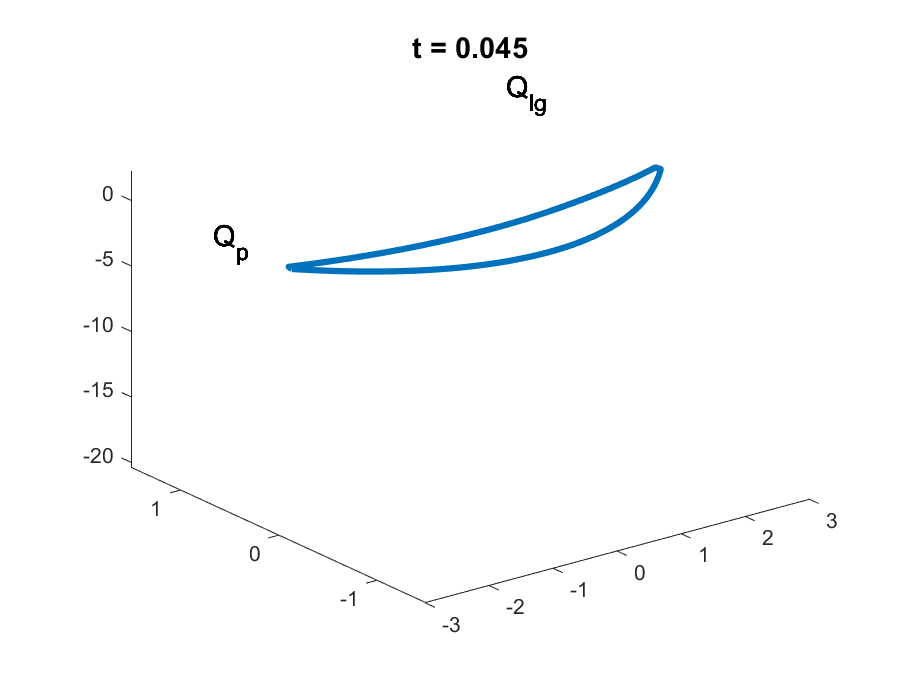
\includegraphics[scale = 0.4]{Chapter4/fluxfuns2}
		\label{flux_plot2}
	} 
	
	\subfloat[]{
		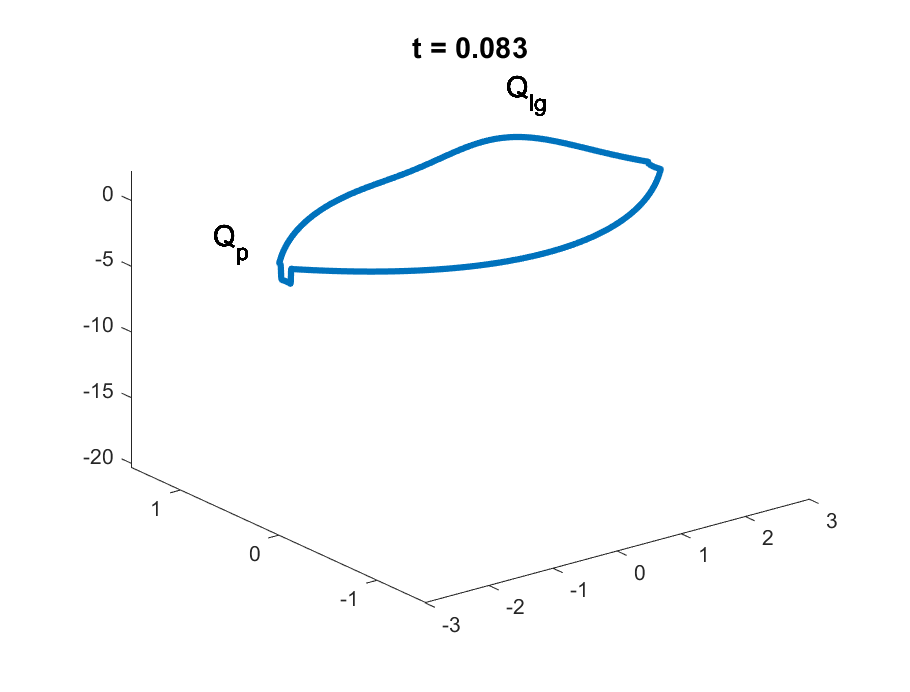
\includegraphics[scale = 0.4]{Chapter4/fluxfuns3}
		\label{flux_plot3}
	}
	\subfloat[]{
		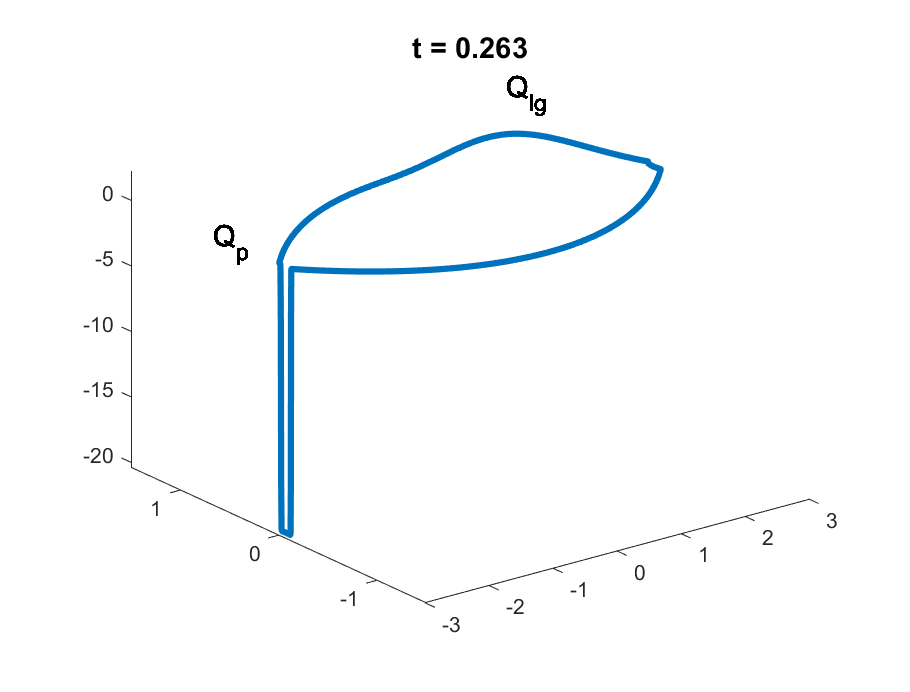
\includegraphics[scale = 0.4]{Chapter4/fluxfuns4}
		\label{flux_plot4}
	} 
	
	\subfloat[]{
		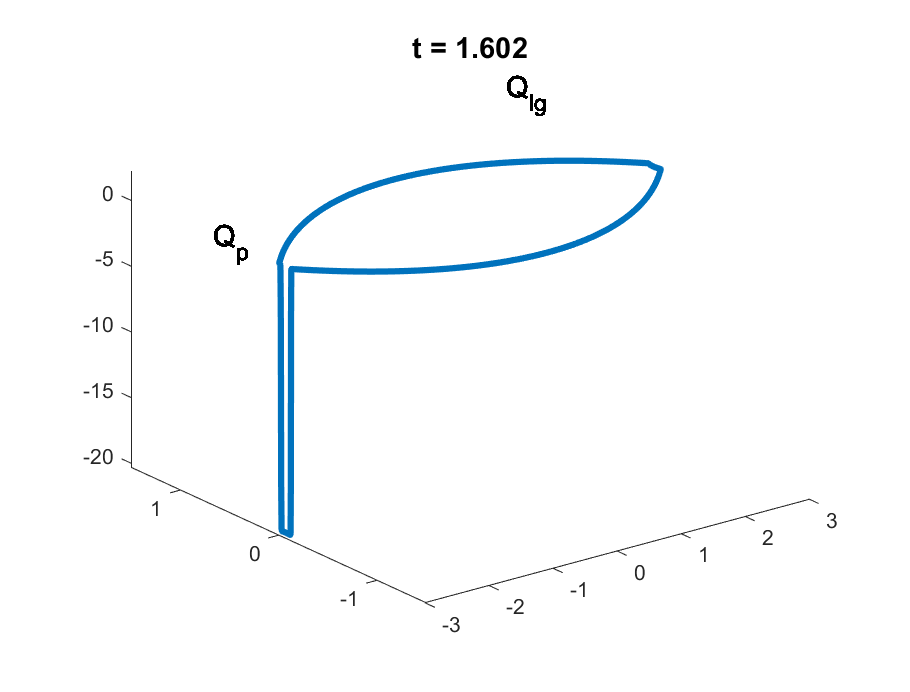
\includegraphics[scale = 0.4]{Chapter4/fluxfuns5}
		\label{flux_plot5}
	}
	\subfloat[]{
		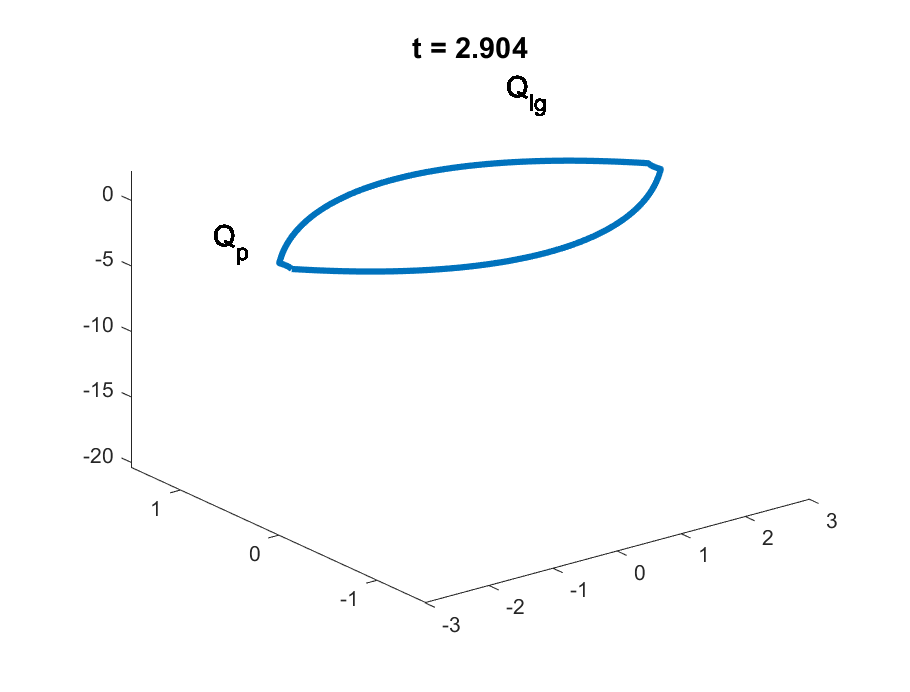
\includegraphics[scale = 0.4]{Chapter4/fluxfuns6}
		\label{flux_plot6}
	}
	
	\caption{Plot of the flux functions (\ref{un_flux1},\ref{un_flux}) at different times throughout the blink cycle. At the start of the blink cycle both fluxes are 0. Then at $t=0.02$, an influx of fluid starts, followed by an outflux at $t=0.05$. From $t=0.05$ to $t=0.5 L$, there is both an influx and outflux of fluid. After $t=0.5 L$, both the influx and outflux of fluid dissipates.}
	\label{flux_plots}
\end{figure}

We define the initial condition $h_I(\hat{x},\hat{y})$ implicitly by first solving
\begin{align}
\begin{aligned}
\nabla^2 \hat{h_I} &= 10 (\hat{x}^4 +\hat{y}^4) \quad (\hat{x},\hat{y}) \in \mathcal{C} \\
\hat{h_I} &= 1 \mbox{ on } \partial \mathcal{C},
\end{aligned} 
\end{align}
and finding coefficients $c_0,c_1$ so that the initial condition
\begin{equation}
h_I(\hat{x},\hat{y}) = c_1 \hat{h_I}(\hat{x},\hat{y})+c_0
\end{equation}
matches $h_0$ on the boundary and numerically has a prescribed volume $V_{\mbox{init}}$. This initial condition produces a solution with boundary layers, as seen in Figures~\ref{tears_02_1},\ref{broken_tears_0}.     % This file (appB.tex) contains the text
                   % for Appendix B.   
       
\end{document}